\section{Evaluation}

Having explained the details of the environment and the algorithms used, this section will go into detail about the details of the configuration of the experiments and the results of the experiments. The details of the training configuration for each algorithm and the reason for these decisions will be discussed. For each algorithm compared, the best perfoming agent will be determined and chosen to be used as the agent to be compared to the other best performing agents. When deciding the best performing agent, multiple factors will be considered such as the total reward, loss, amount of exploration and amount of battling. The results of the experiments will be discussed, compared to each other and evaluated to determine how well they were able to balance out both battling and navigation.

\subsection{Training Configuration}

The training configuration for each algorithm was set to be the same for each algorithm. Each agent was trained for a total of 40 million steps and a gamma rate of 0.998 within the environment with a batch size of 64. Each algorithm used the default hyperparameters implemented within the stablebaselines3 library and each agent was trained with the exact same representation of the environment with no changes to the reward scaling and reward functions. 

\subsubsection{Hyperparameter Tuning}

It was mentioned previously that each algorithm would be hyperparameter tuned so that they were compared fairly. However, the hyperparameters were not tuned for each algorithm because of the amount of time it would take to tune each hyperparameter for each algorithm. It would take 5-7 hours to train a single agent, which would mean that it would take countless more for each hyperparameter for each algorithm to be tuned. Therefore, the default hyperparameters implemented by stablebaselines3 were used for each algorithm to ensure that the agents were compared fairly \cite{stablebaselines3}.

\subsection{DQN}

\begin{center}
\begin{tabular}{ |c|c| } 
 \hline
 Hyperparameter & Value \\ 
 \hline
 Total Timesteps & 40,00,500 \\
 Number of Episodes &  2,667 \\
 Episode Length & 1,500 \\ 
 Parallel Instances & 10 \\
 Policy Model & MultiInputPolicy \\
 Gamma & 0.99 \\  
 Batch Size & 64 \\
 \hline
\end{tabular}
\end{center}

The training script used to train all 4 agents can be found within the research paper's GitHub repository under ``run\_baseline\_DQN.py''. A total of 10 parallel instances of the environment was trained at the same time to train for 2,667 episodes total, where each episode is 1,500 steps long. This totals up to 40,00,500 steps in total. The performance of the 4 agents can be seen on figure \ref{fig:agent_eval_all_dqn}. 


\subsubsection*{Total Reward}

\begin{figure}[H]
    \centering
    \subfigure[DQN-1]{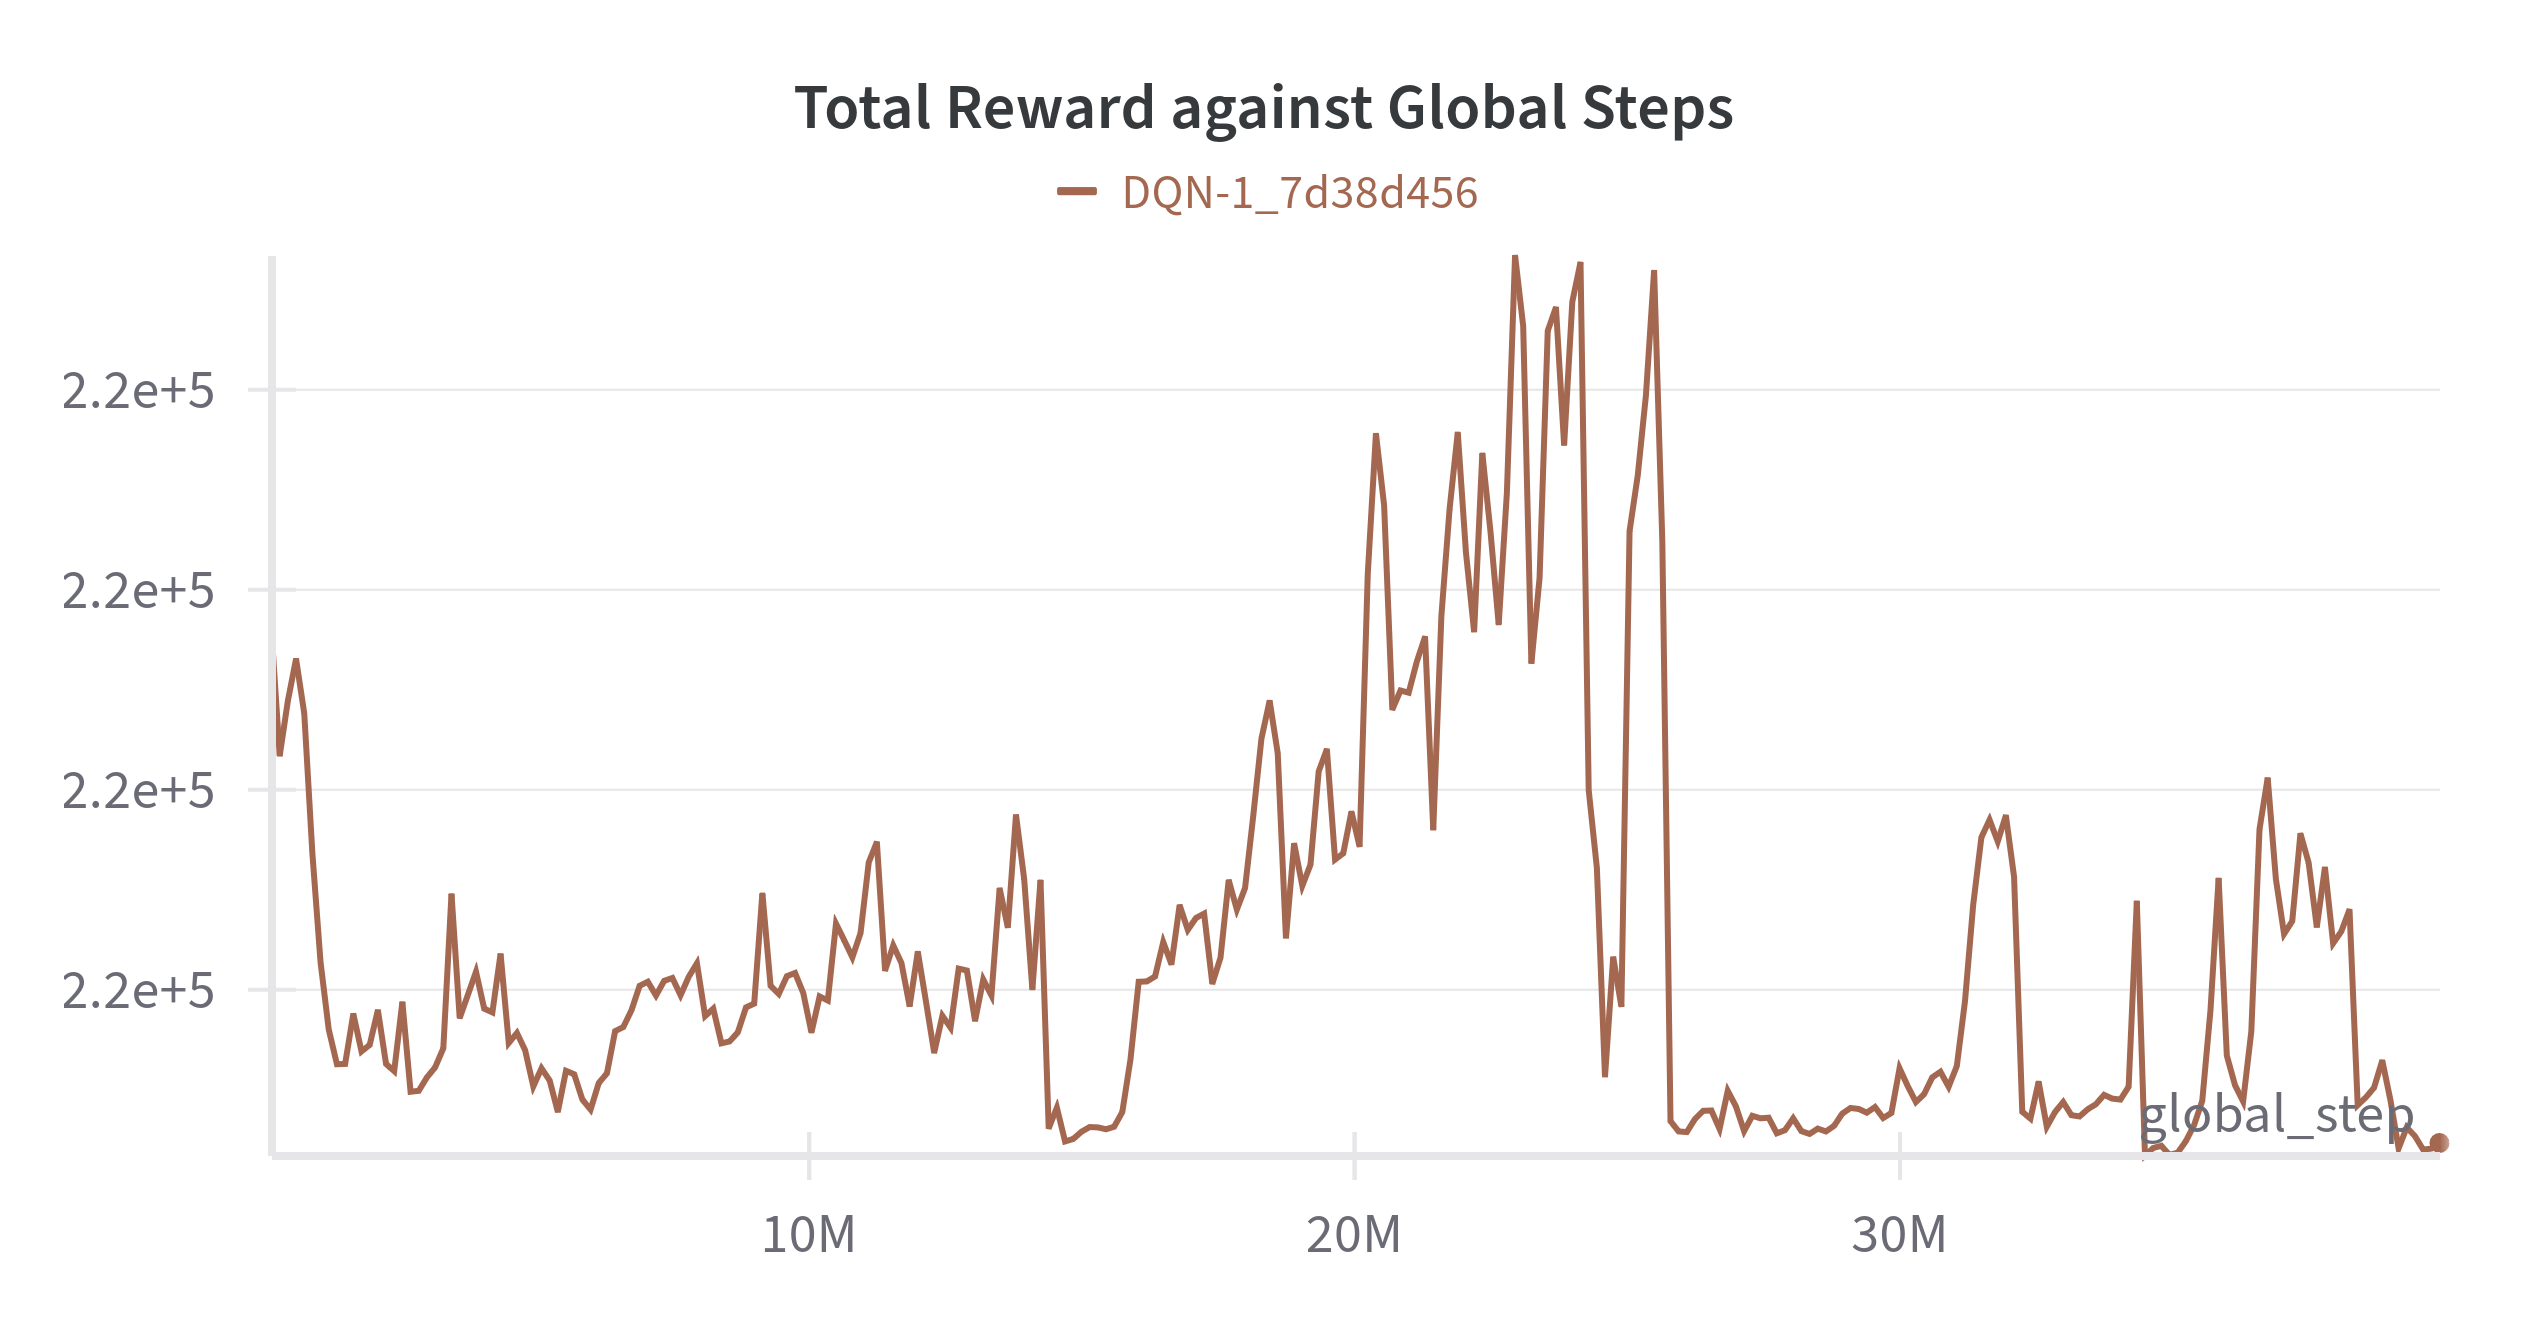
\includegraphics[width=0.49\textwidth]{figures/DQN/DQN1_Total_Reward.png}} 
    \subfigure[DQN-2]{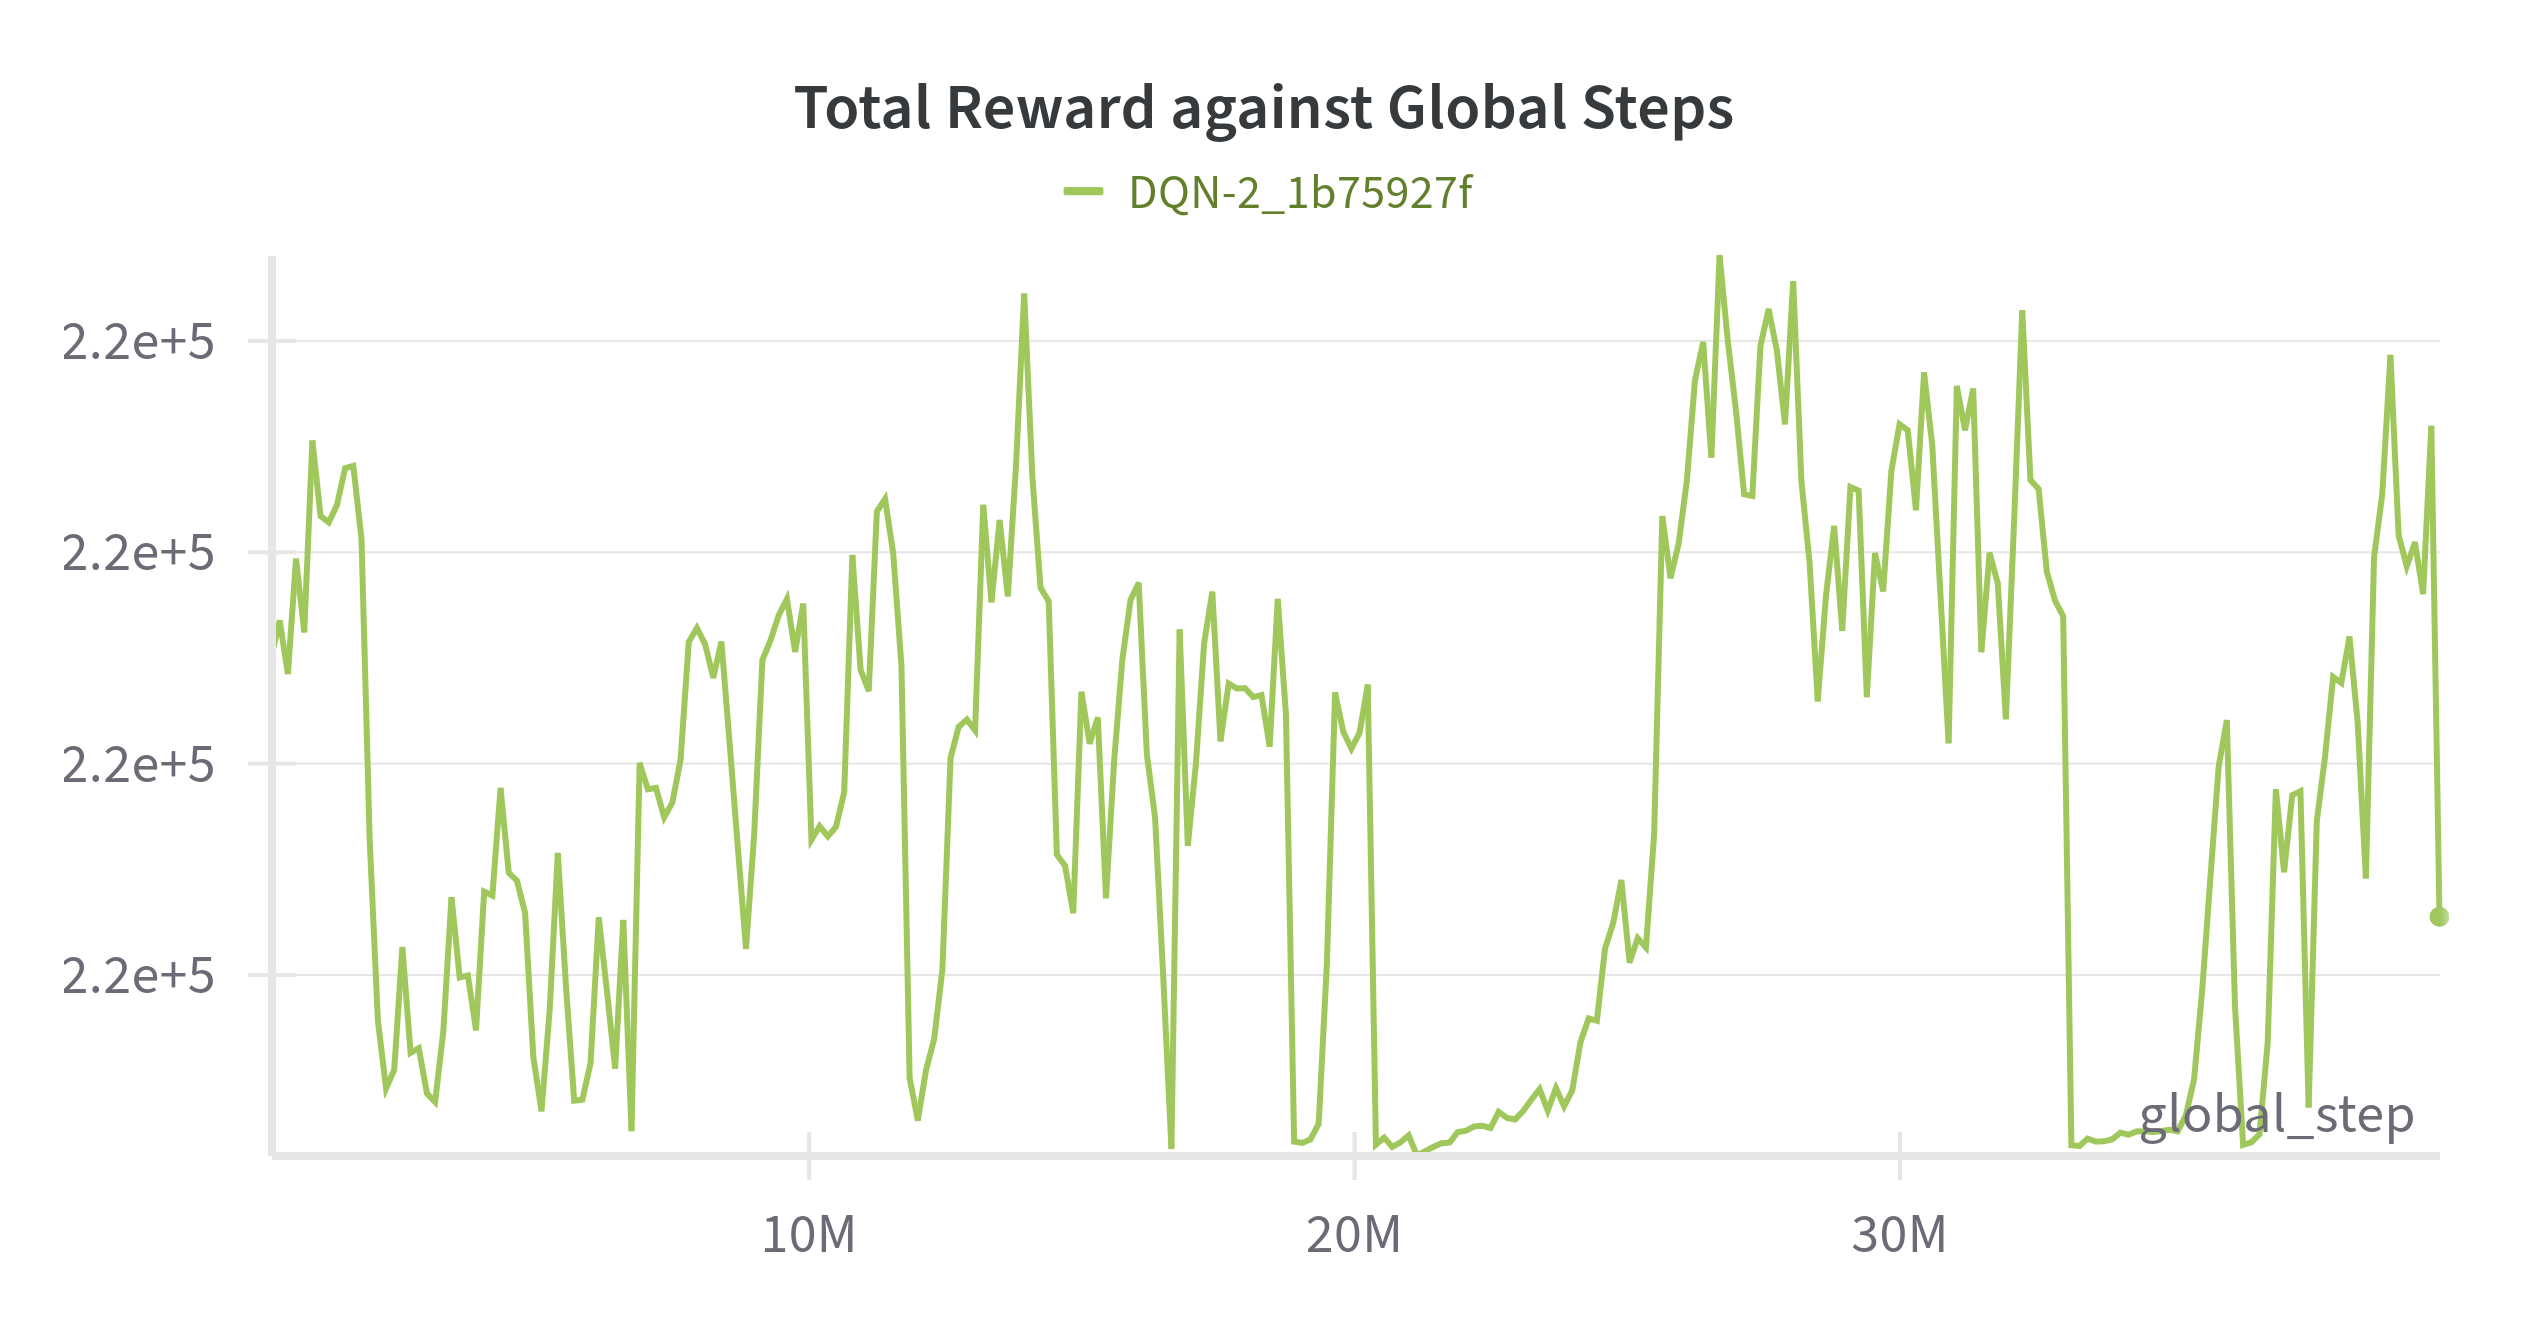
\includegraphics[width=0.49\textwidth]{figures/DQN/DQN2_Total_Reward.png}} 
    \subfigure[DQN-3]{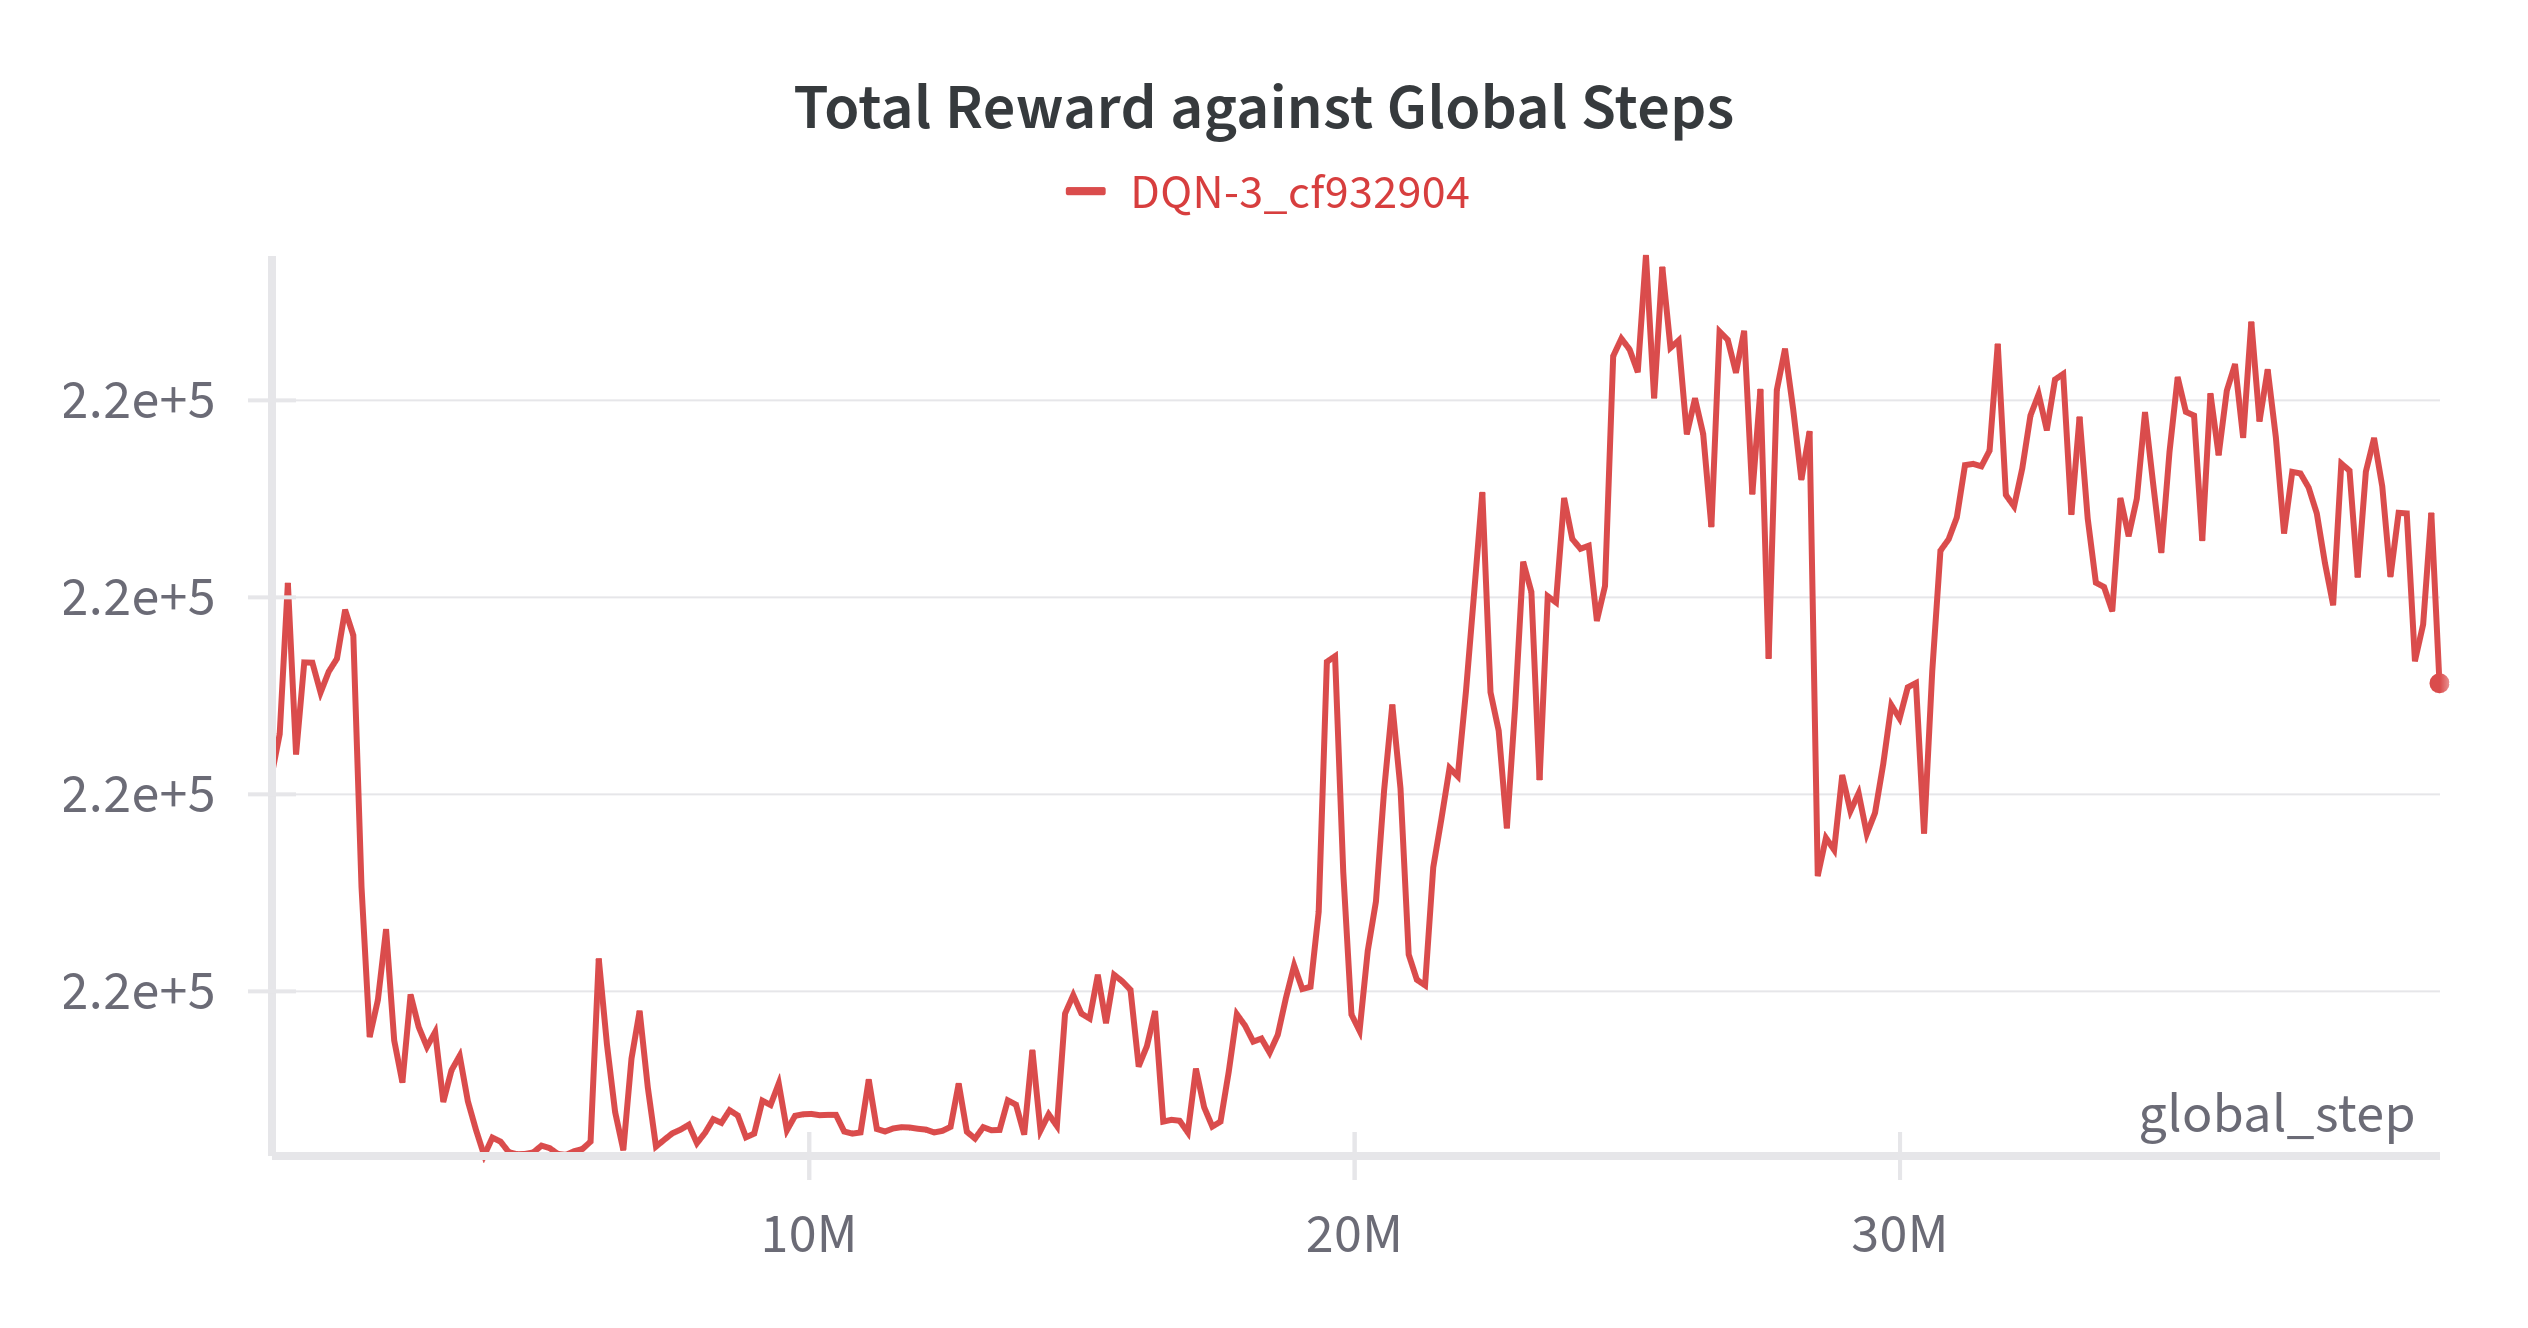
\includegraphics[width=0.49\textwidth]{figures/DQN/DQN3_Total_Reward.png}}
    \subfigure[DQN-4]{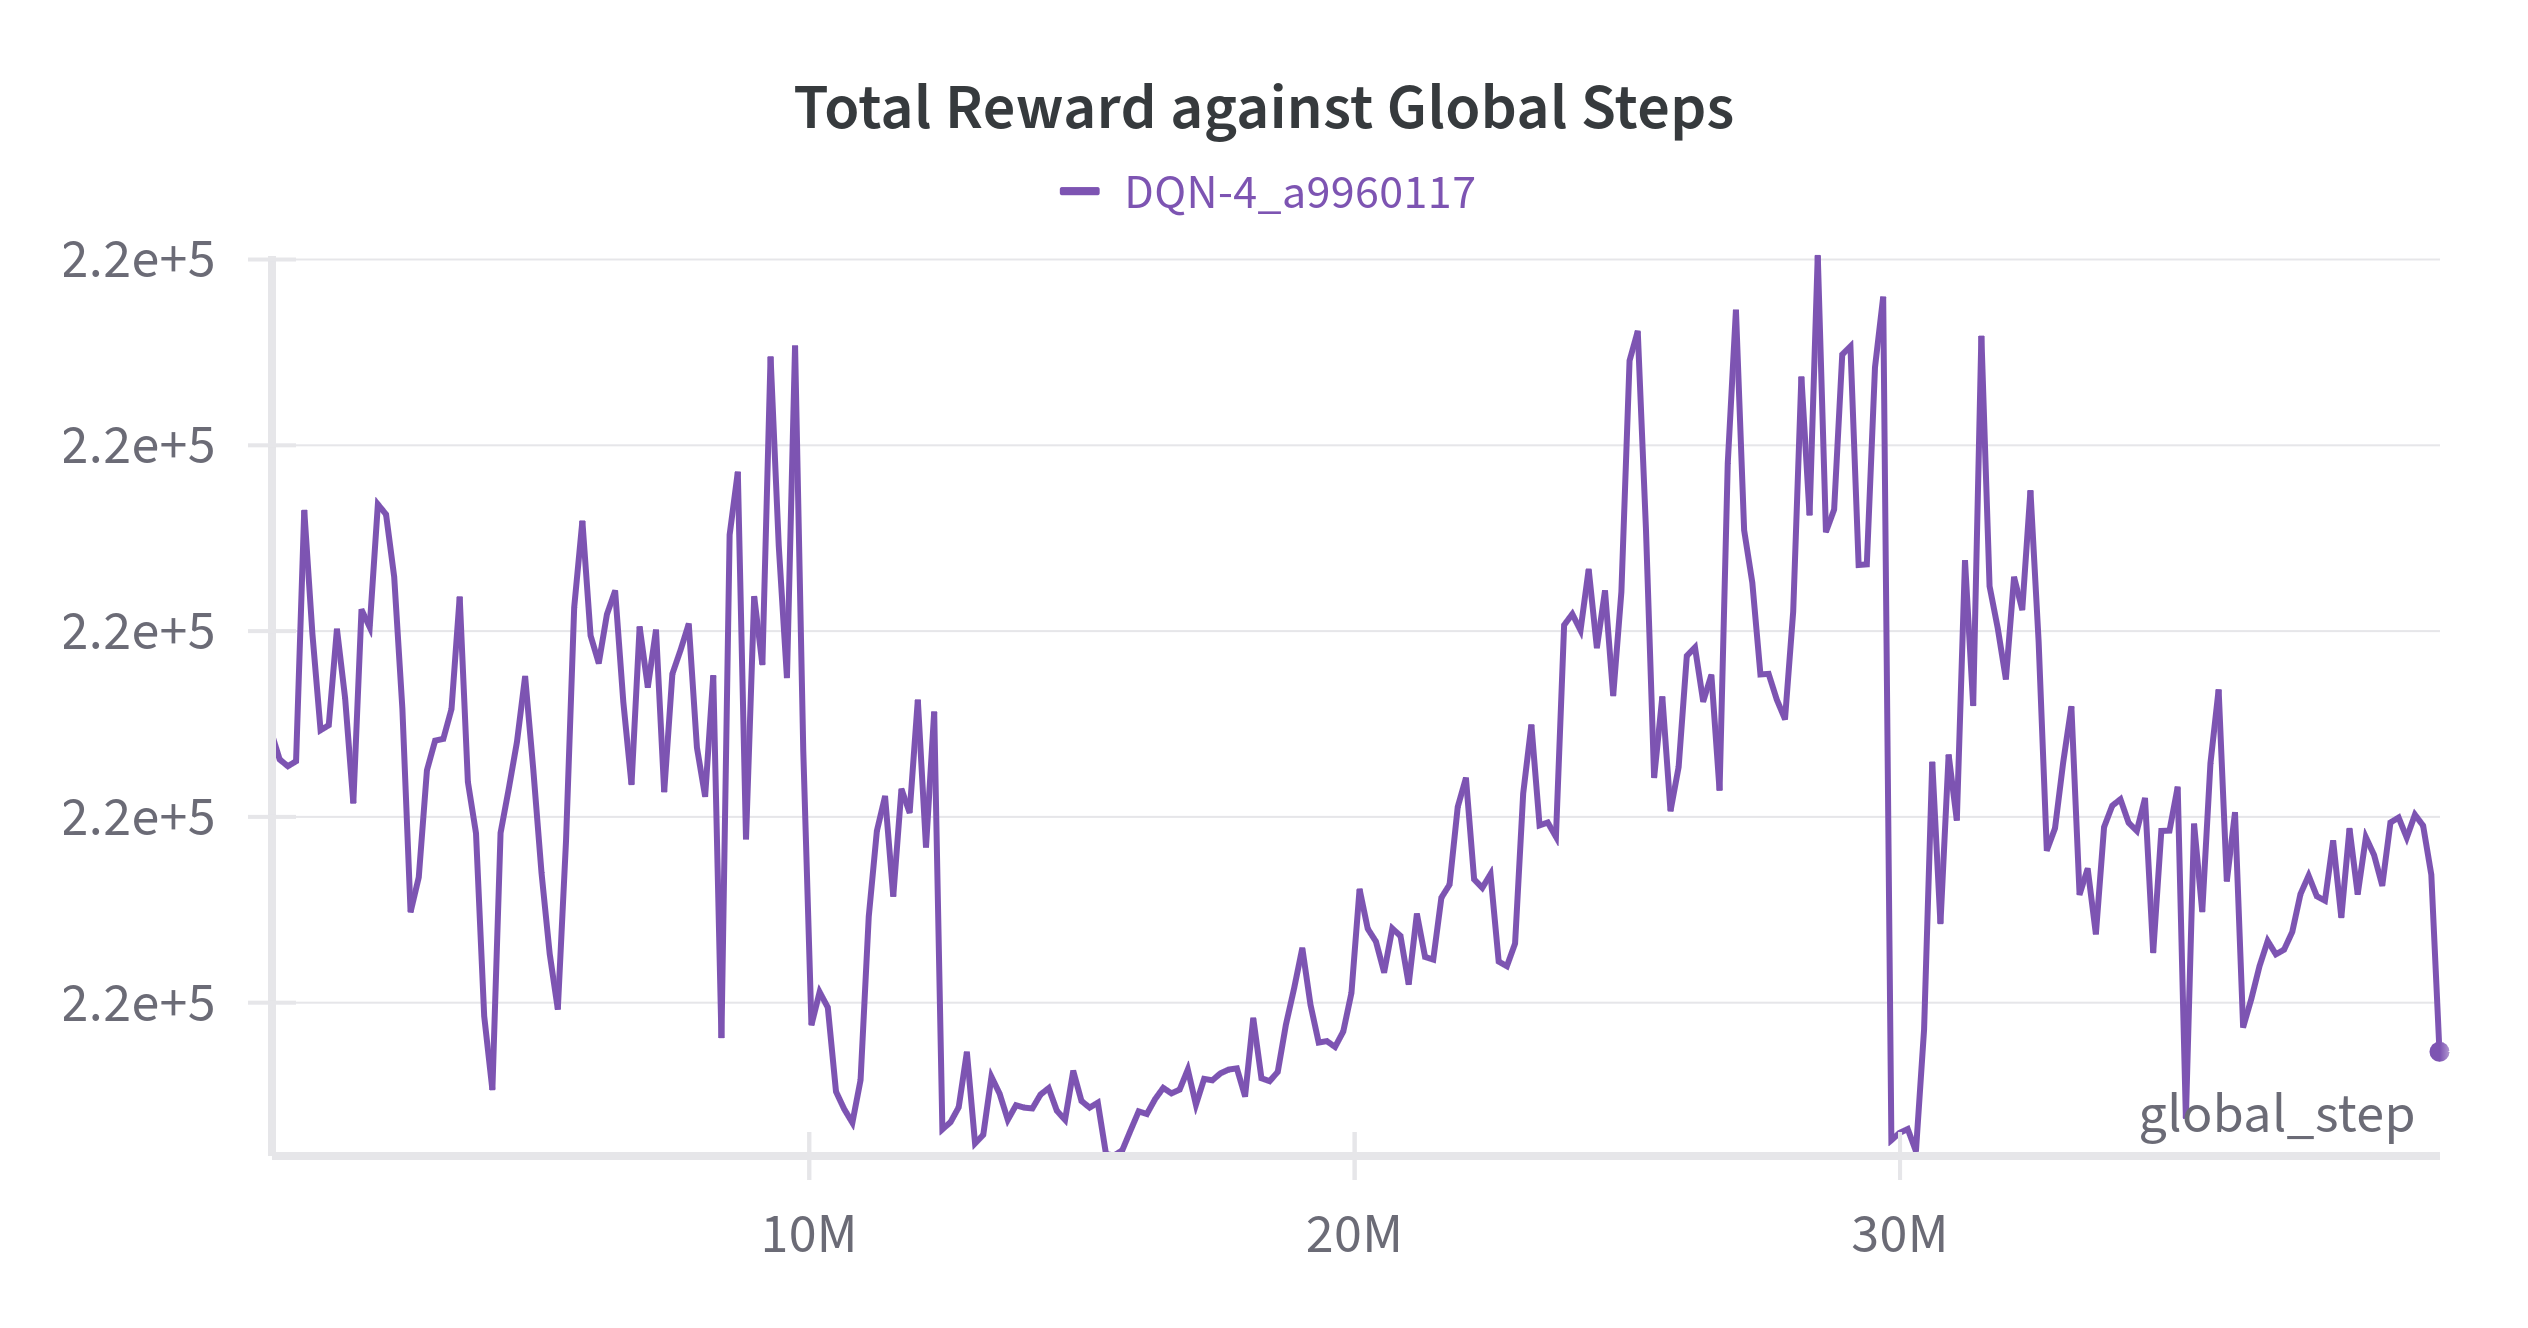
\includegraphics[width=0.49\textwidth]{figures/DQN/DQN4_Total_Reward.png}}
    \caption{Total Reward of all DQN Agents}
    \label{fig:DQN_total_reward}
\end{figure}

Figure \ref{fig:DQN_total_reward} shows the performance of all 4 DQN agents of total reward against global steps. The figure shows all 4 performing agents did not show signs of reaching the optimal policy as the total reward show a dramatic difference from the start of training to the end of training. The agents were not able to reach a consistent amount of reward throughout training, which suggests that the agents were still exploring the environment and were not able to exploit the environment using its already known information. However, given that the agents were trained for 40 million timesteps, it is possible that further training would not have resulted in a better performance.

Figure \ref{fig:DQN_total_reward} (a) shows the performance of DQN-1, which shows that the agent did not show signs of reaching the optimal policy as the performance of the agent peaked at around 150 episodes followed by a sharp fall in performance. This suggests that the agent was still exploring the environment and was not ready to start exploiting the environment using its already known information, as the sharp fall in performance was below the starting performance of the agent.

Figure \ref{fig:DQN_total_reward} (b) shows the performance of DQN-2, which shows that the agent did show signs of significant amount of exploration, as there was a range of episodes where the agent had high and low performance. This suggests that the agent was still exploring the environment. However, the agent did have a consistently high amount of performance between episodes 170 and 210.

Figure \ref{fig:DQN_total_reward} (c) shows the performance of DQN-3, which shows that the agent did show signs of exploration, as the training of the agent started with a low amount of performance and gradually increased in performance between episode 10 and 150. This suggests that the agent was able to slowly learn the environment that was trained on and shows signs of gradual learning. Moreover, the agent was able to reach a peak performance at around episode 150 and is the best performing agent out of the DQN agents so far due to its consistently high performance. 

Figure \ref{fig:DQN_total_reward} (d) shows the performance of DQN-4, which shows that the agent shows weak signs of an understanding of the environment due to its low performance throughout the training. The agent did not show any signs of consistently high performance as drops in performance always followed high peaks. This highly suggests that the agent was still exploring the environment and never reached a point where it was able to exploit the environment using its already known information.

\subsubsection*{Loss}

\begin{figure}[H]
    \centering
    \subfigure[DQN-1]{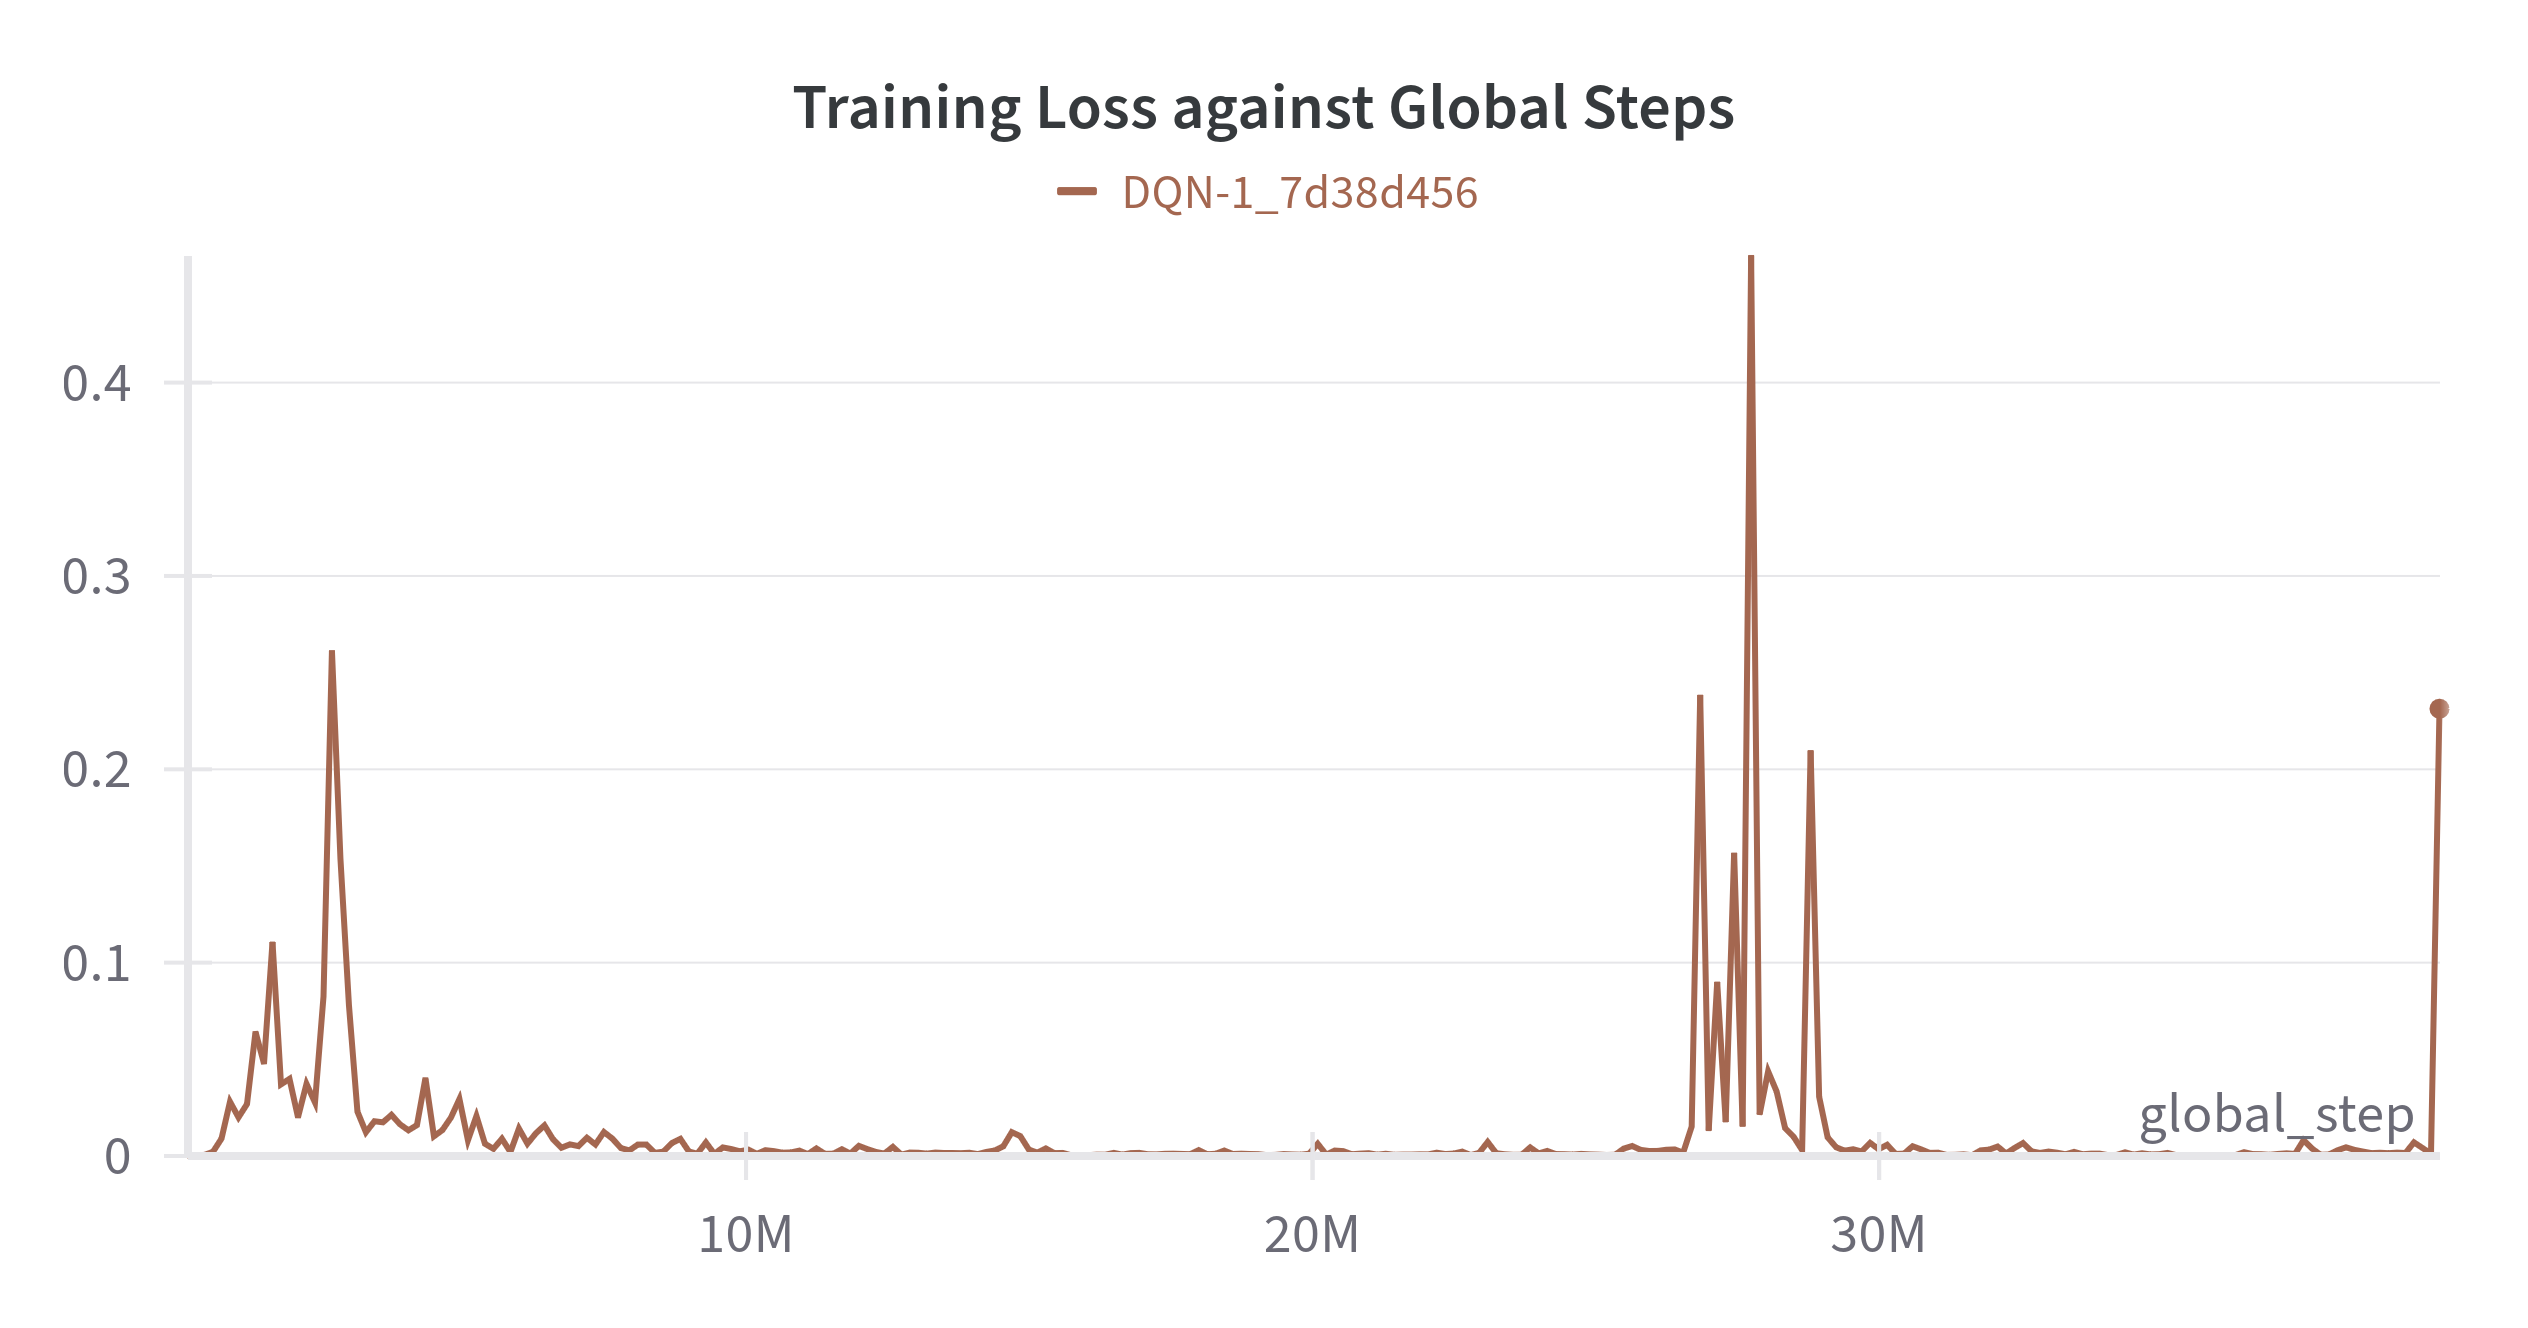
\includegraphics[width=0.49\textwidth]{figures/DQN/DQN1_Training_Loss.png}} 
    \subfigure[DQN-2]{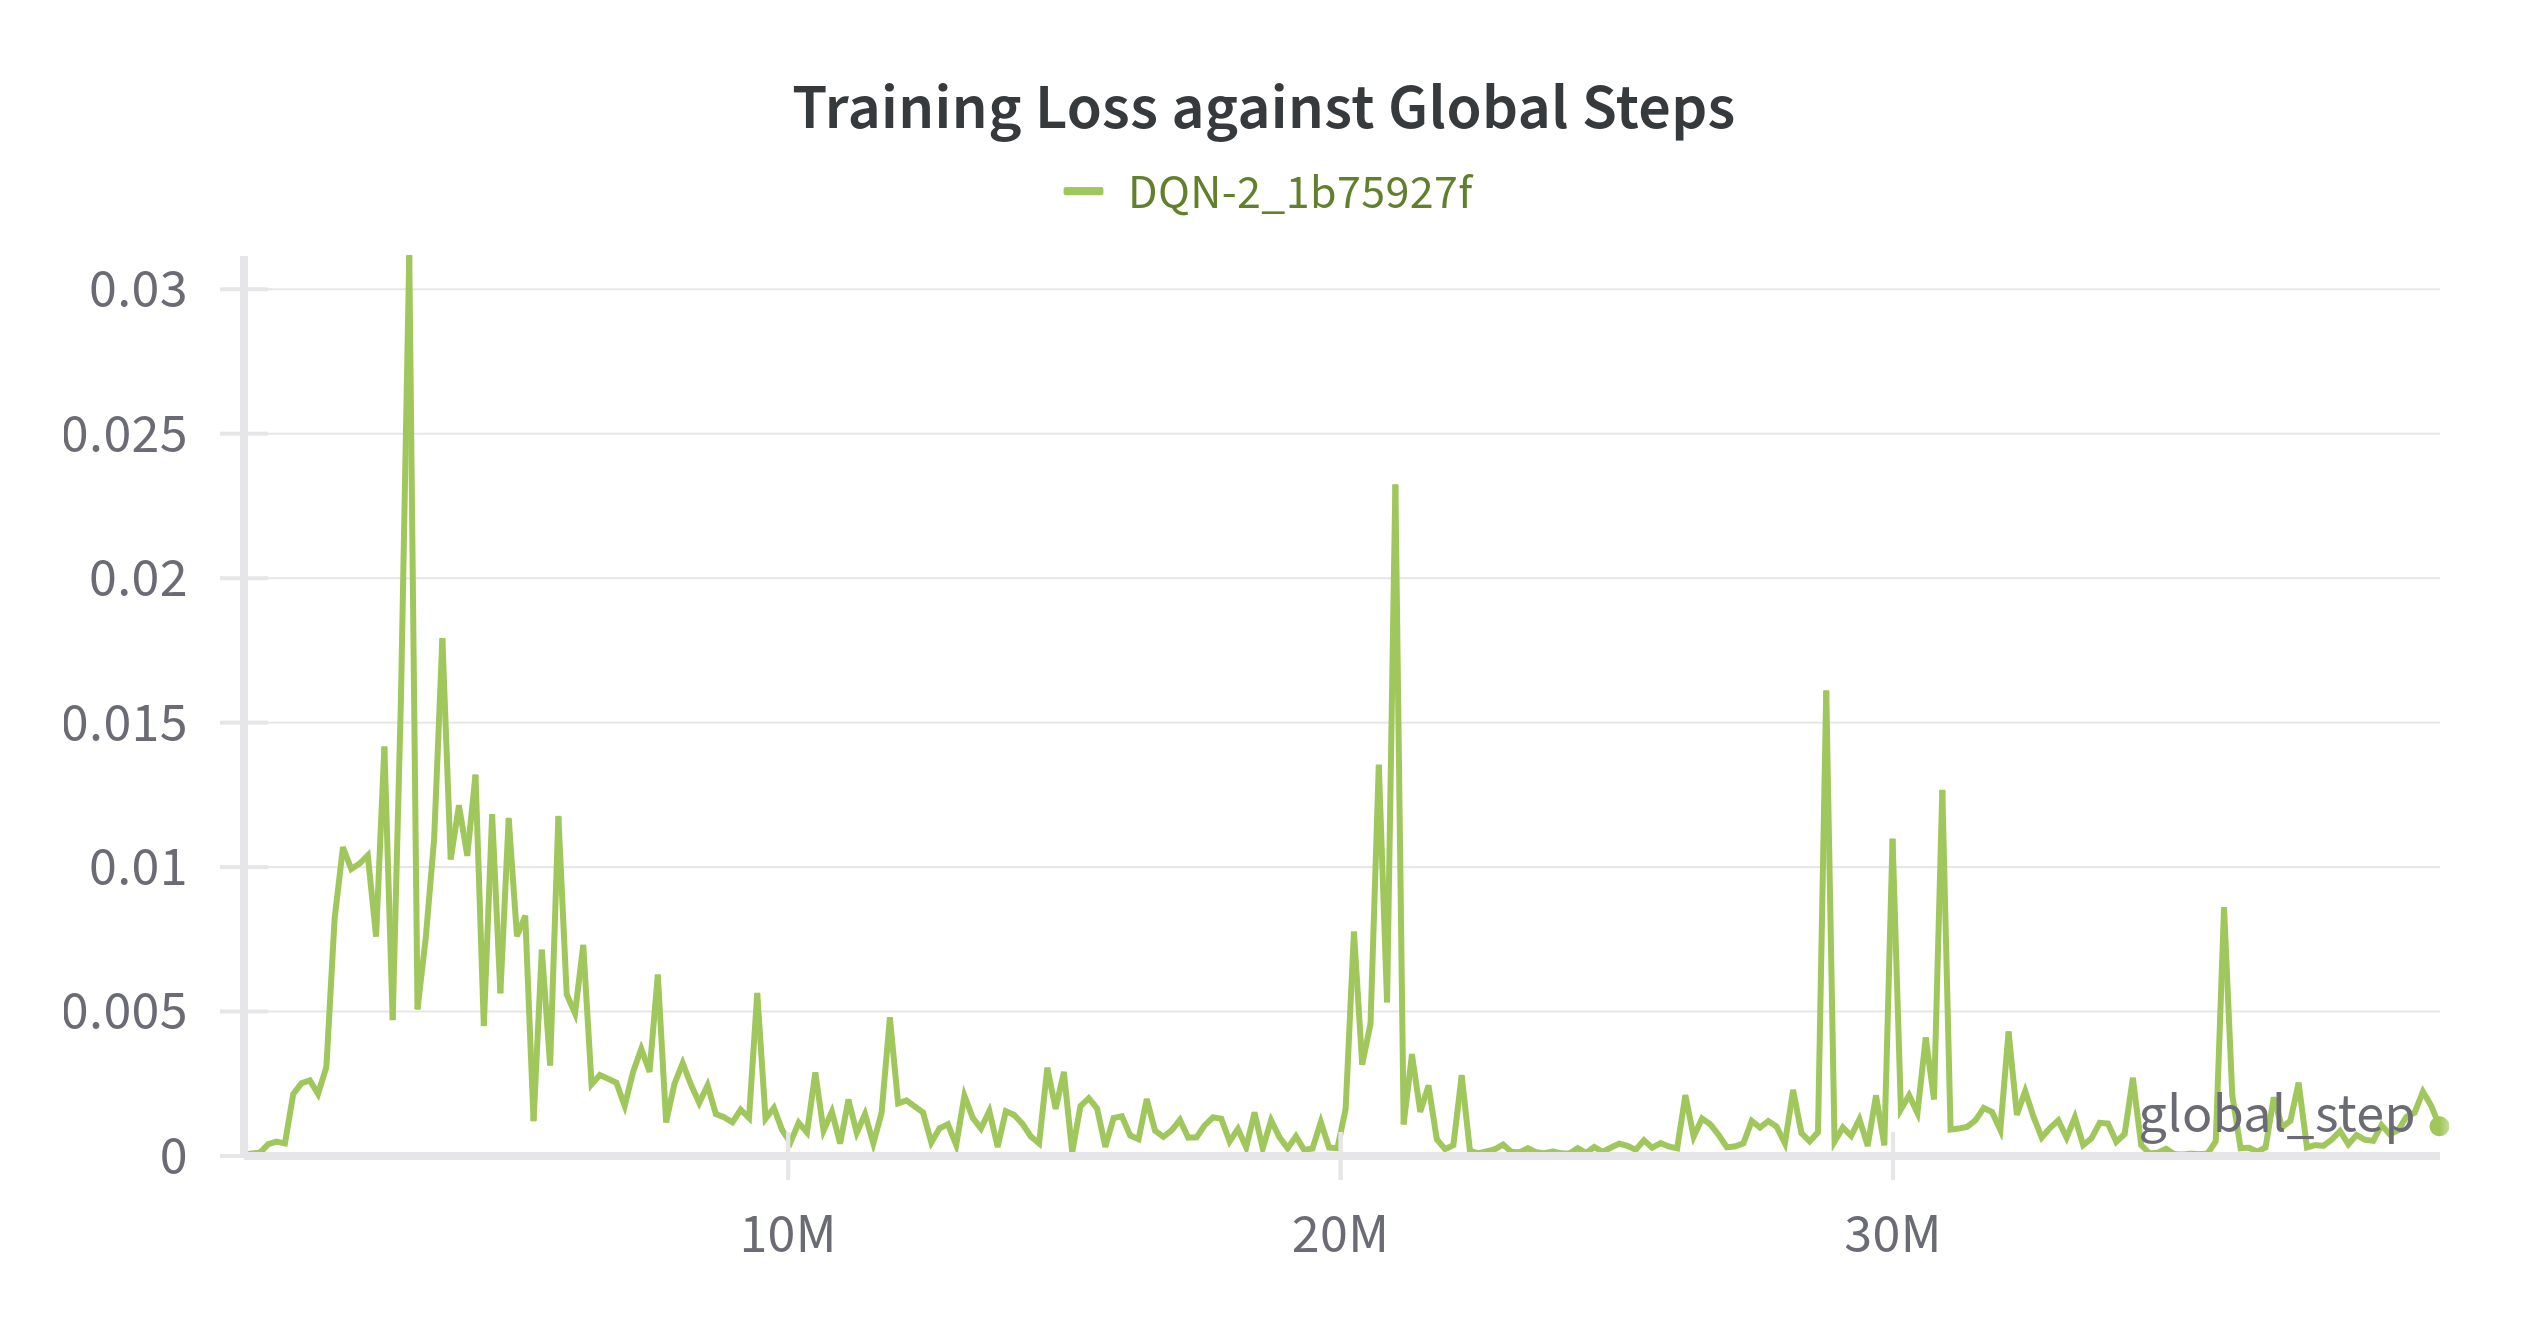
\includegraphics[width=0.49\textwidth]{figures/DQN/DQN2_Training_Loss.png}} 
    \subfigure[DQN-3]{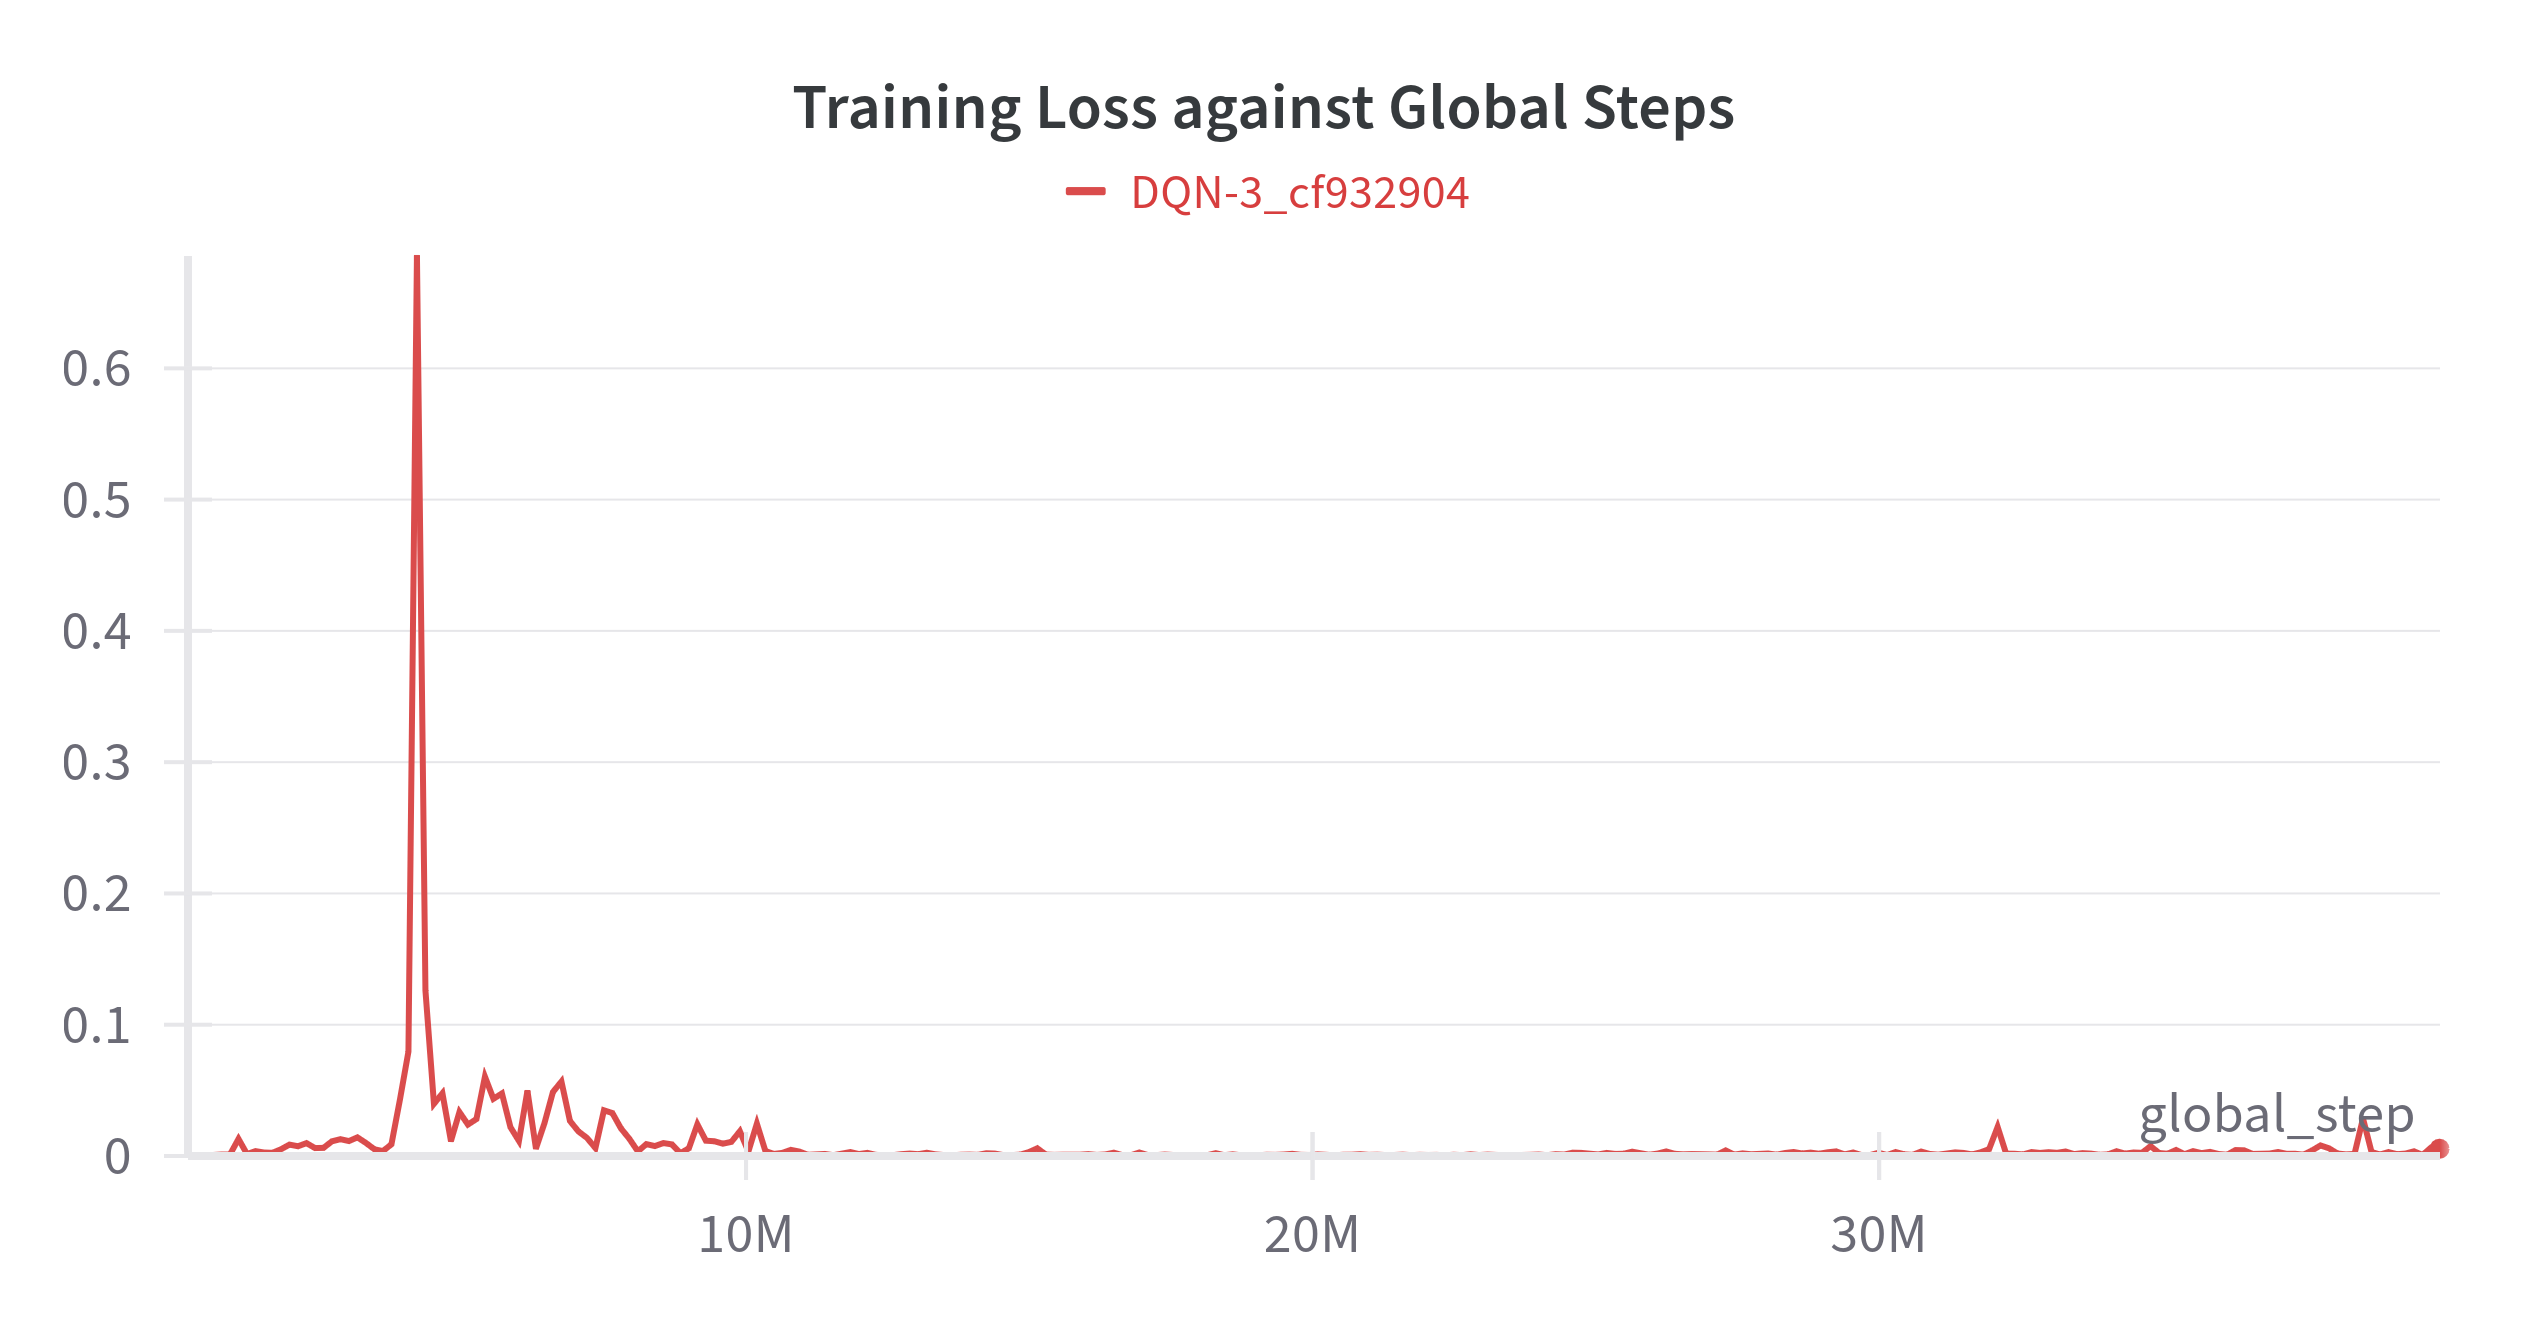
\includegraphics[width=0.49\textwidth]{figures/DQN/DQN3_Training_Loss.png}}
    \subfigure[DQN-4]{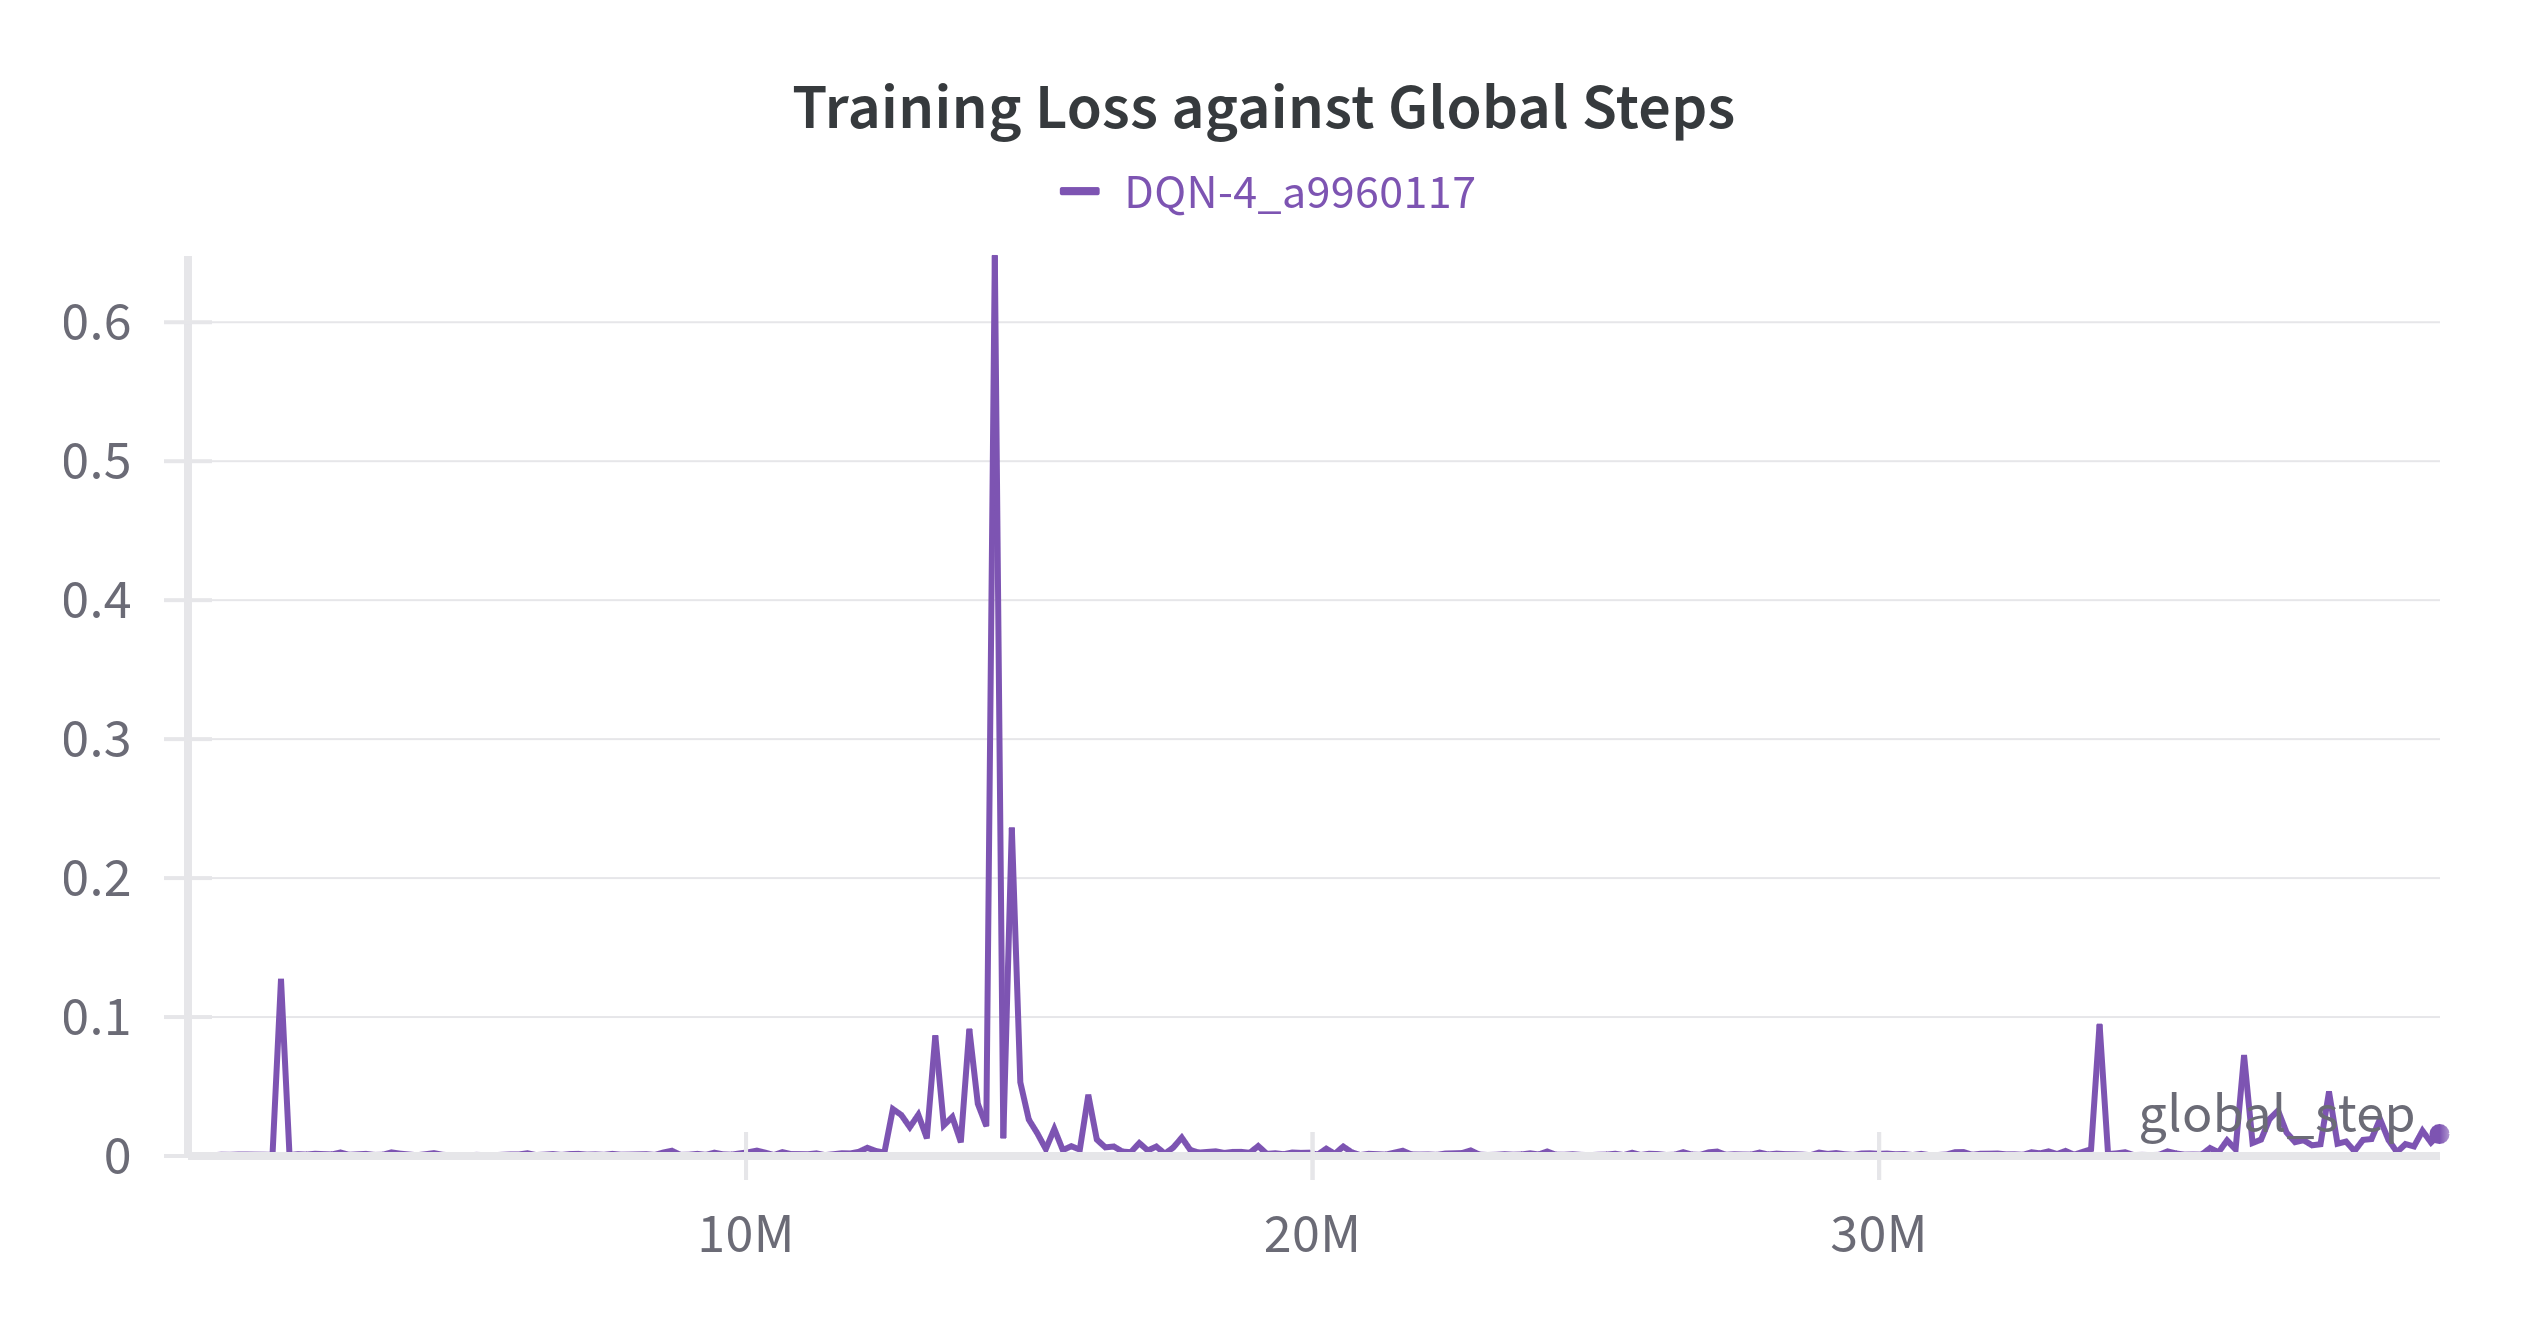
\includegraphics[width=0.49\textwidth]{figures/DQN/DQN4_Training_Loss.png}}
    \caption{Training Loss of all DQN Agents}
    \label{fig:DQN_training_loss}
\end{figure}

Figure \ref{fig:DQN_training_loss} shows the training loss of each agent and shows that all 4 agents had low loss values throughout the training. However, all had massive spikes at random intervals. Althrough, it can be said that DQN-1, DQN-3 and DQN-4 has more consistent low loss values compared to DQN-2. This suggests that DQN-2 had a more inconsistent training process compared to the other agents. This is evident from the total reward of DQN-2, which showed a more speratic amount of performance compared to the other agents.

\subsubsection*{Badge Count}

\begin{figure}[H]
    \centering
    \subfigure[DQN-1]{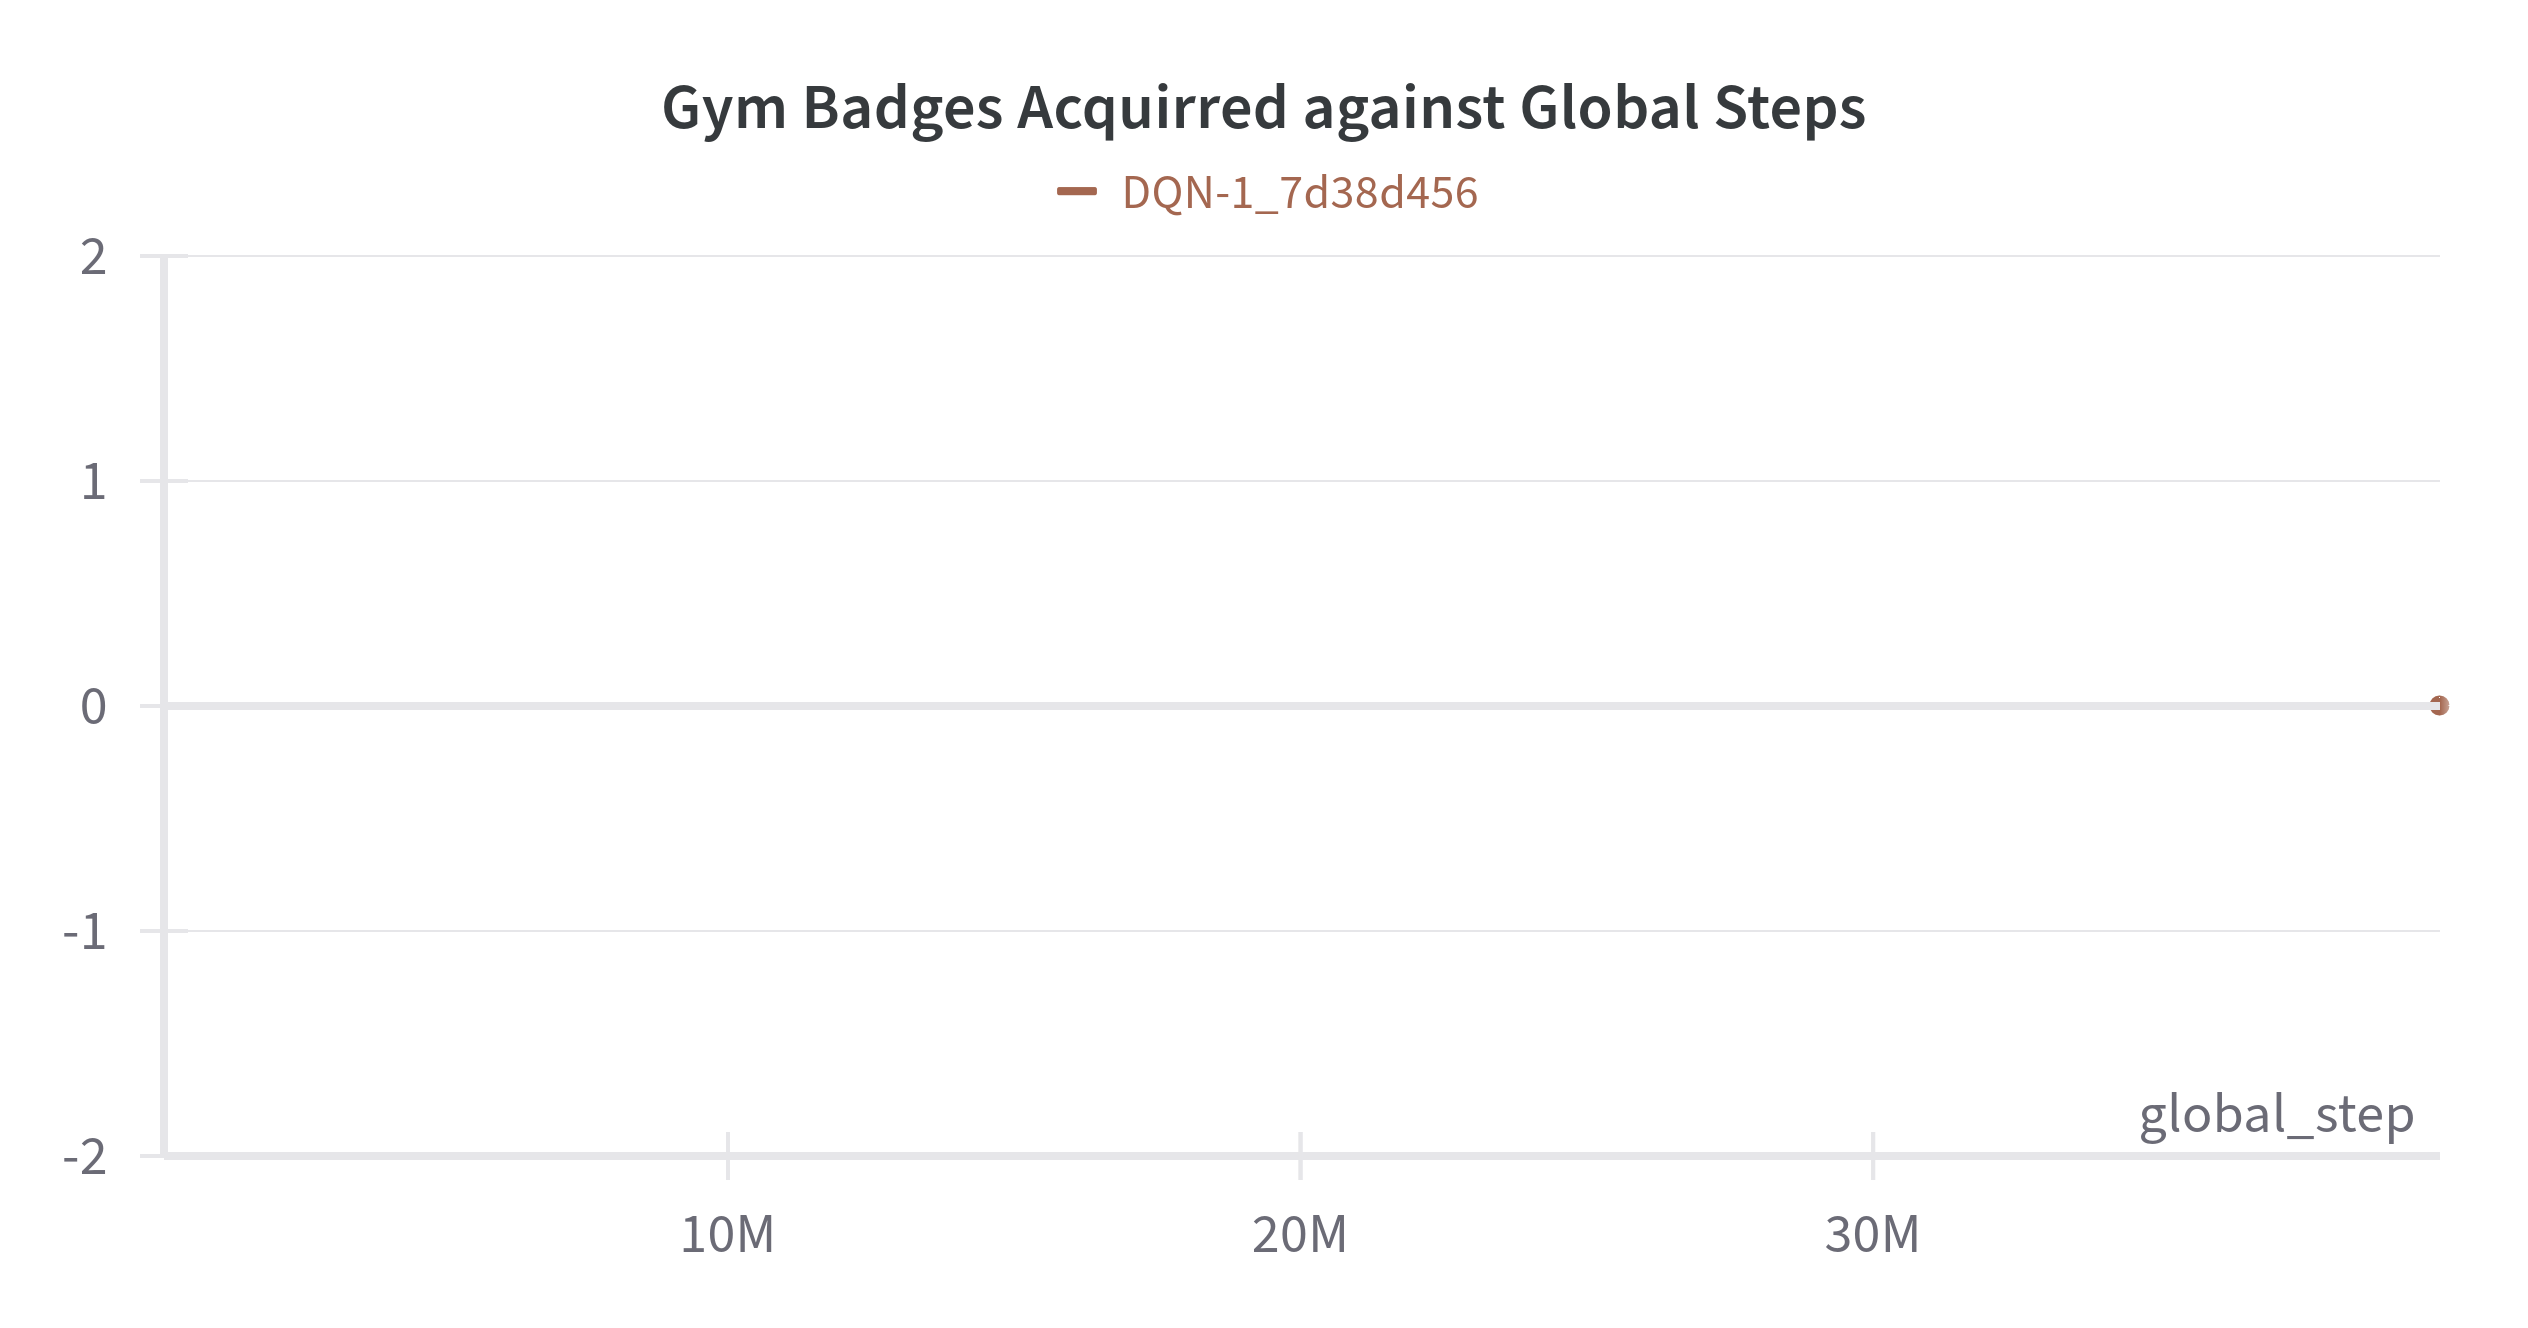
\includegraphics[width=0.49\textwidth]{figures/DQN/DQN1_Badge_Count.png}} 
    \subfigure[DQN-2]{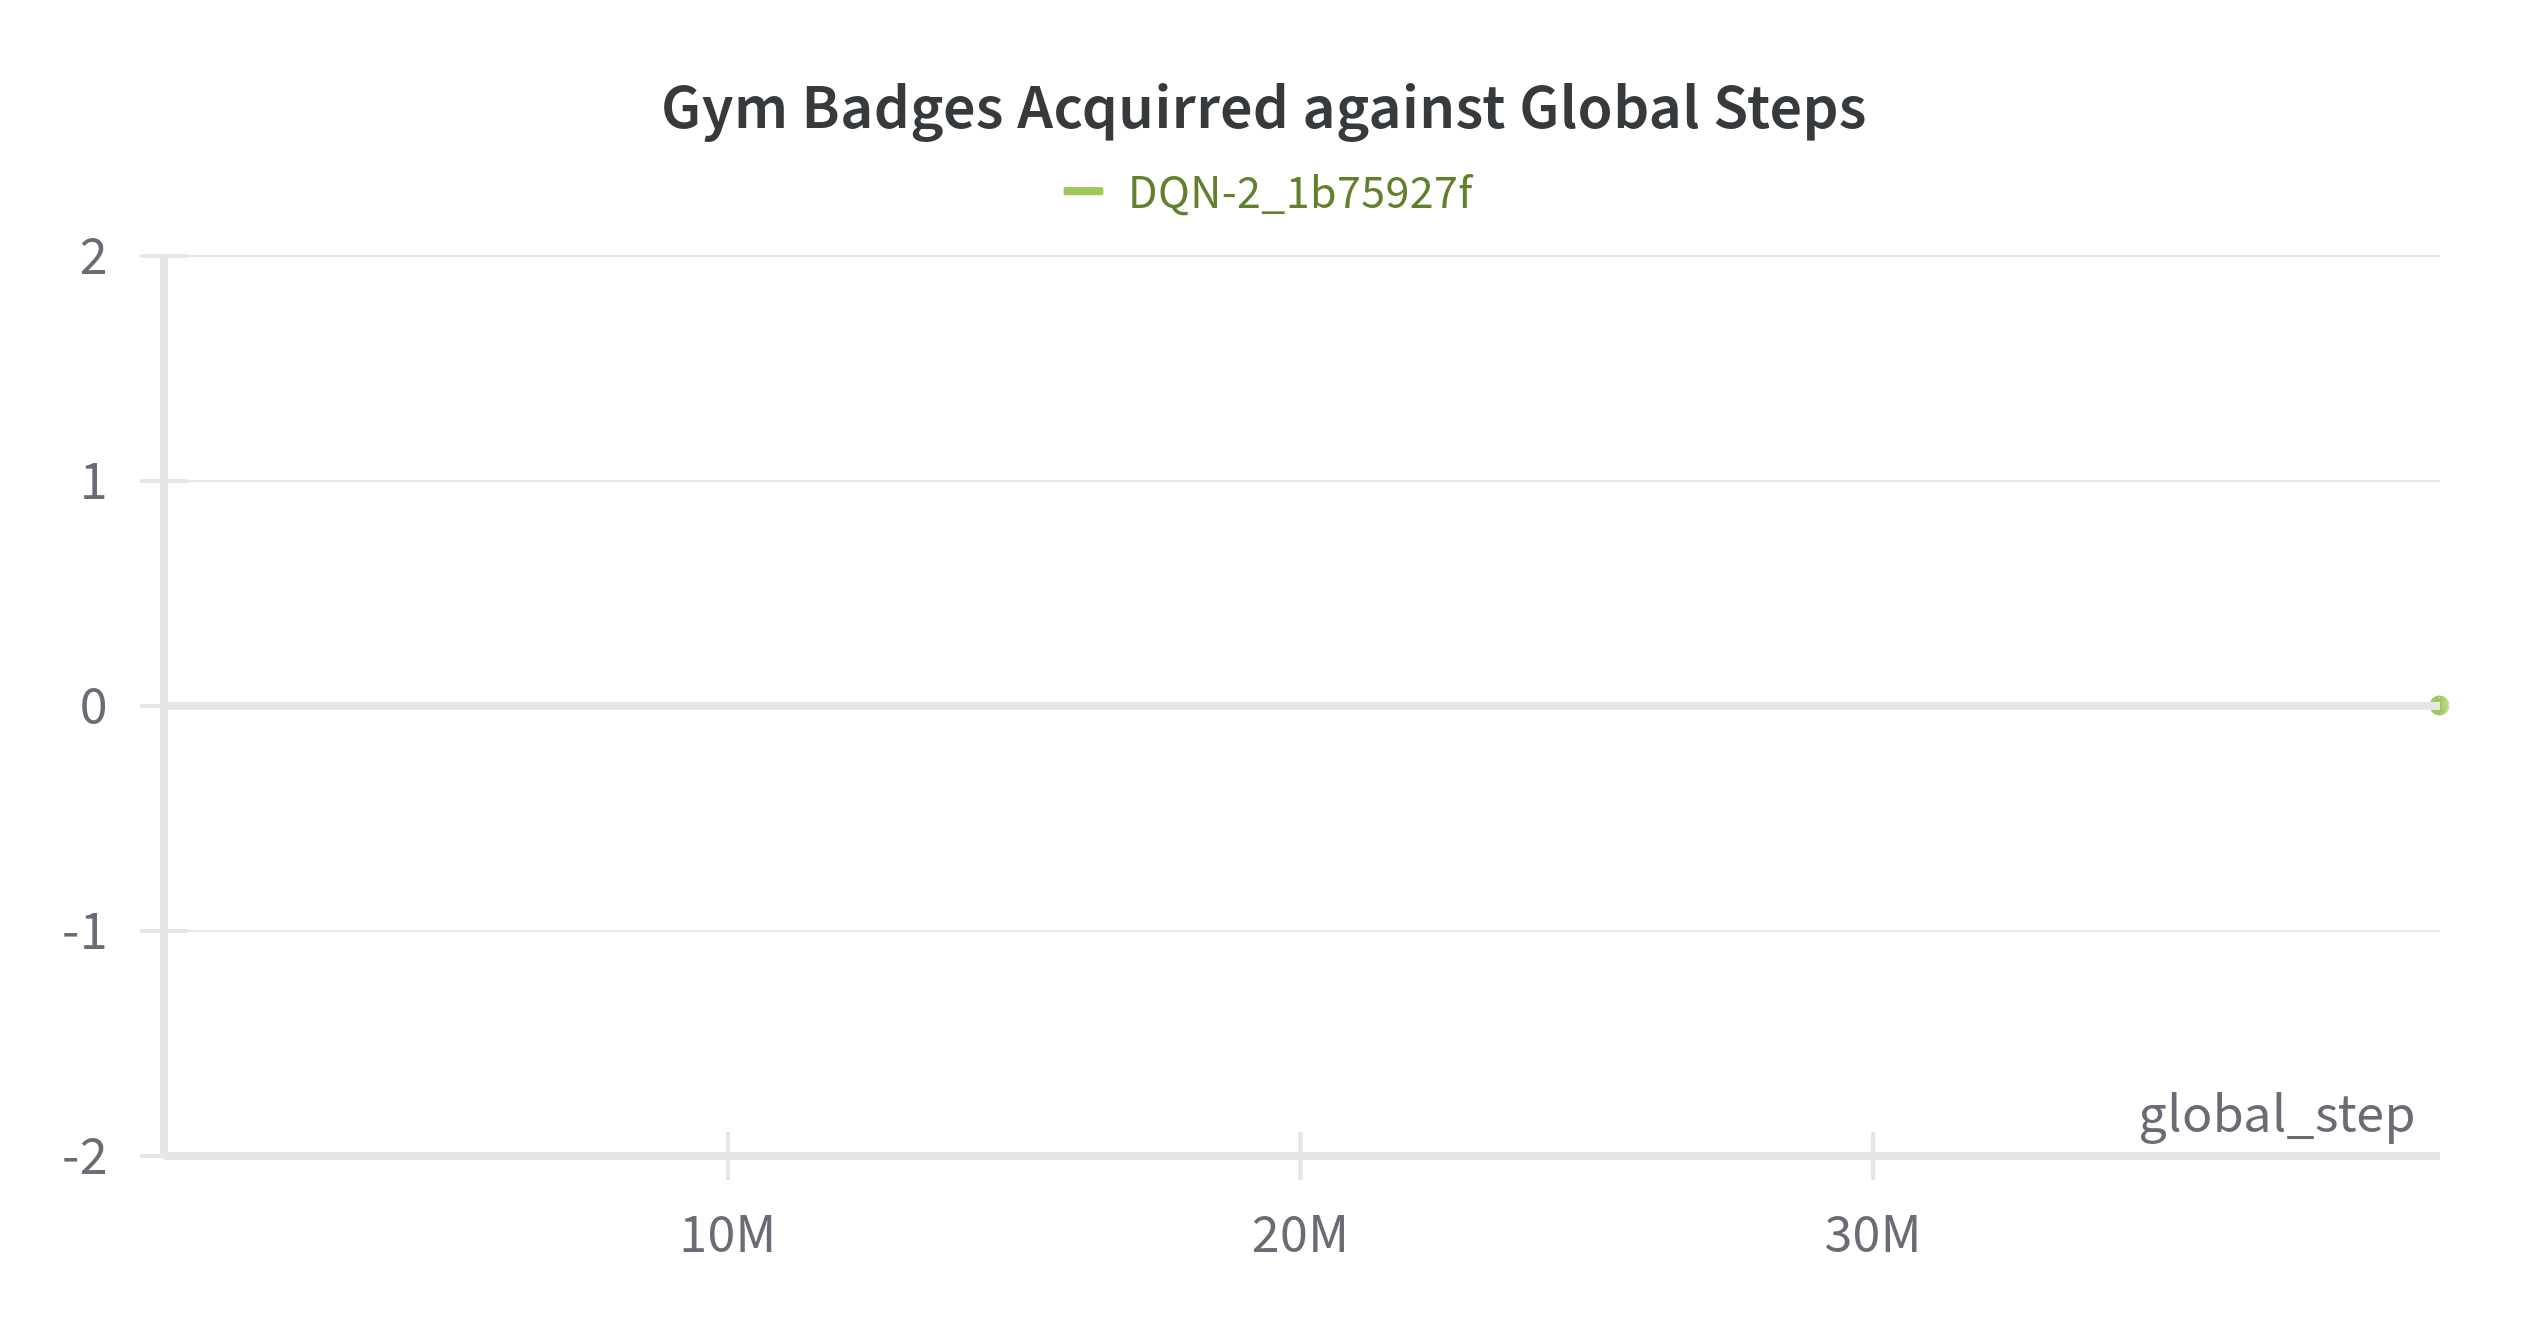
\includegraphics[width=0.49\textwidth]{figures/DQN/DQN2_Badge_Count.png}} 
    \subfigure[DQN-3]{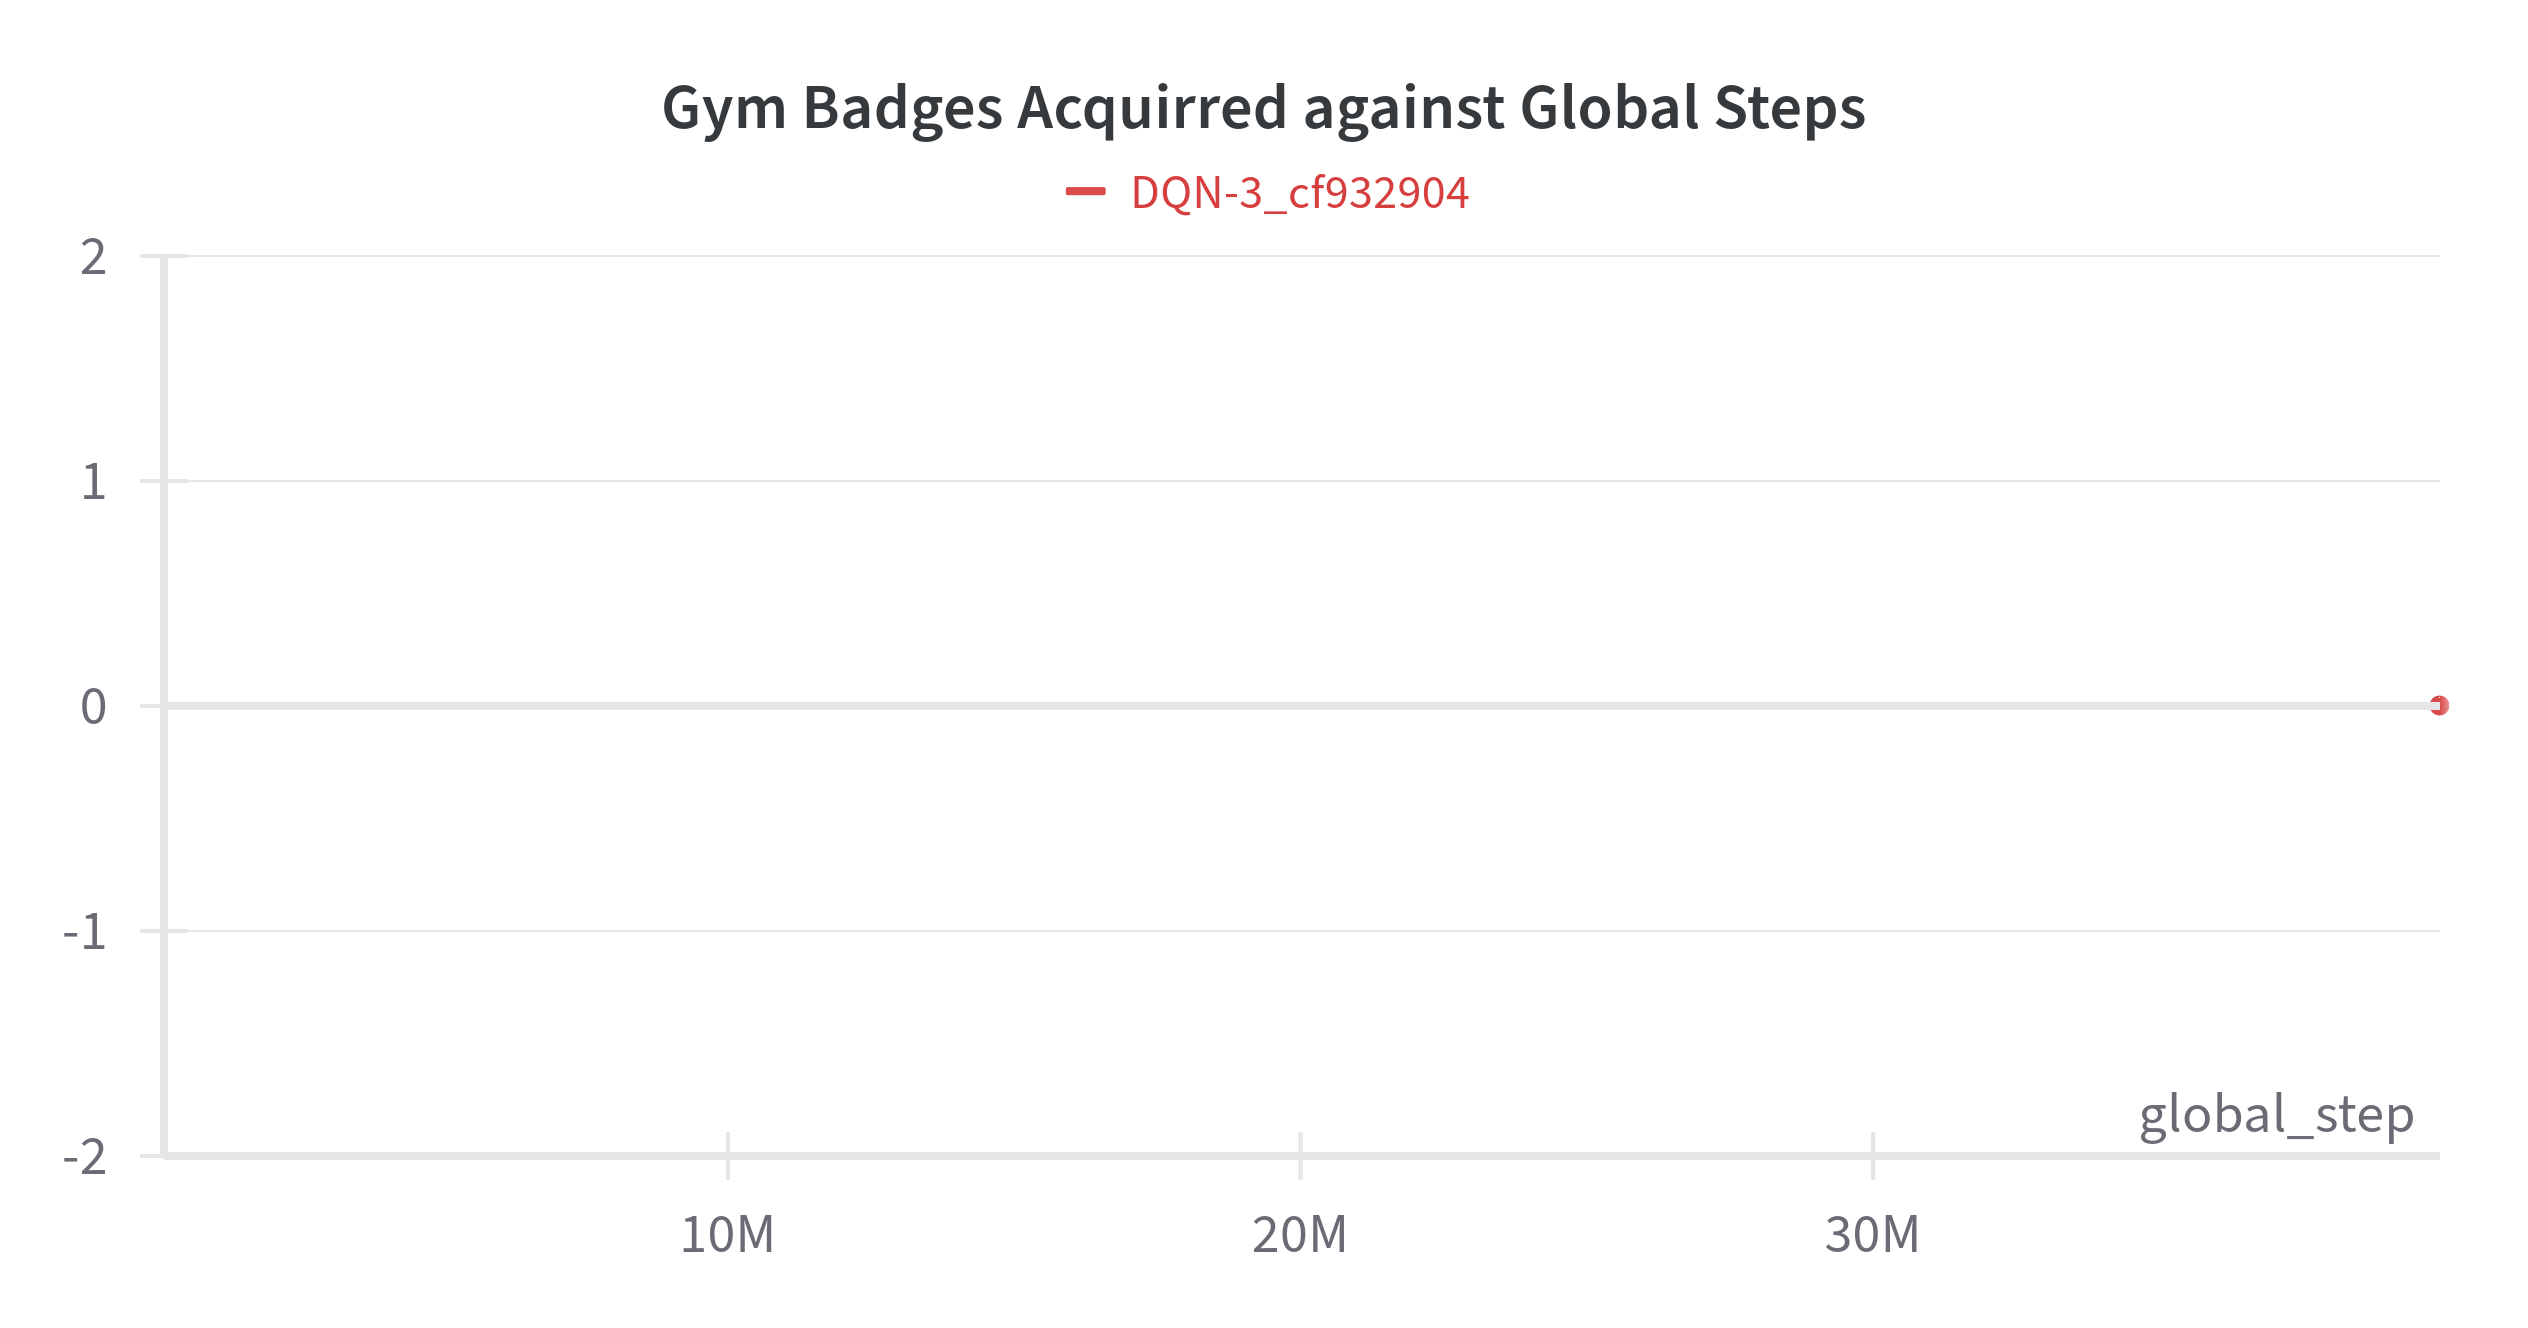
\includegraphics[width=0.49\textwidth]{figures/DQN/DQN3_Badge_Count.png}}
    \subfigure[DQN-4]{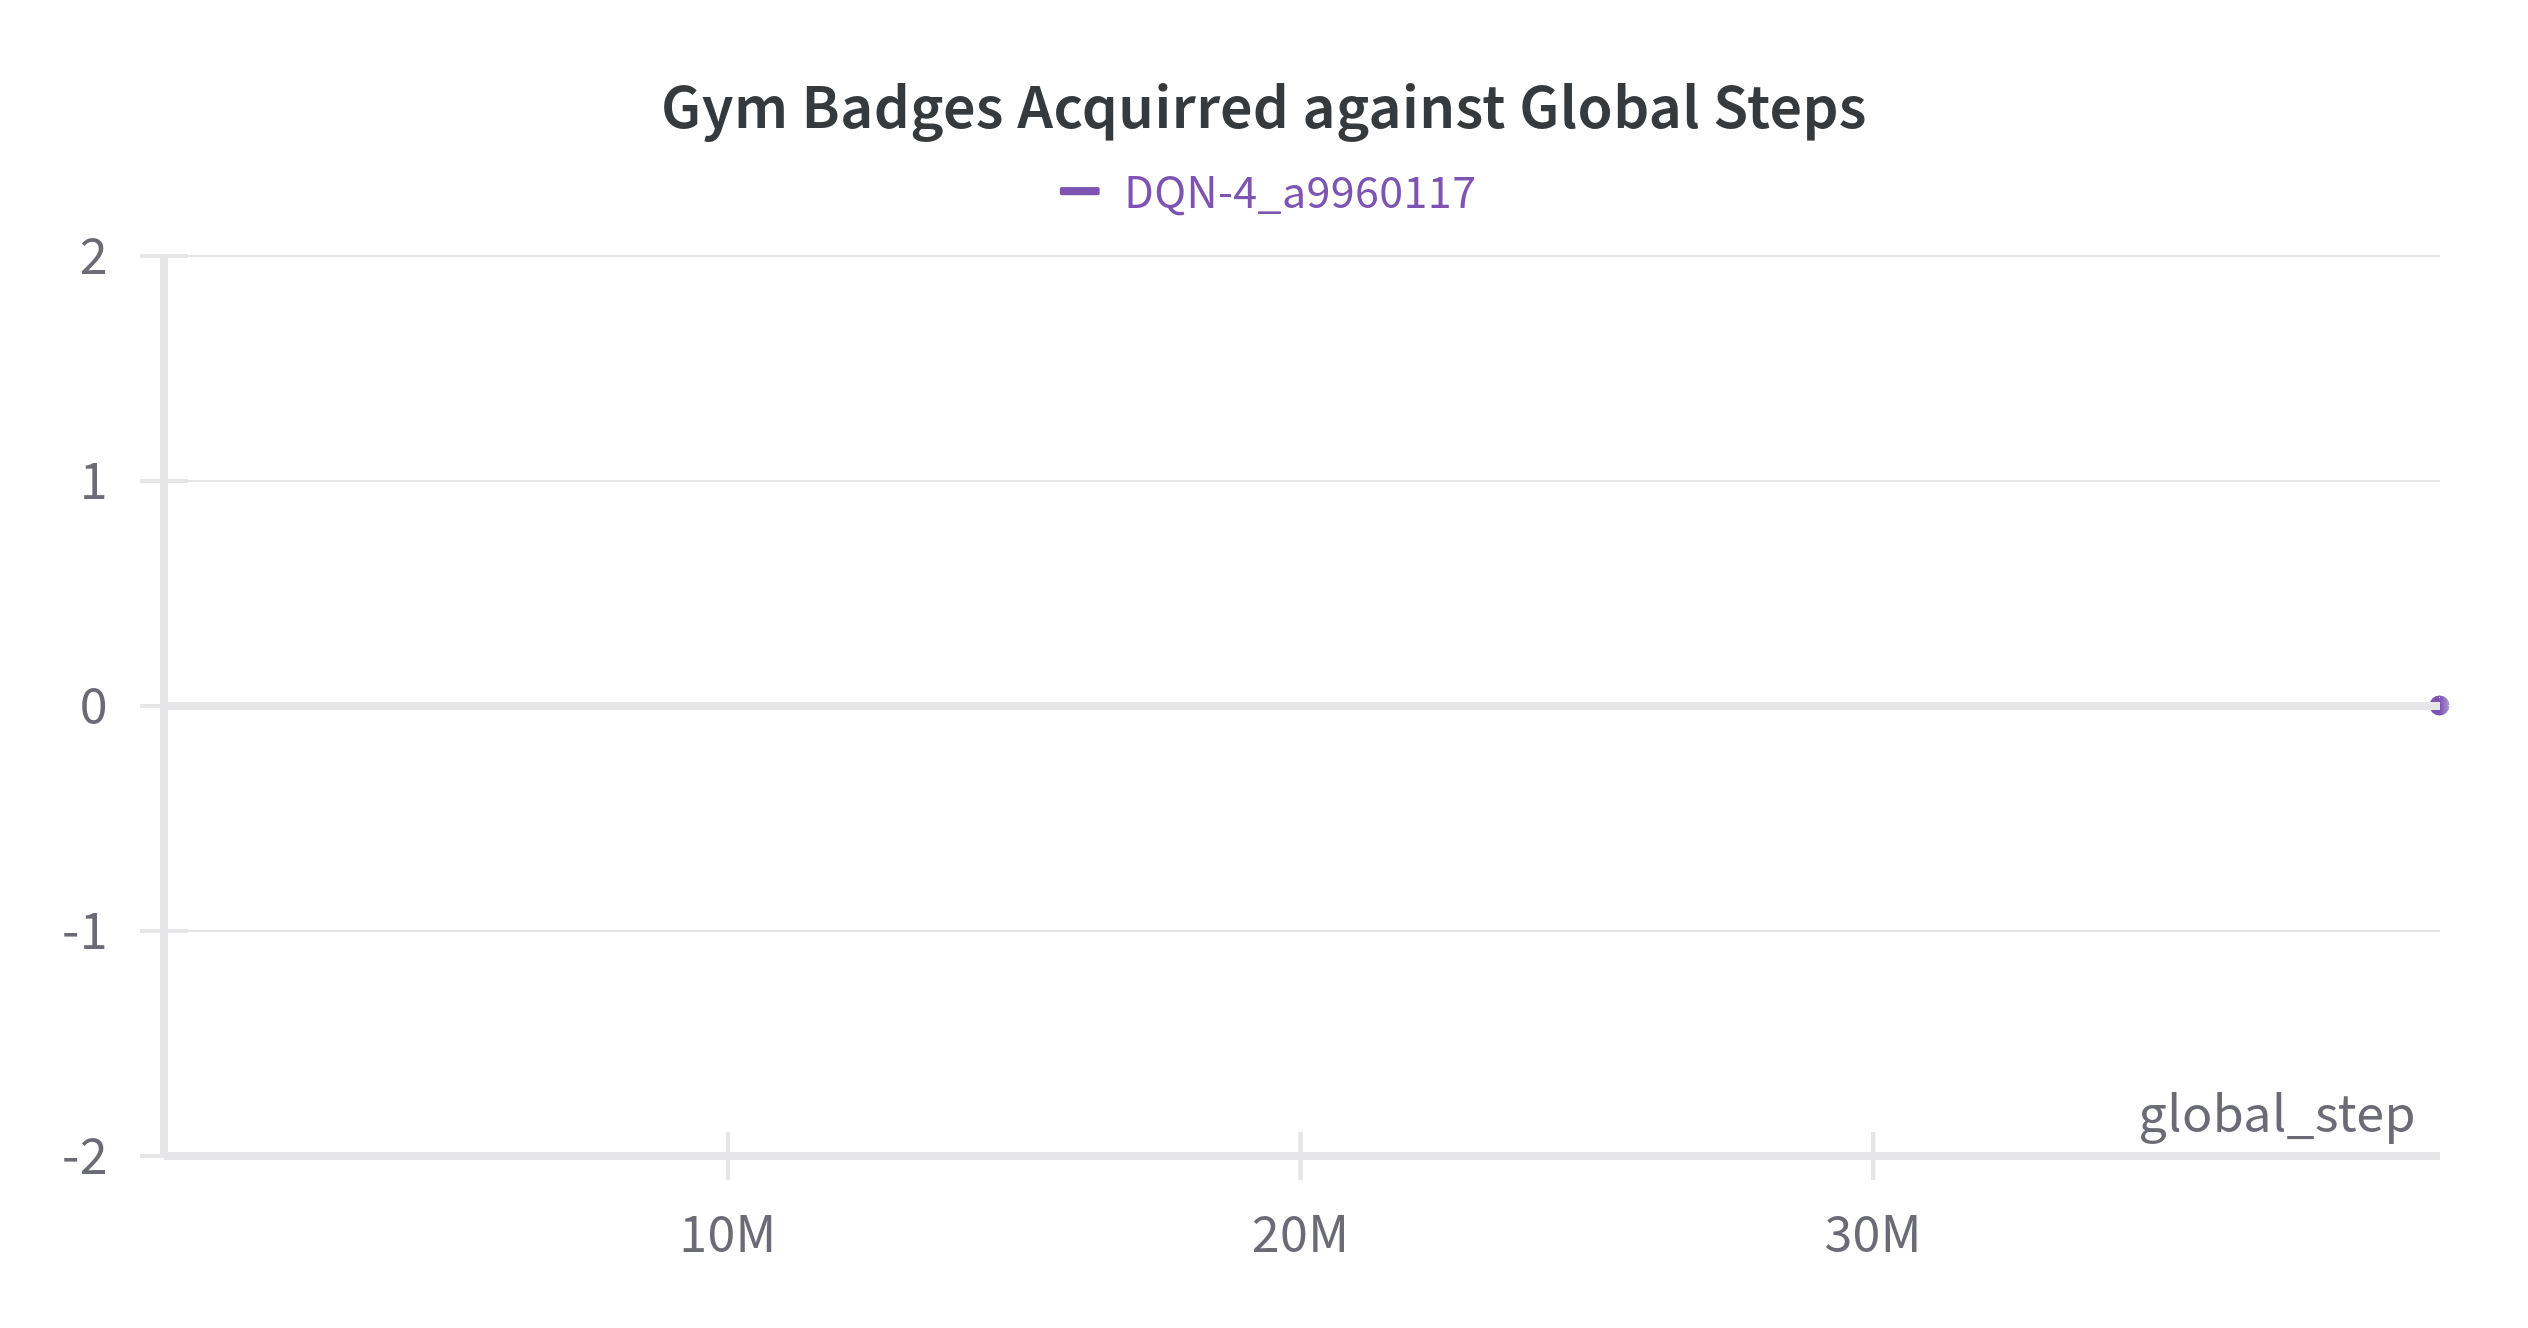
\includegraphics[width=0.49\textwidth]{figures/DQN/DQN4_Badge_Count.png}}
    \caption{Badge Count of all DQN Agents}
    \label{fig:DQN_badge_count}
\end{figure}

Figure \ref{fig:DQN_badge_count} shows the badge count of each agent and shows that none of the agents were able to collect the first badge. This suggests that the agents were not able to explore the environment effectively to reach the first gym badge. This is further confirmed by the total reward of each agent, as the difference in total reward between the start and end of training was not significant. Therefore, either value-based methods are not effective at training agents to explore multi-objective environments or the reward function was not able to guide the agents to the first gym badge.

\subsubsection*{DQN Conclusion}

In conclusion, the best performing DQN agent from the list of 4 agents is DQN-3 because of its relatively consistently high performance throughout the training. The agent showed signs of exploration at the start of training through its gradual growth in total reward throughout training. Moreover, the agent had consistently low loss values throughout training. However, the fact that DQN-3 nor the other agents were able to collect the first gym badge suggests that the agents were not able to explore the environment effectively to reach the first gym badge. This suggests that the reward function was not able to guide the agents to the first gym badge and DQN is not an effective algorithm for multi-objective RL.

\subsection{QR-DQN}

\begin{center}
    \begin{tabular}{ |c|c| } 
     \hline
     Hyperparameter & Value \\ 
     \hline
     Total Timesteps & 39,996,000 \\
     Number of Episodes &  3,333 \\
     Episode Length & 1,500 \\ 
     Parallel Instances & 8 \\
     Policy Model & MultiInputPolicy \\
     Gamma & 0.99 \\  
     Batch Size & 32 \\
     \hline
    \end{tabular}
    \end{center}

The training script used to train all 4 agents can be found within the research paper's GitHub repository under ``run\_baseline\_QRDQN.py''. A total of 8 parallel instances of the environment was trained at the same time to train for 3,333 episodes total, where each episode is 1,500 steps long. This totals up to 39,996,000 steps in total. The performance of the 4 agents can be seen on figure \ref{fig:QRDQN_total_reward} . 

\subsubsection*{Total Reward}

\begin{figure}[H]
    \centering
    \subfigure[QRDQN-1]{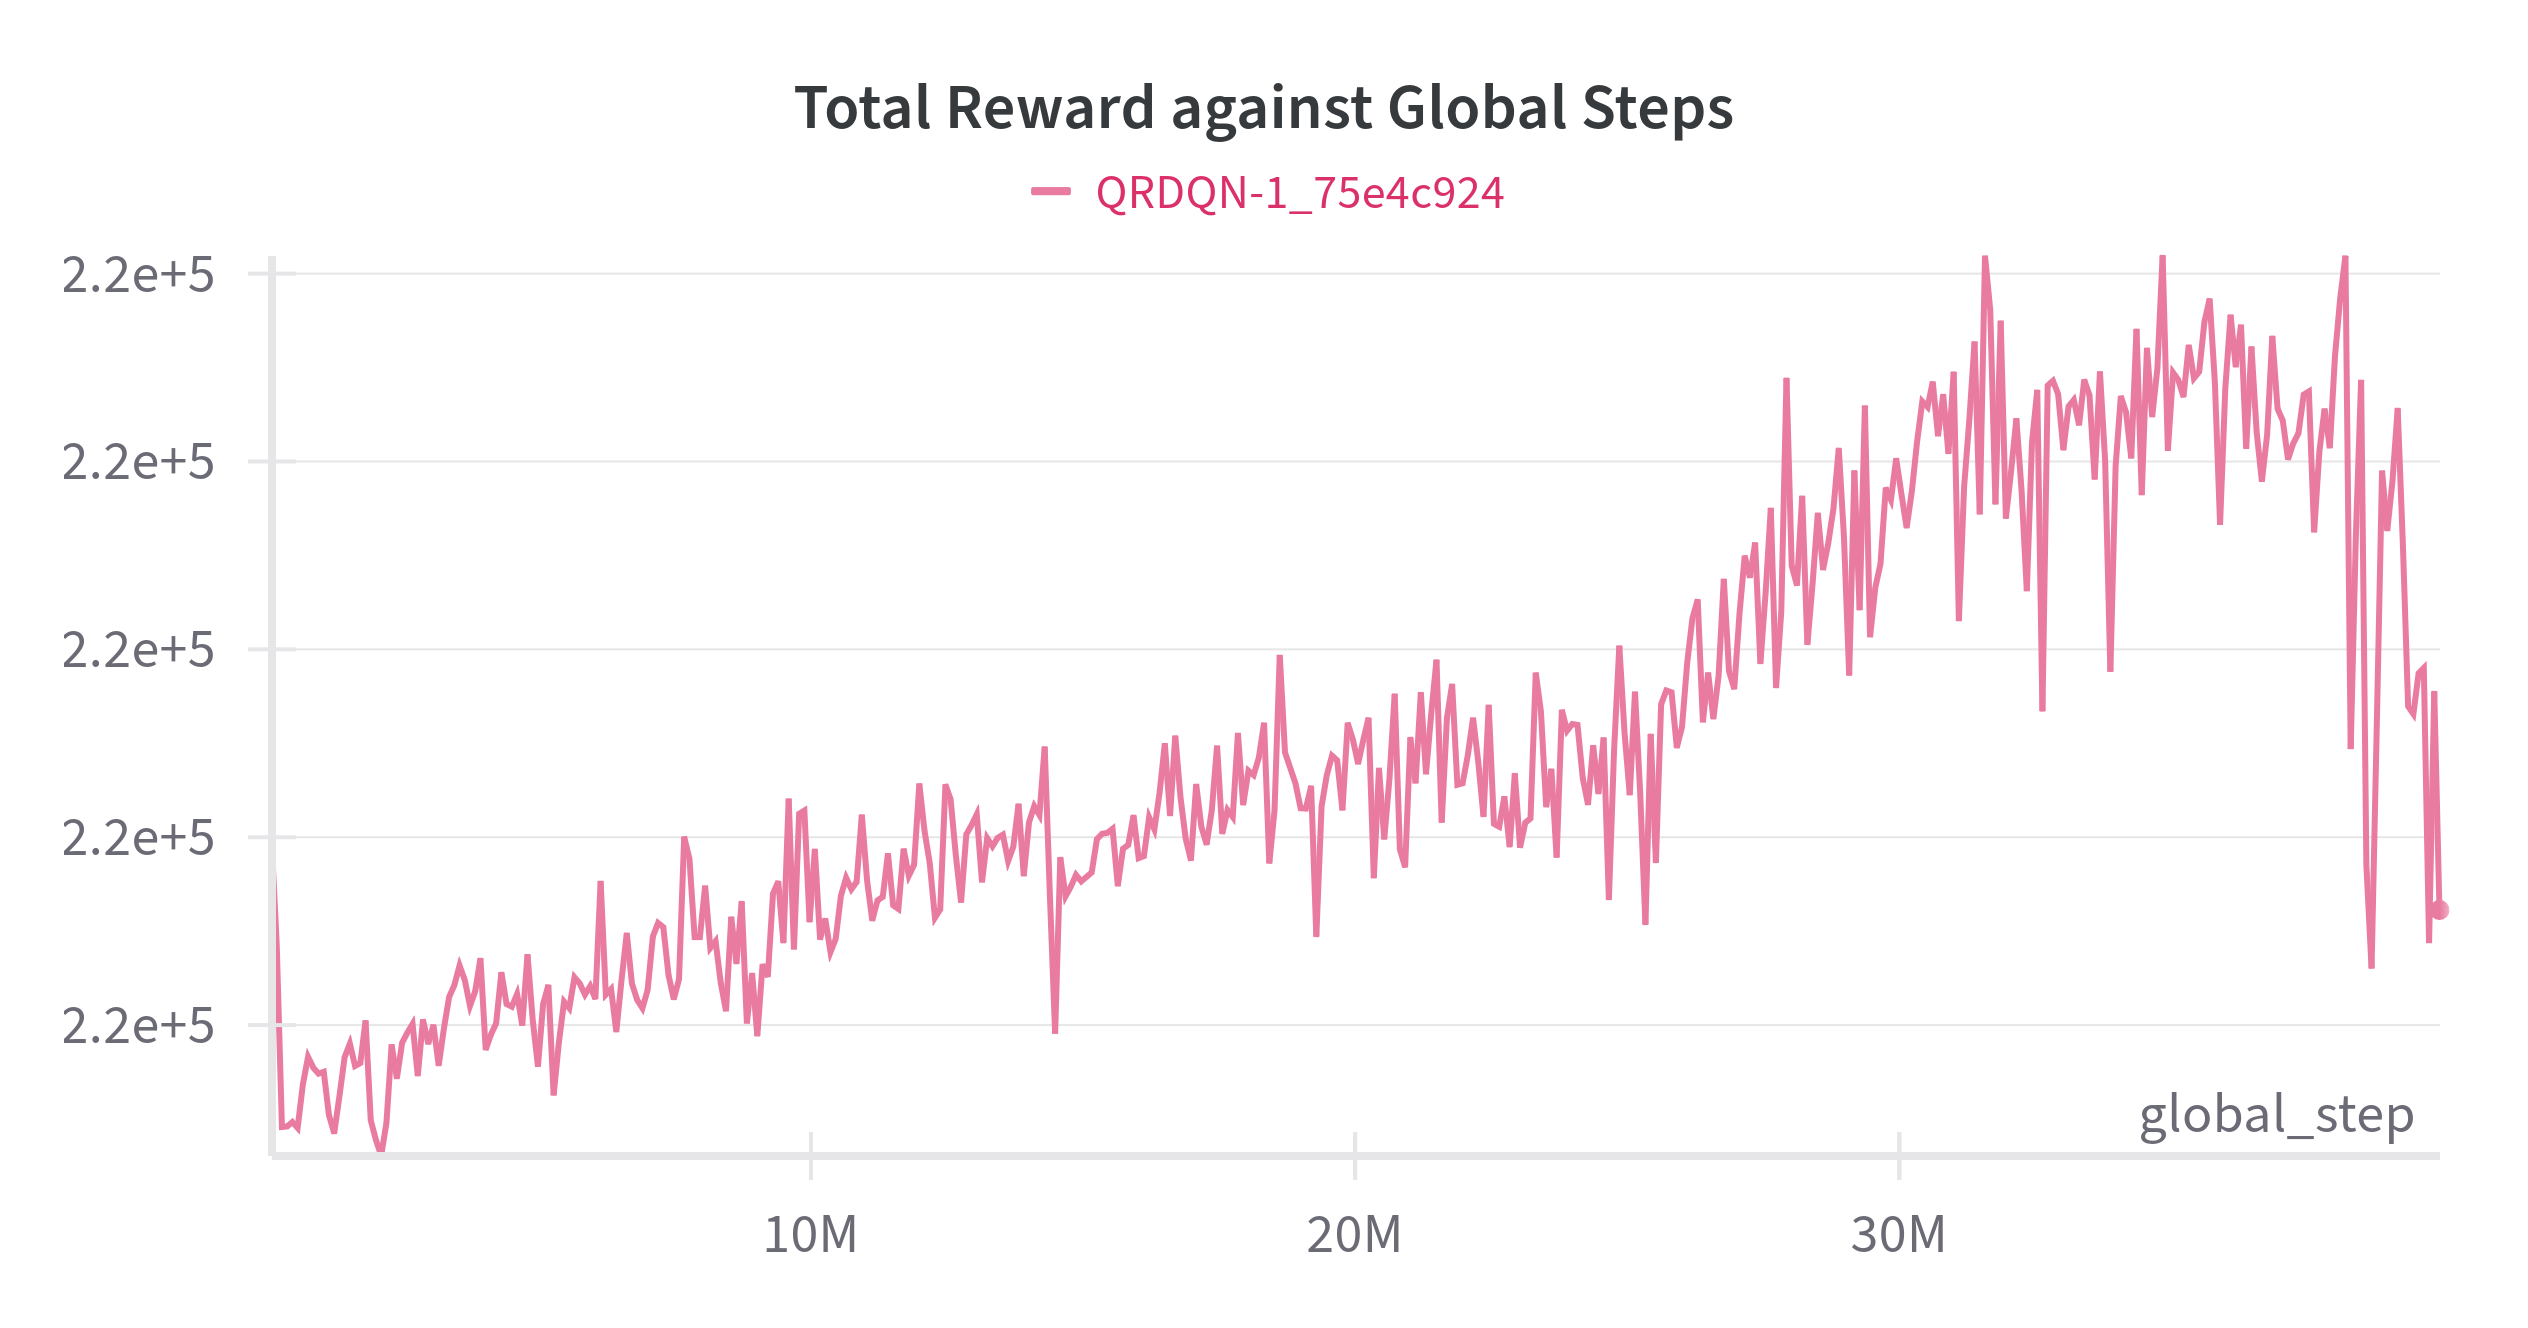
\includegraphics[width=0.49\textwidth]{figures/QRDQN/QRDQN1_Total_Reward.png}} 
    \subfigure[QRDQN-2]{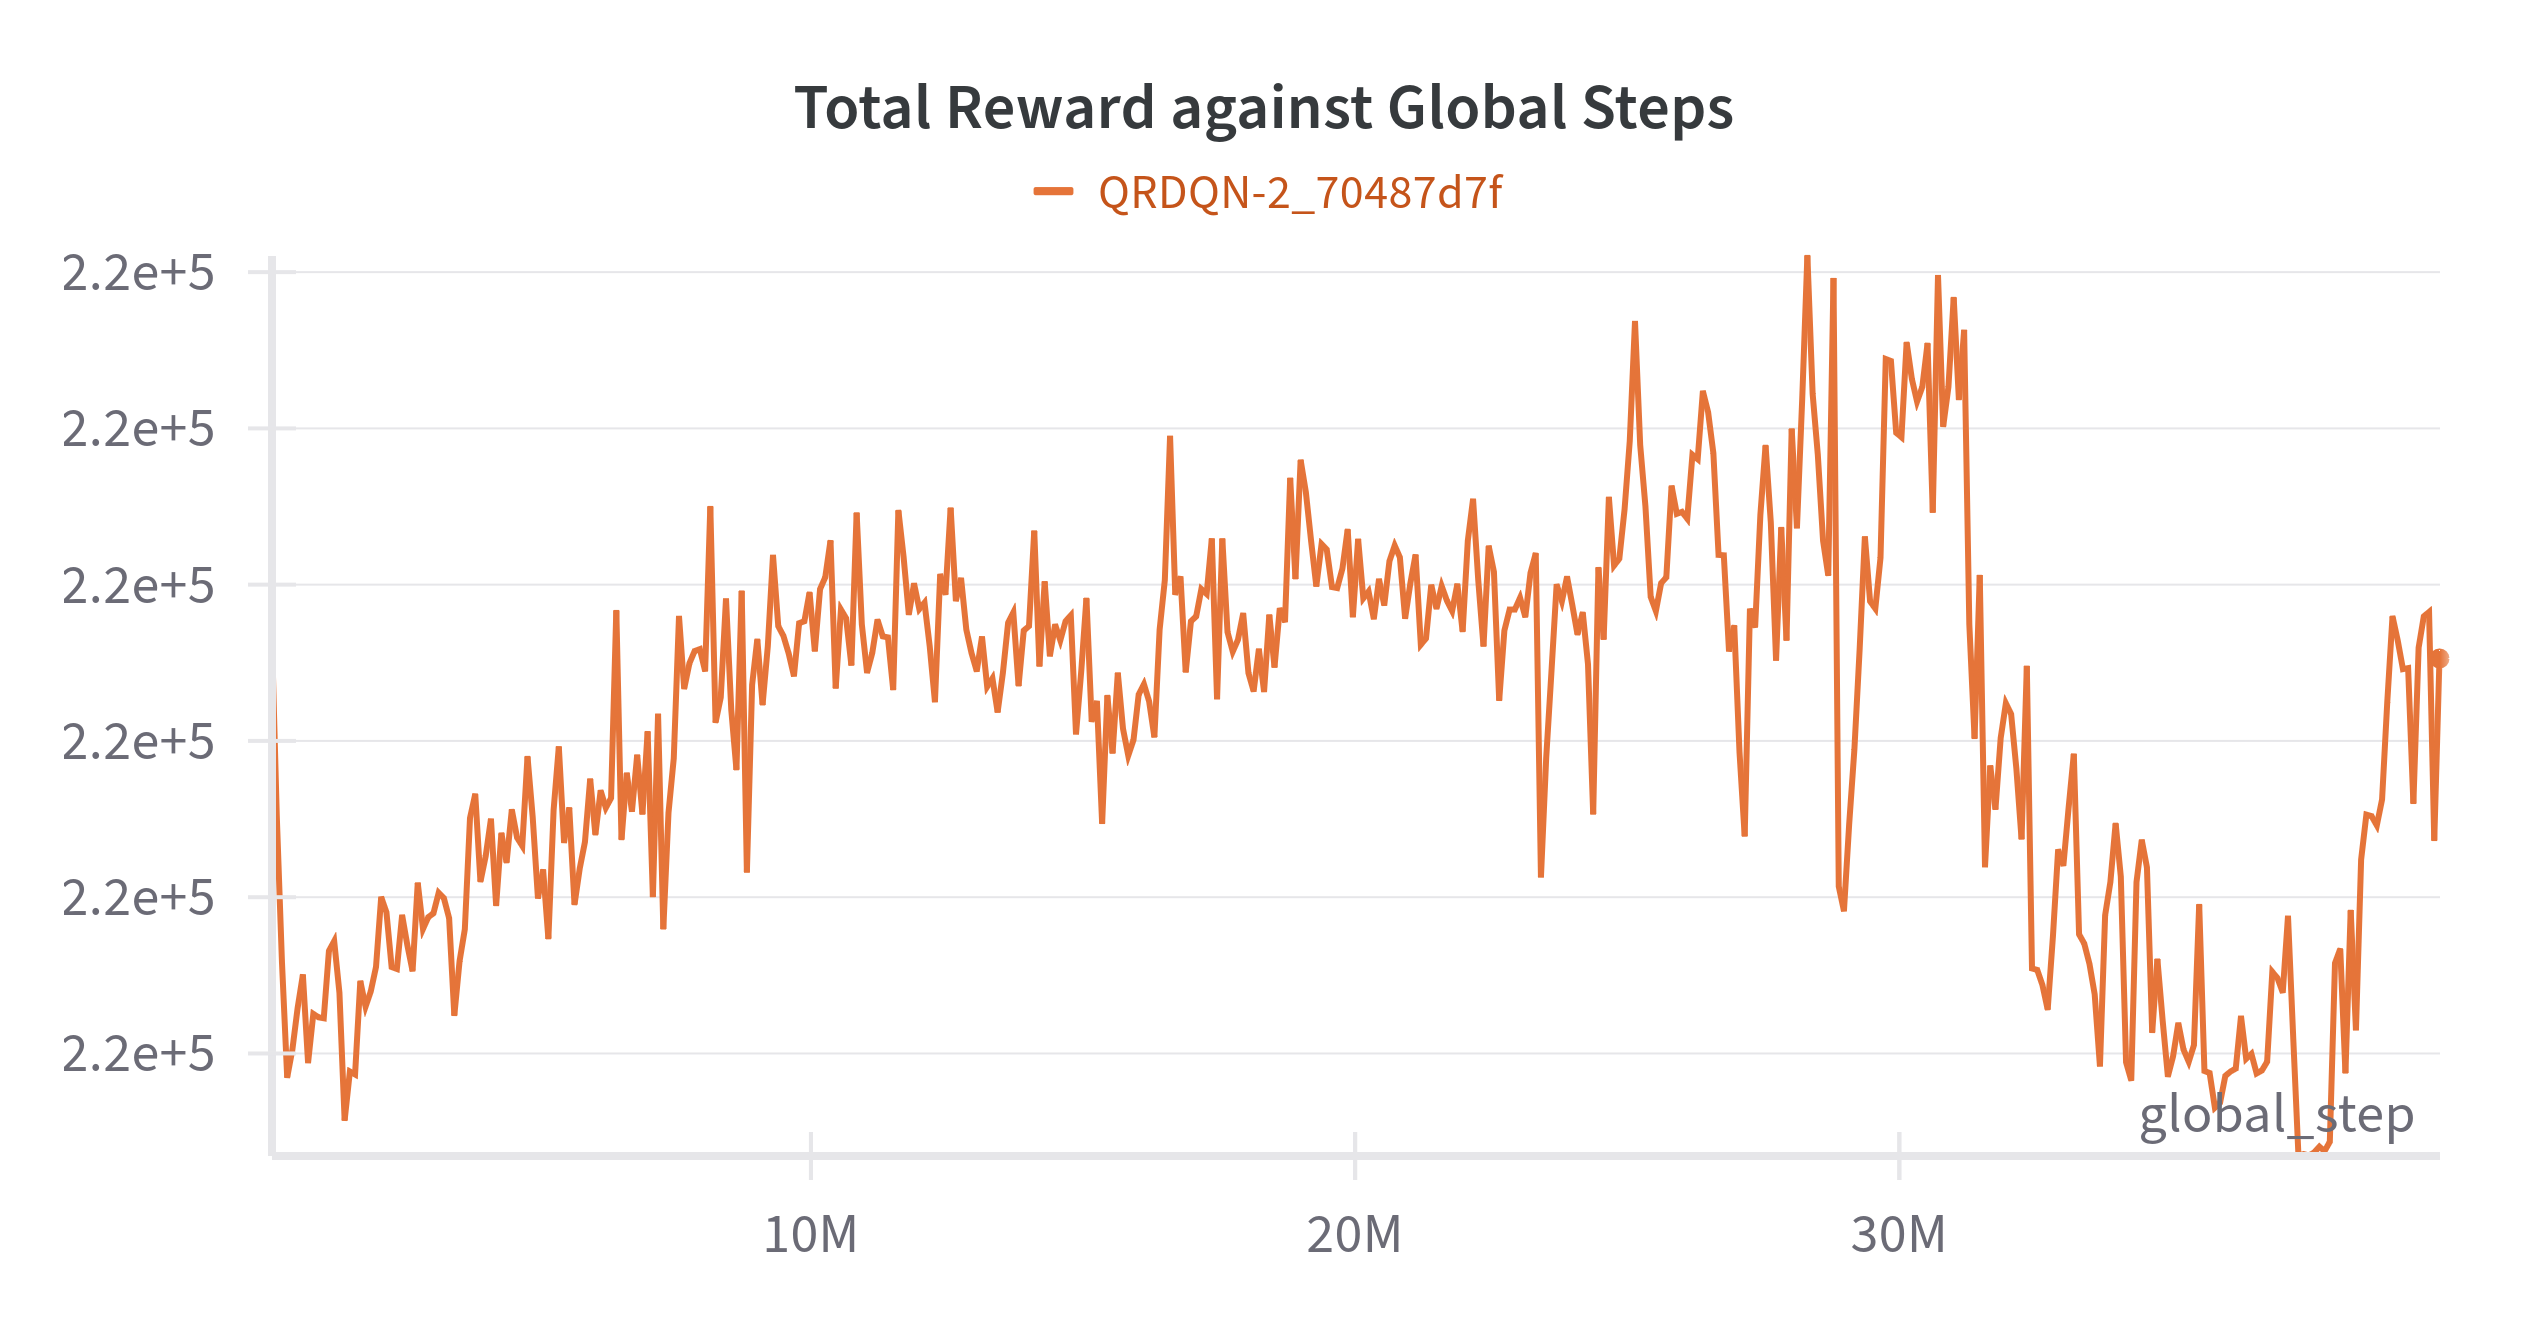
\includegraphics[width=0.49\textwidth]{figures/QRDQN/QRDQN2_Total_Reward.png}} 
    \subfigure[QRDQN-3]{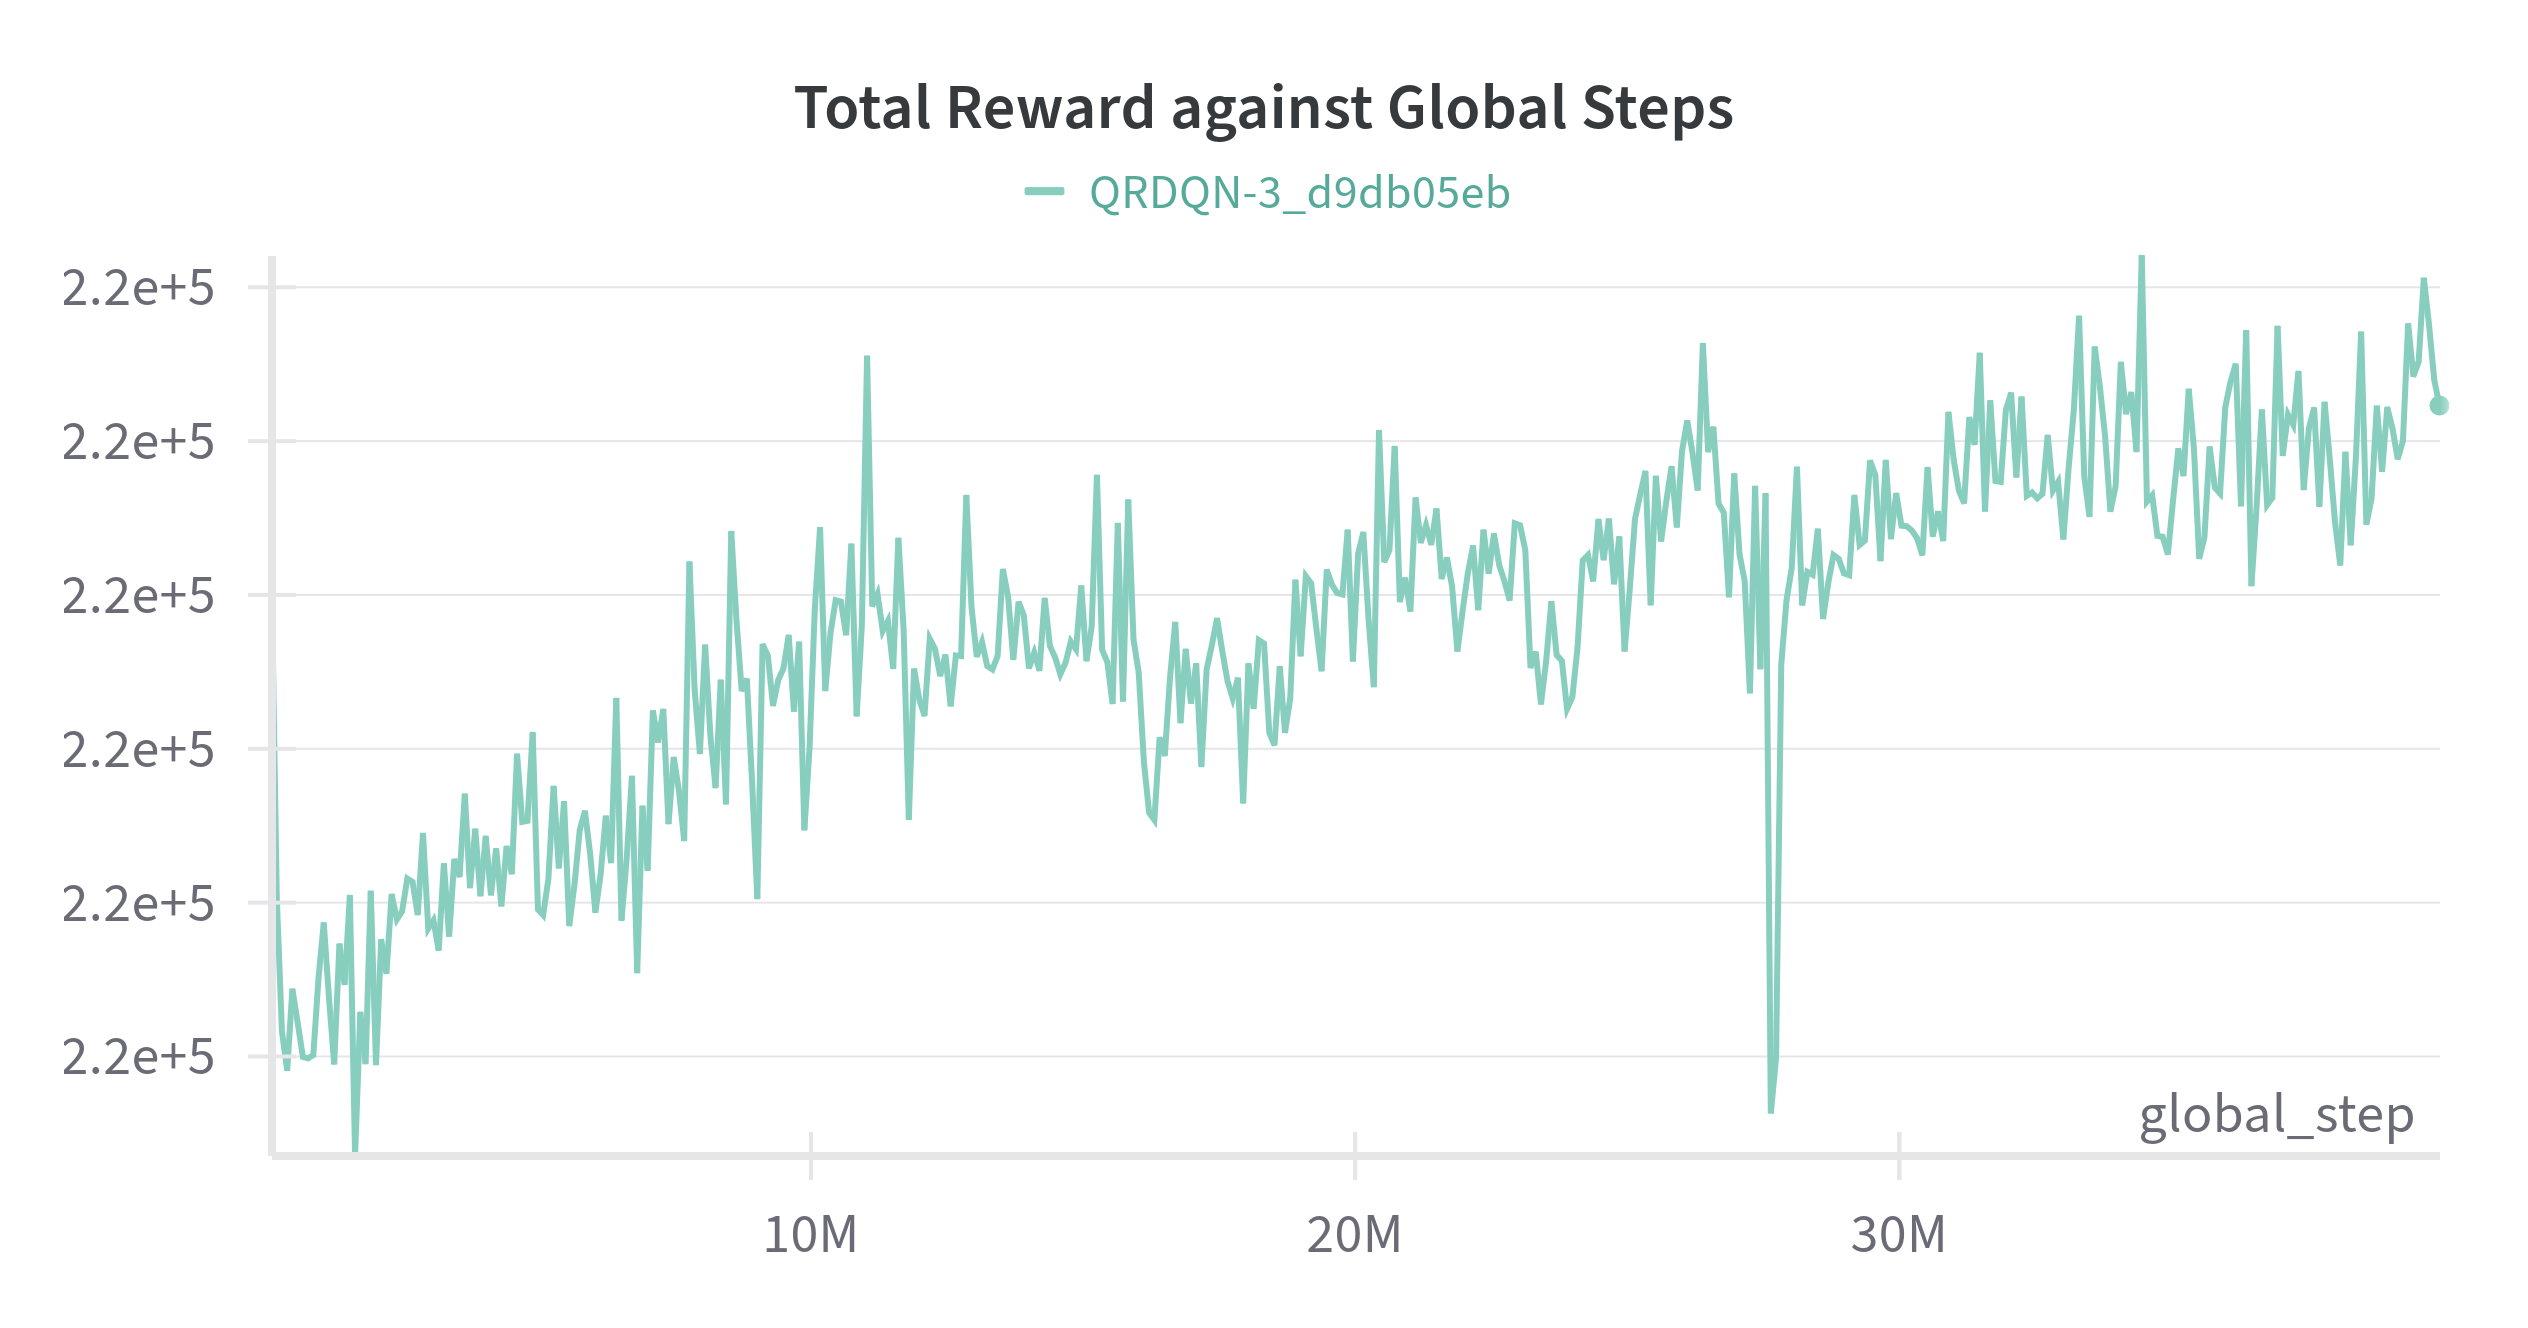
\includegraphics[width=0.49\textwidth]{figures/QRDQN/QRDQN3_Total_Reward.png}}
    \subfigure[QRDQN-4]{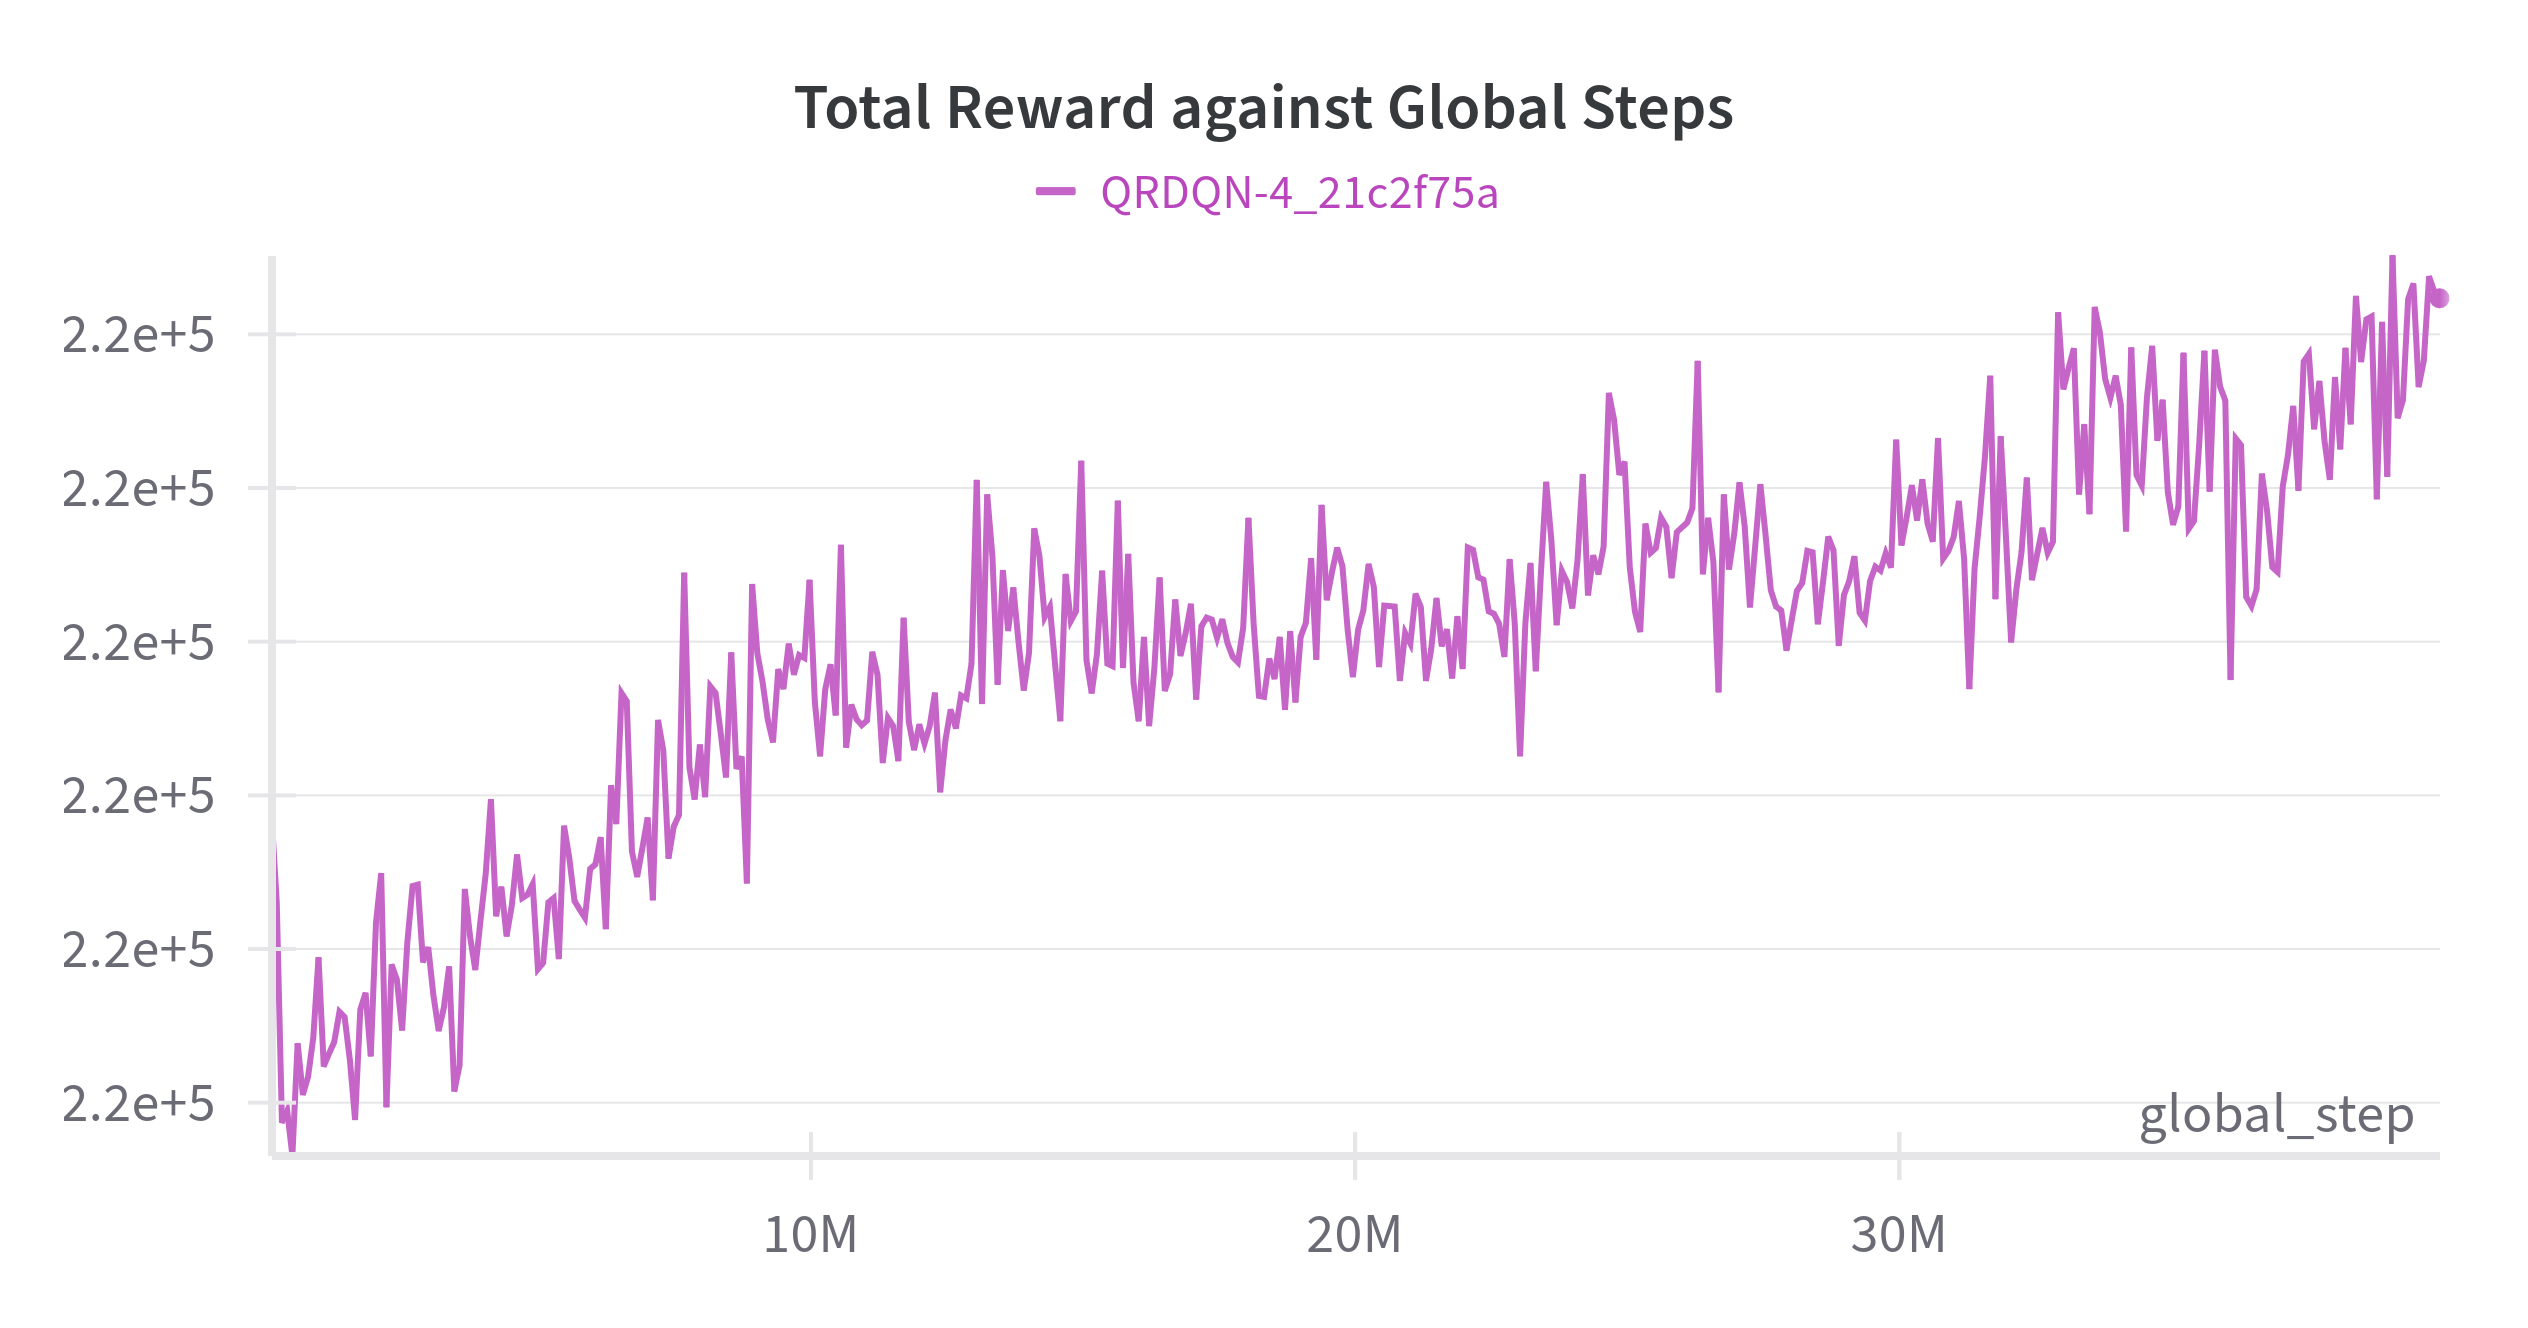
\includegraphics[width=0.49\textwidth]{figures/QRDQN/QRDQN4_Total_Reward.png}}
    \caption{Total Reward of all QRDQN Agents}
    \label{fig:QRDQN_total_reward}
\end{figure}

Compared to the DQN agents, the QR-DQN agents show a more promising performance. Figure \ref{fig:QRDQN_total_reward} shows the performance of all 4 QR-DQN agents of total reward against global steps and shows that all 4 agents had a very similar but consistent growth in performance. It is far more promising than the DQN agents, as the agents were able to increase their total reward consistently throughout training.

Figure \ref{fig:QRDQN_total_reward} (a) shows the performance of QRDQN-1, which shows that the agent had a very consistent growth in performance, but had a sharp fall in performance at the end of training. The sharp fall in performance was just at the end of the 40 million training steps, which is why it is difficult to determine if the agent would have been able to recover from the fall in performance. However, the agent was able to reach a peak performance of 220,490 total reward at around 34 million timesteps. 

Figure \ref{fig:QRDQN_total_reward} (b) shows the performance of QRDQN-2, similarly to QRDQN-1, the agent had a very consistent growth in performance followed by a steep fall in performance towards the end of training. After 28 million timesteps, the agent was able to reach a peak performance of 220,470 total reward. However, at 310 million timesteps, the agent had a sharp fall in performance. After this fall in performance, the agent was never able to recover and reach the same level of performance. Despite the fall in performance, the fall in total reward was only 20, which is insignificant compared to the total reward of 220,470 peak.

Figure \ref{fig:QRDQN_total_reward} (c) shows the performance of QRDQN-3, which had a consistent constant growth in performance throughout training. There were no falls in performance with the exception of a large downwards spike at around 27 million timesteps, which it recovered from. QRDQN-3 had a peak performance of 220,471 total reward at around 34 million timesteps.

Figure \ref{fig:QRDQN_total_reward} (d) shows the performance of QRDQN-4, which again had consistent growth in performance throughout training. The agent had no surprising falls or spikes in growth and had a peak performance of 220,472 total reward at around 38 million timesteps.

\subsubsection*{Loss}

\begin{figure}[H]
    \centering
    \subfigure[QRDQN-1]{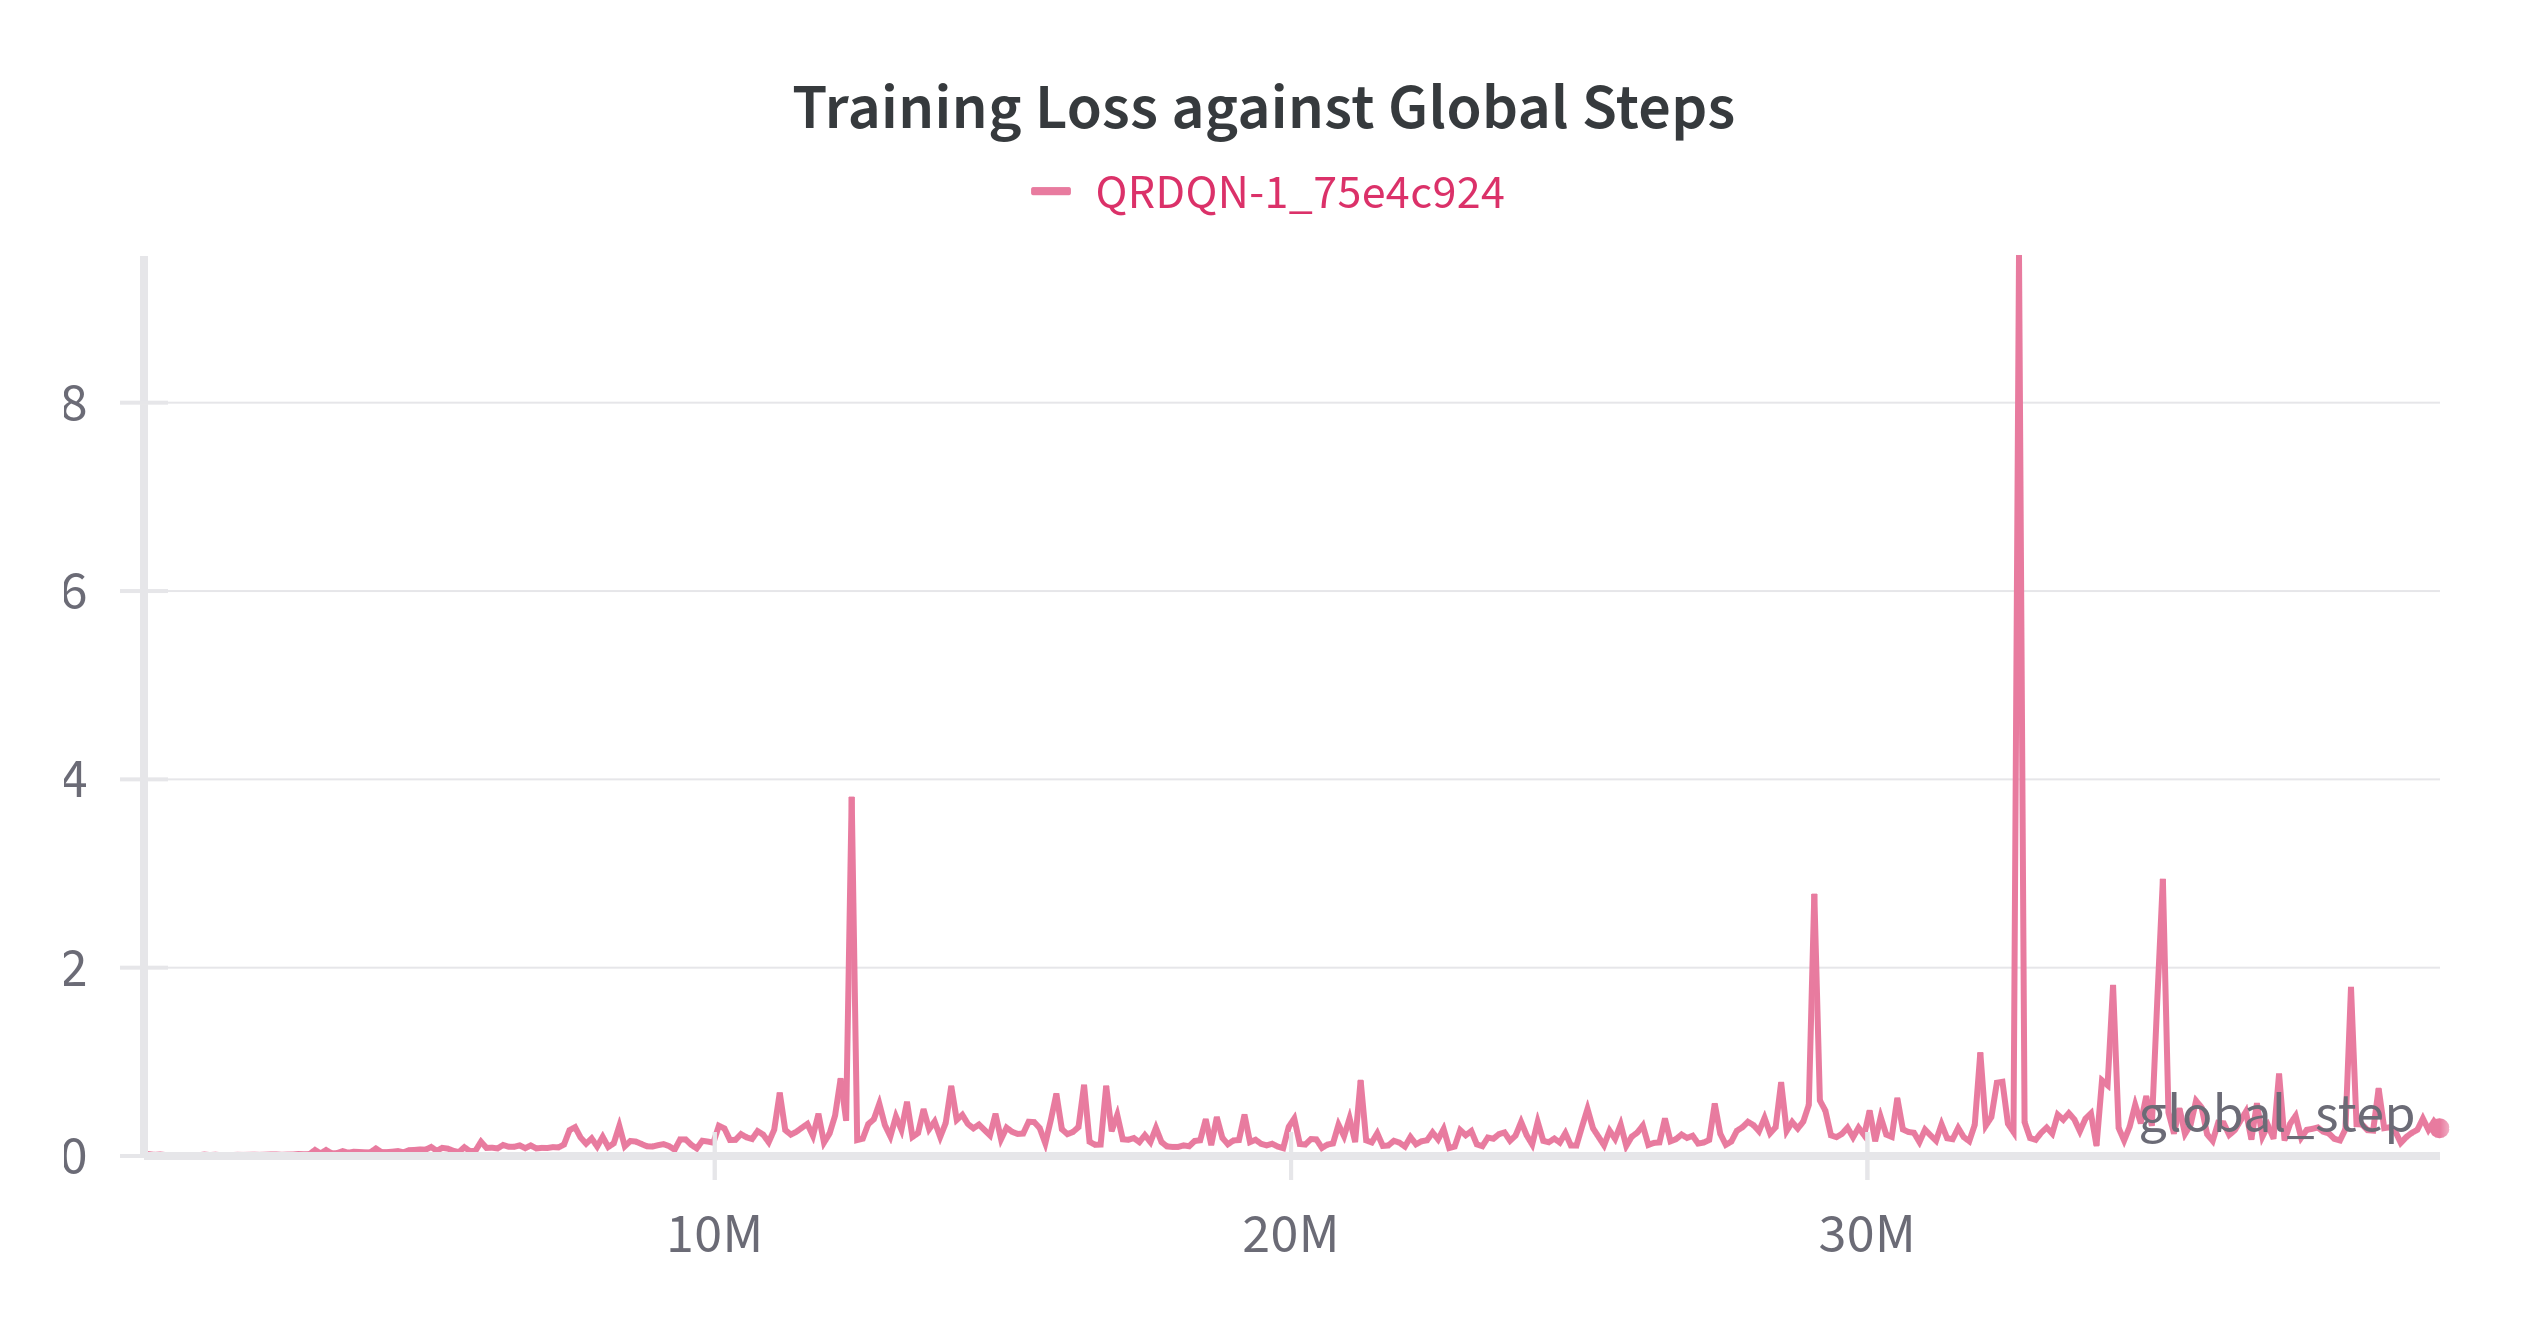
\includegraphics[width=0.49\textwidth]{figures/QRDQN/QRDQN1_Training_Loss.png}} 
    \subfigure[QRDQN-2]{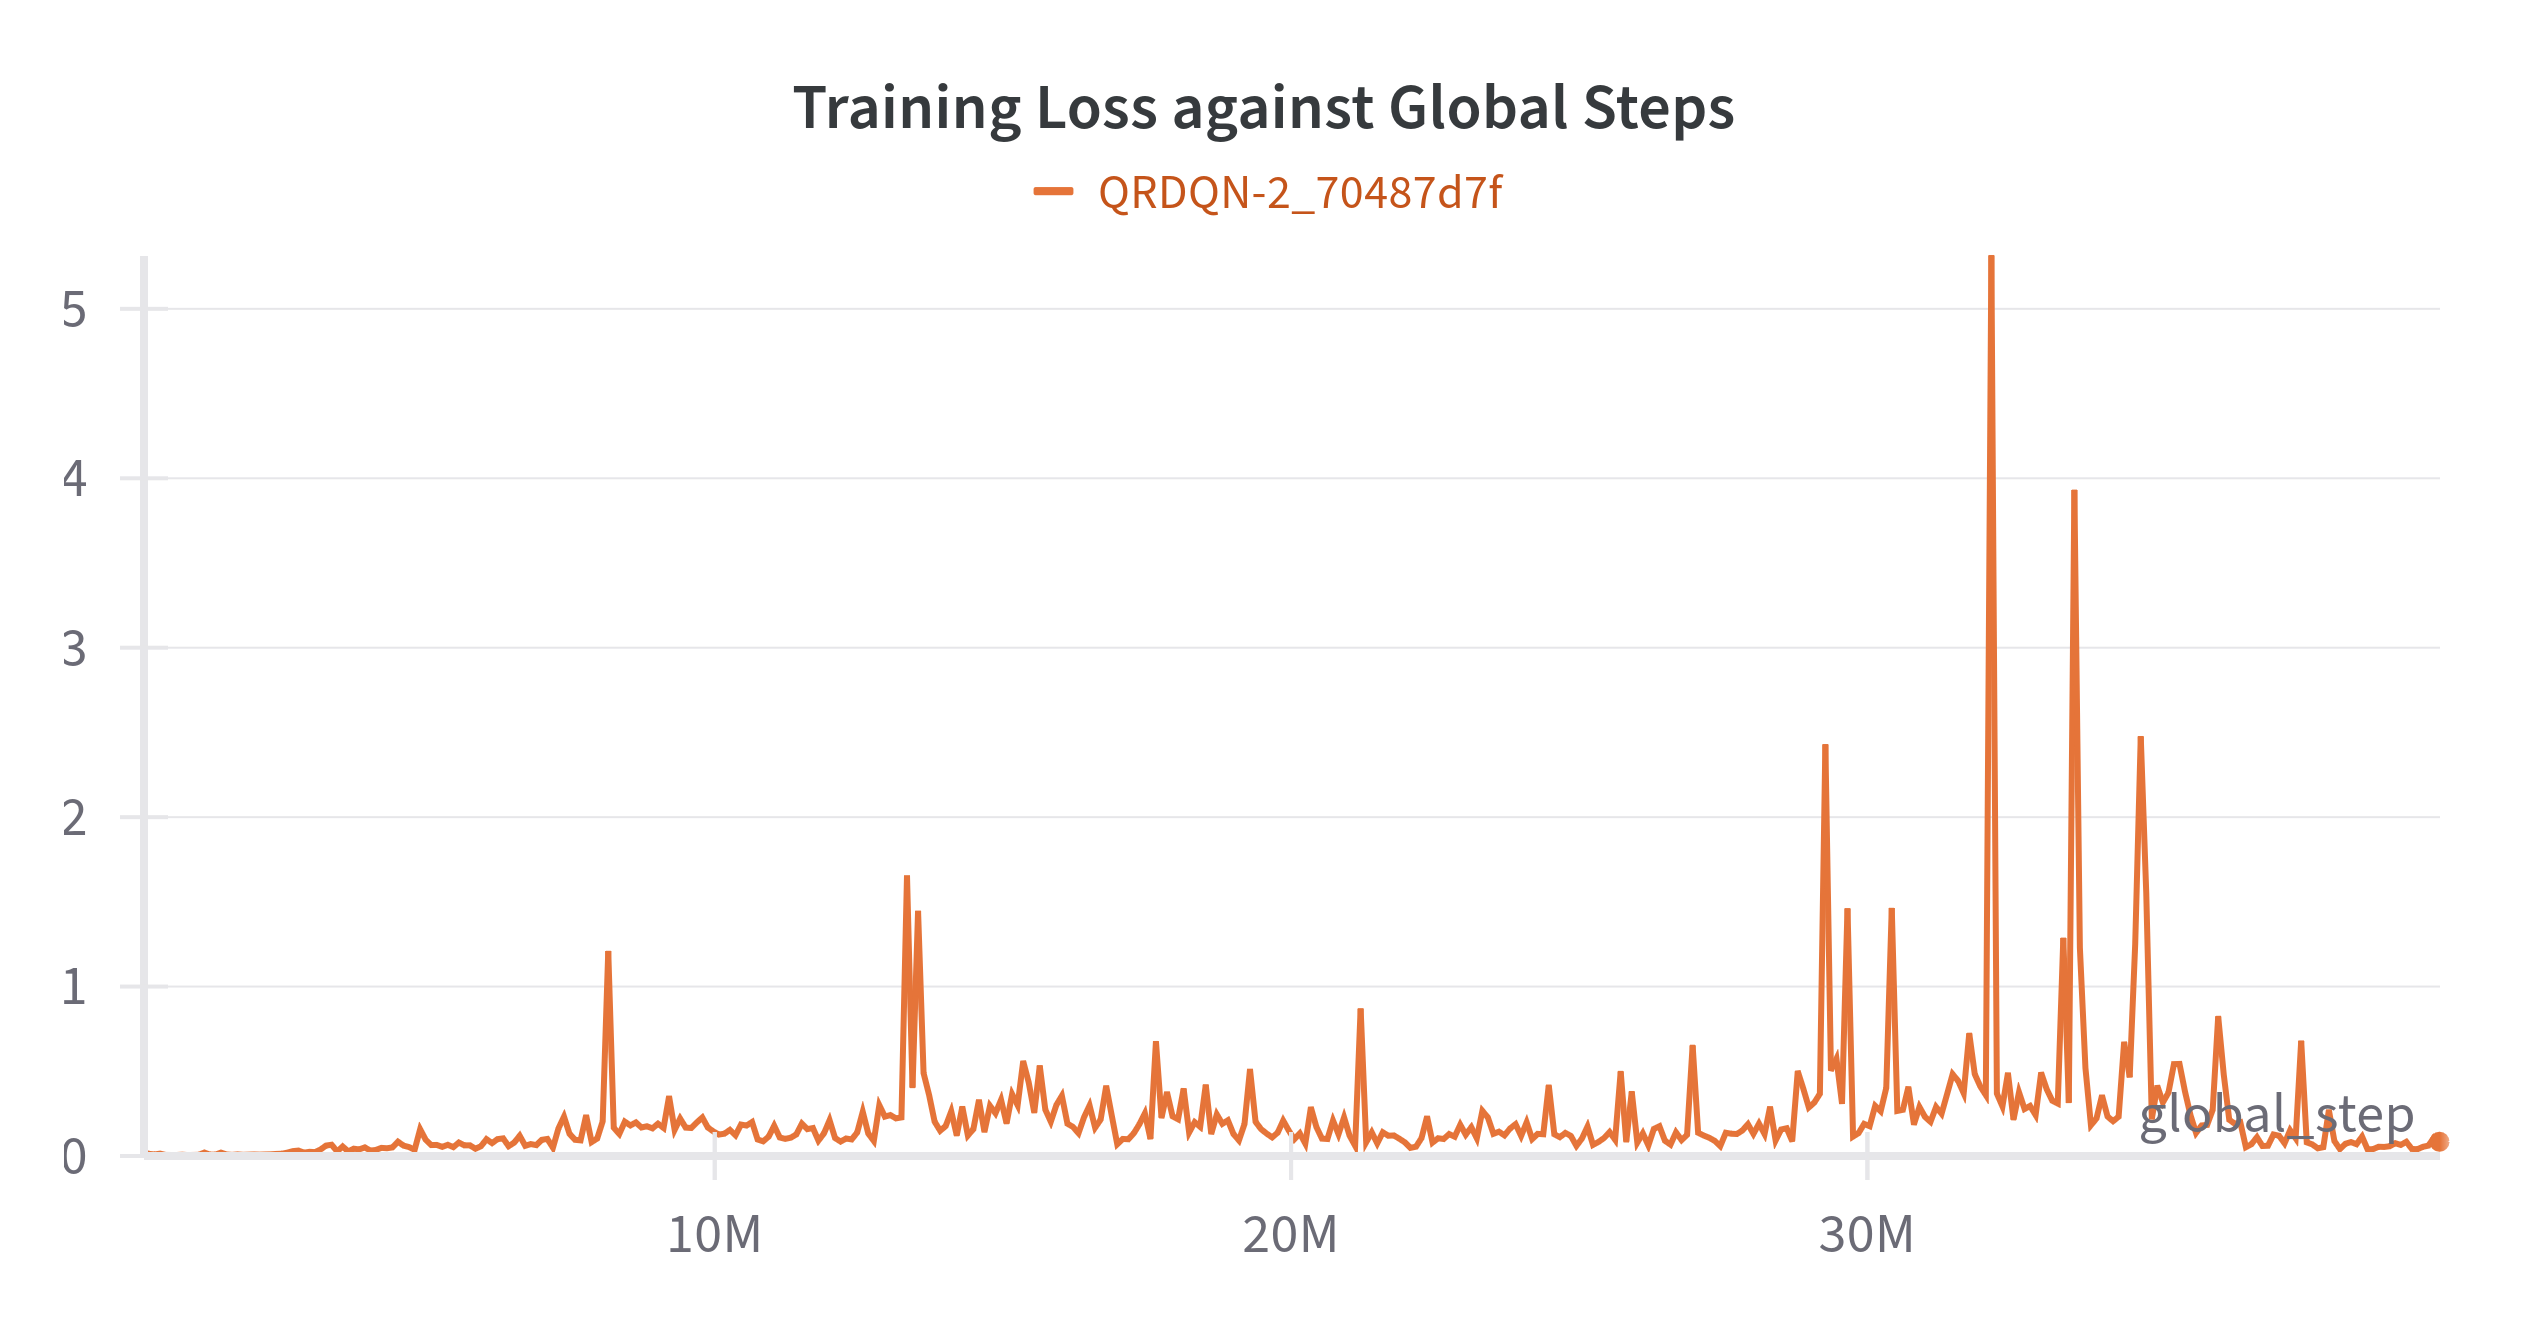
\includegraphics[width=0.49\textwidth]{figures/QRDQN/QRDQN2_Training_Loss.png}} 
    \subfigure[QRDQN-3]{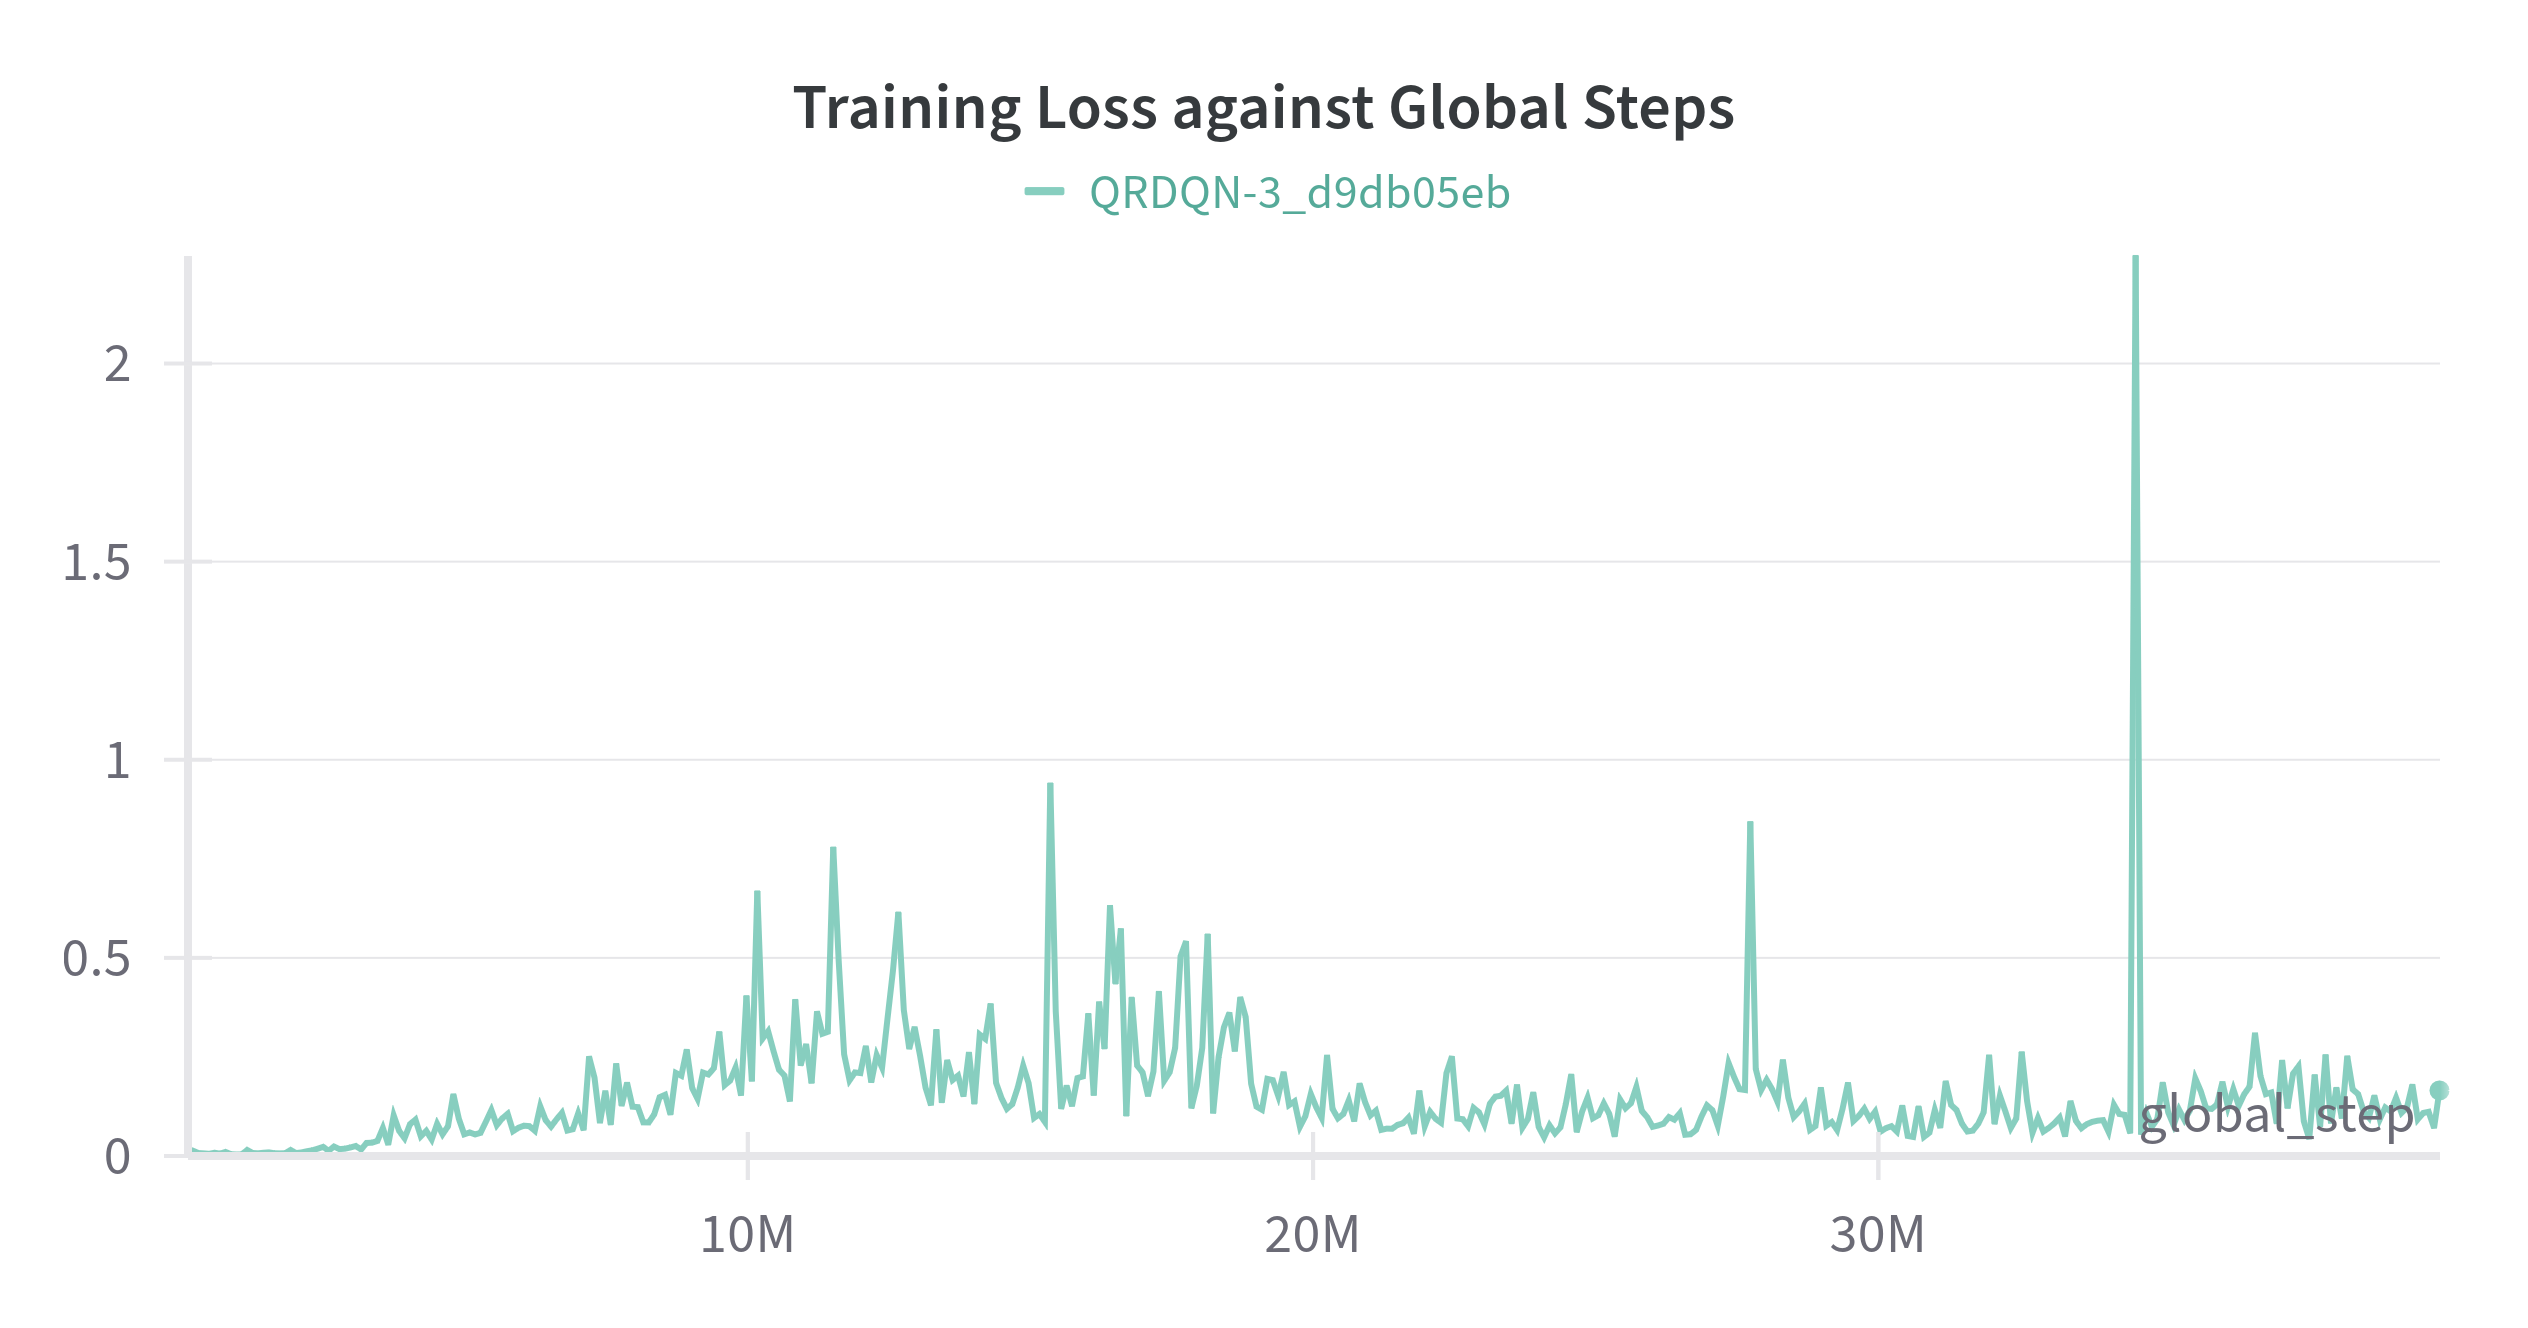
\includegraphics[width=0.49\textwidth]{figures/QRDQN/QRDQN3_Training_Loss.png}}
    \subfigure[QRDQN-4]{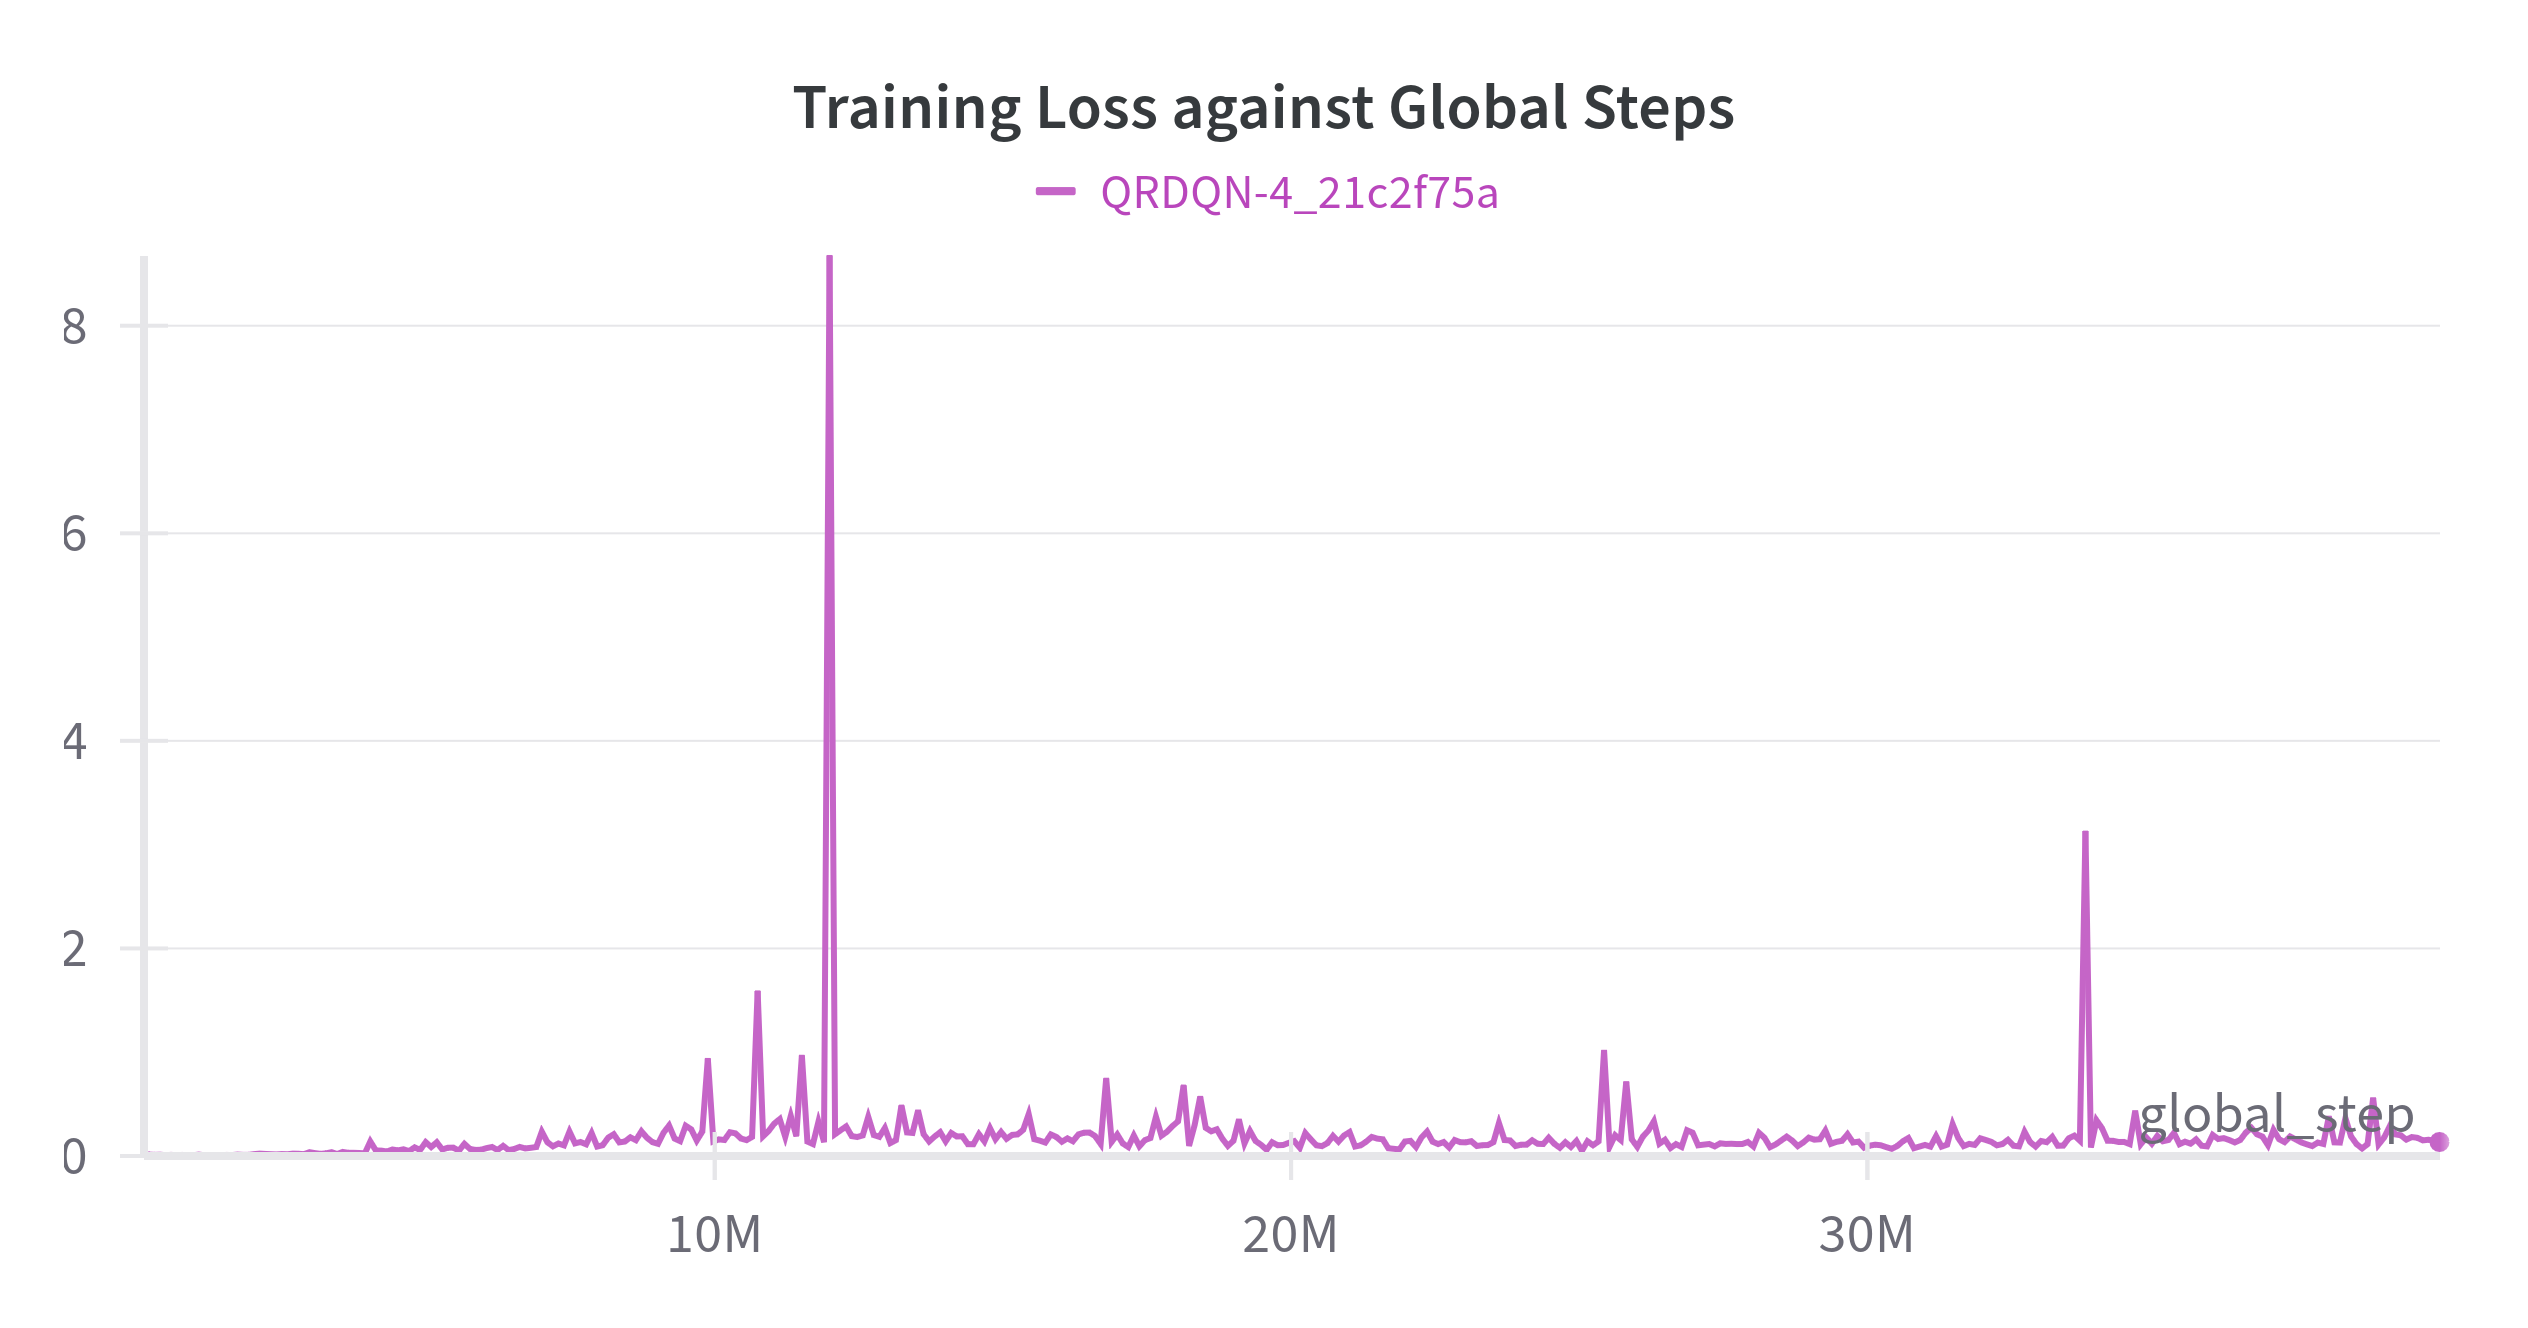
\includegraphics[width=0.49\textwidth]{figures/QRDQN/QRDQN4_Training_Loss.png}}
    \caption{Training Loss of all QRDQN Agents}
    \label{fig:QRDQN_training_loss}
\end{figure}

Figure \ref{fig:QRDQN_training_loss} shows the training loss of each agent shows that all 4 agents showed consistently low loss values with all agents having random spikes throughout training. QRDQN-1 and QRDQN-4 had large spikes of loss values of 8 and above. However, neither of these random spikes were visible on the total reward graphs in figure \ref{fig:QRDQN_total_reward}. Despite QRDQN's better performance compared to DQN, the instability reflected by the relatively higher average loss values compared to DQN suggests that QRDQN's learning process was more inconsistent but better compared to DQN. The interesting thing about QRDQN-3's loss graph is that the agent had an increase in loss value between 10 and 20 million timesteps, which was reflected in its total reward graph by an increase in performance. This suggests that an increase in loss value can both be a sign of unexpectly good or bad performance.

\subsubsection*{Badge Count}

\begin{figure}[H]
    \centering
    \subfigure[QRDQN-1]{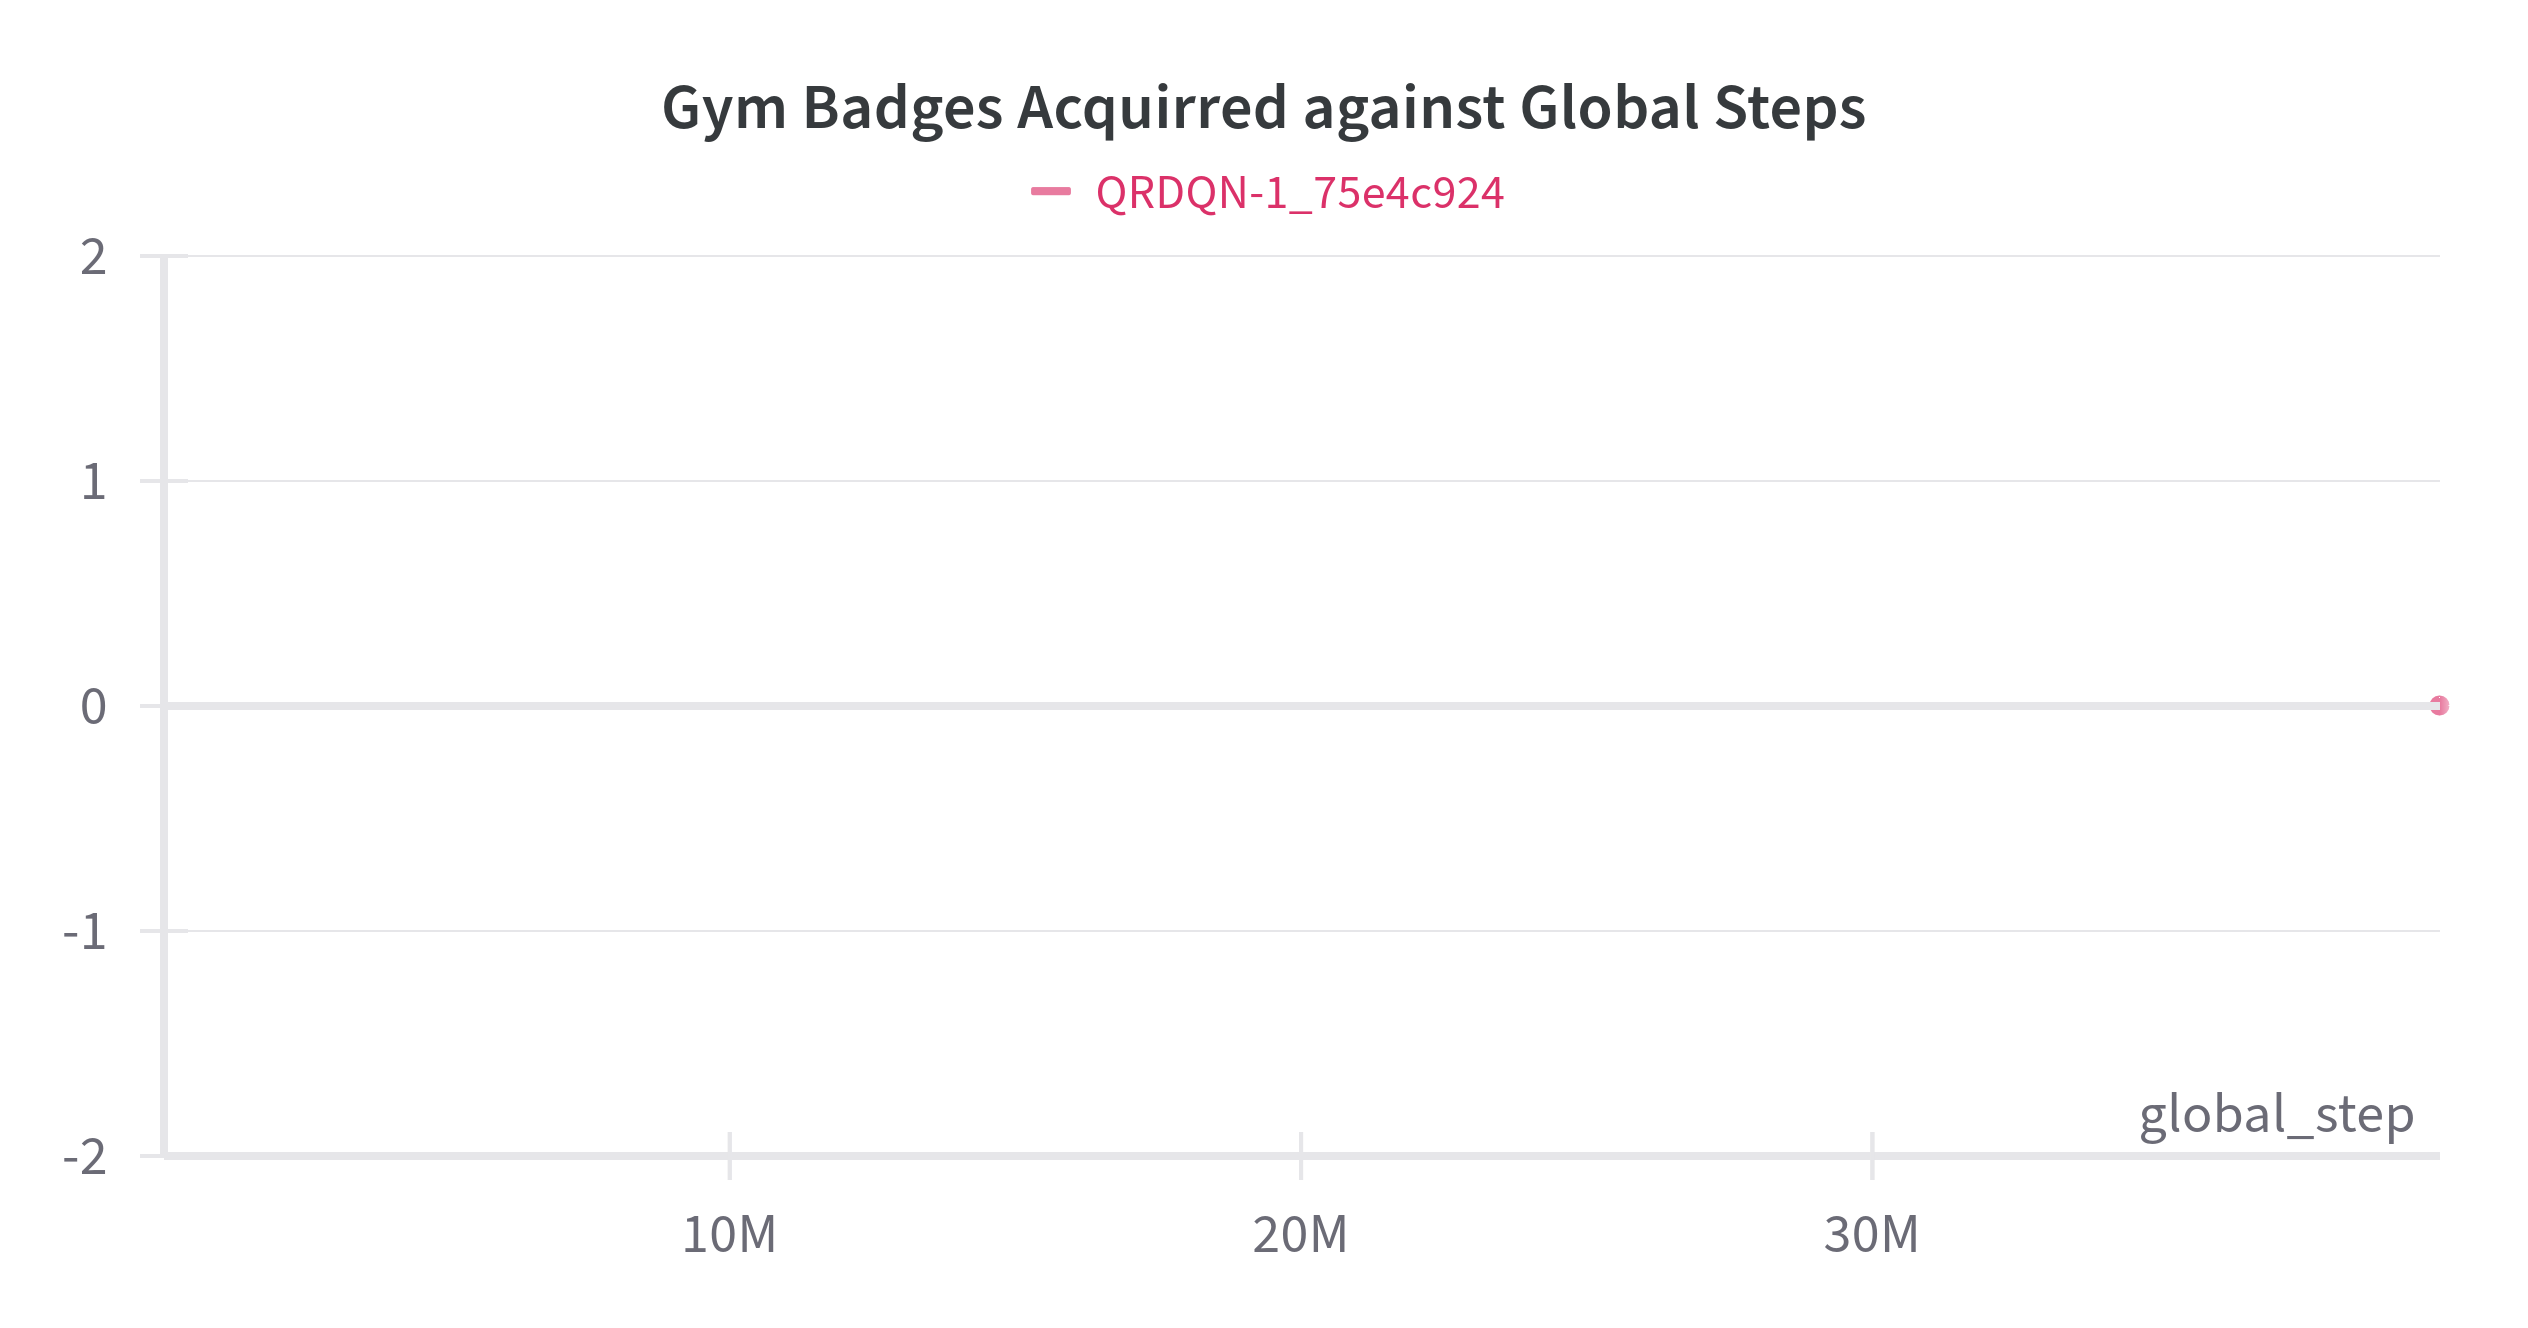
\includegraphics[width=0.49\textwidth]{figures/QRDQN/QRDQN1_Badge_Count.png}} 
    \subfigure[QRDQN-2]{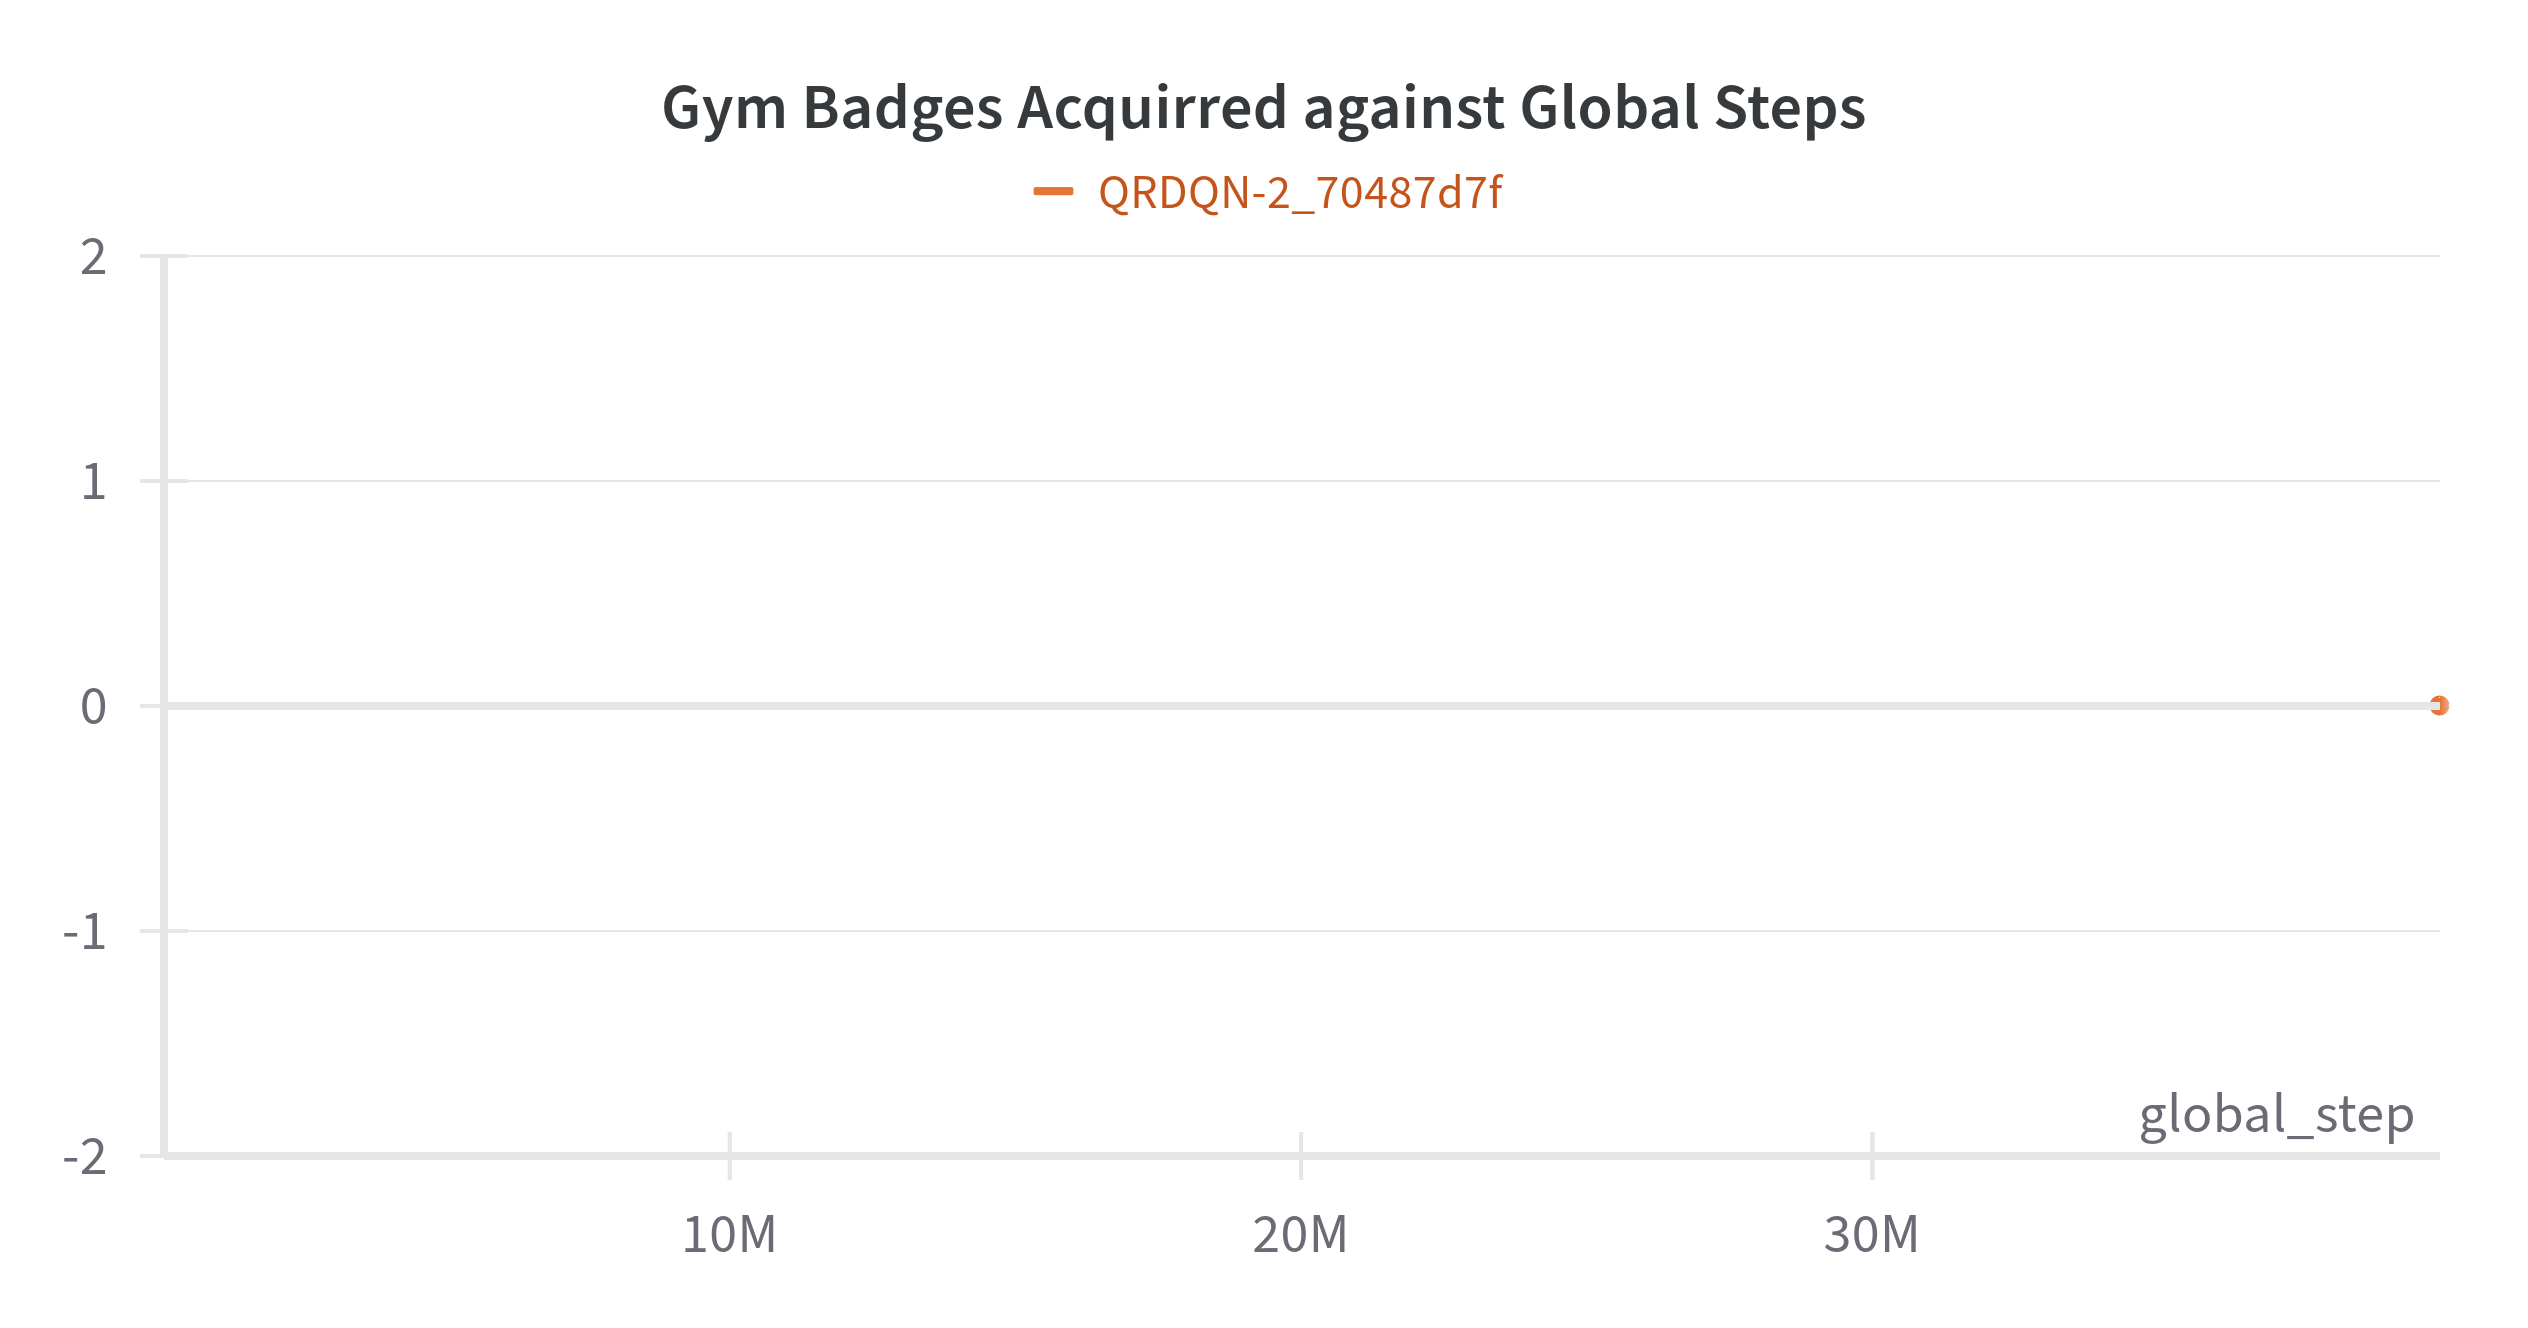
\includegraphics[width=0.49\textwidth]{figures/QRDQN/QRDQN2_Badge_Count.png}} 
    \subfigure[QRDQN-3]{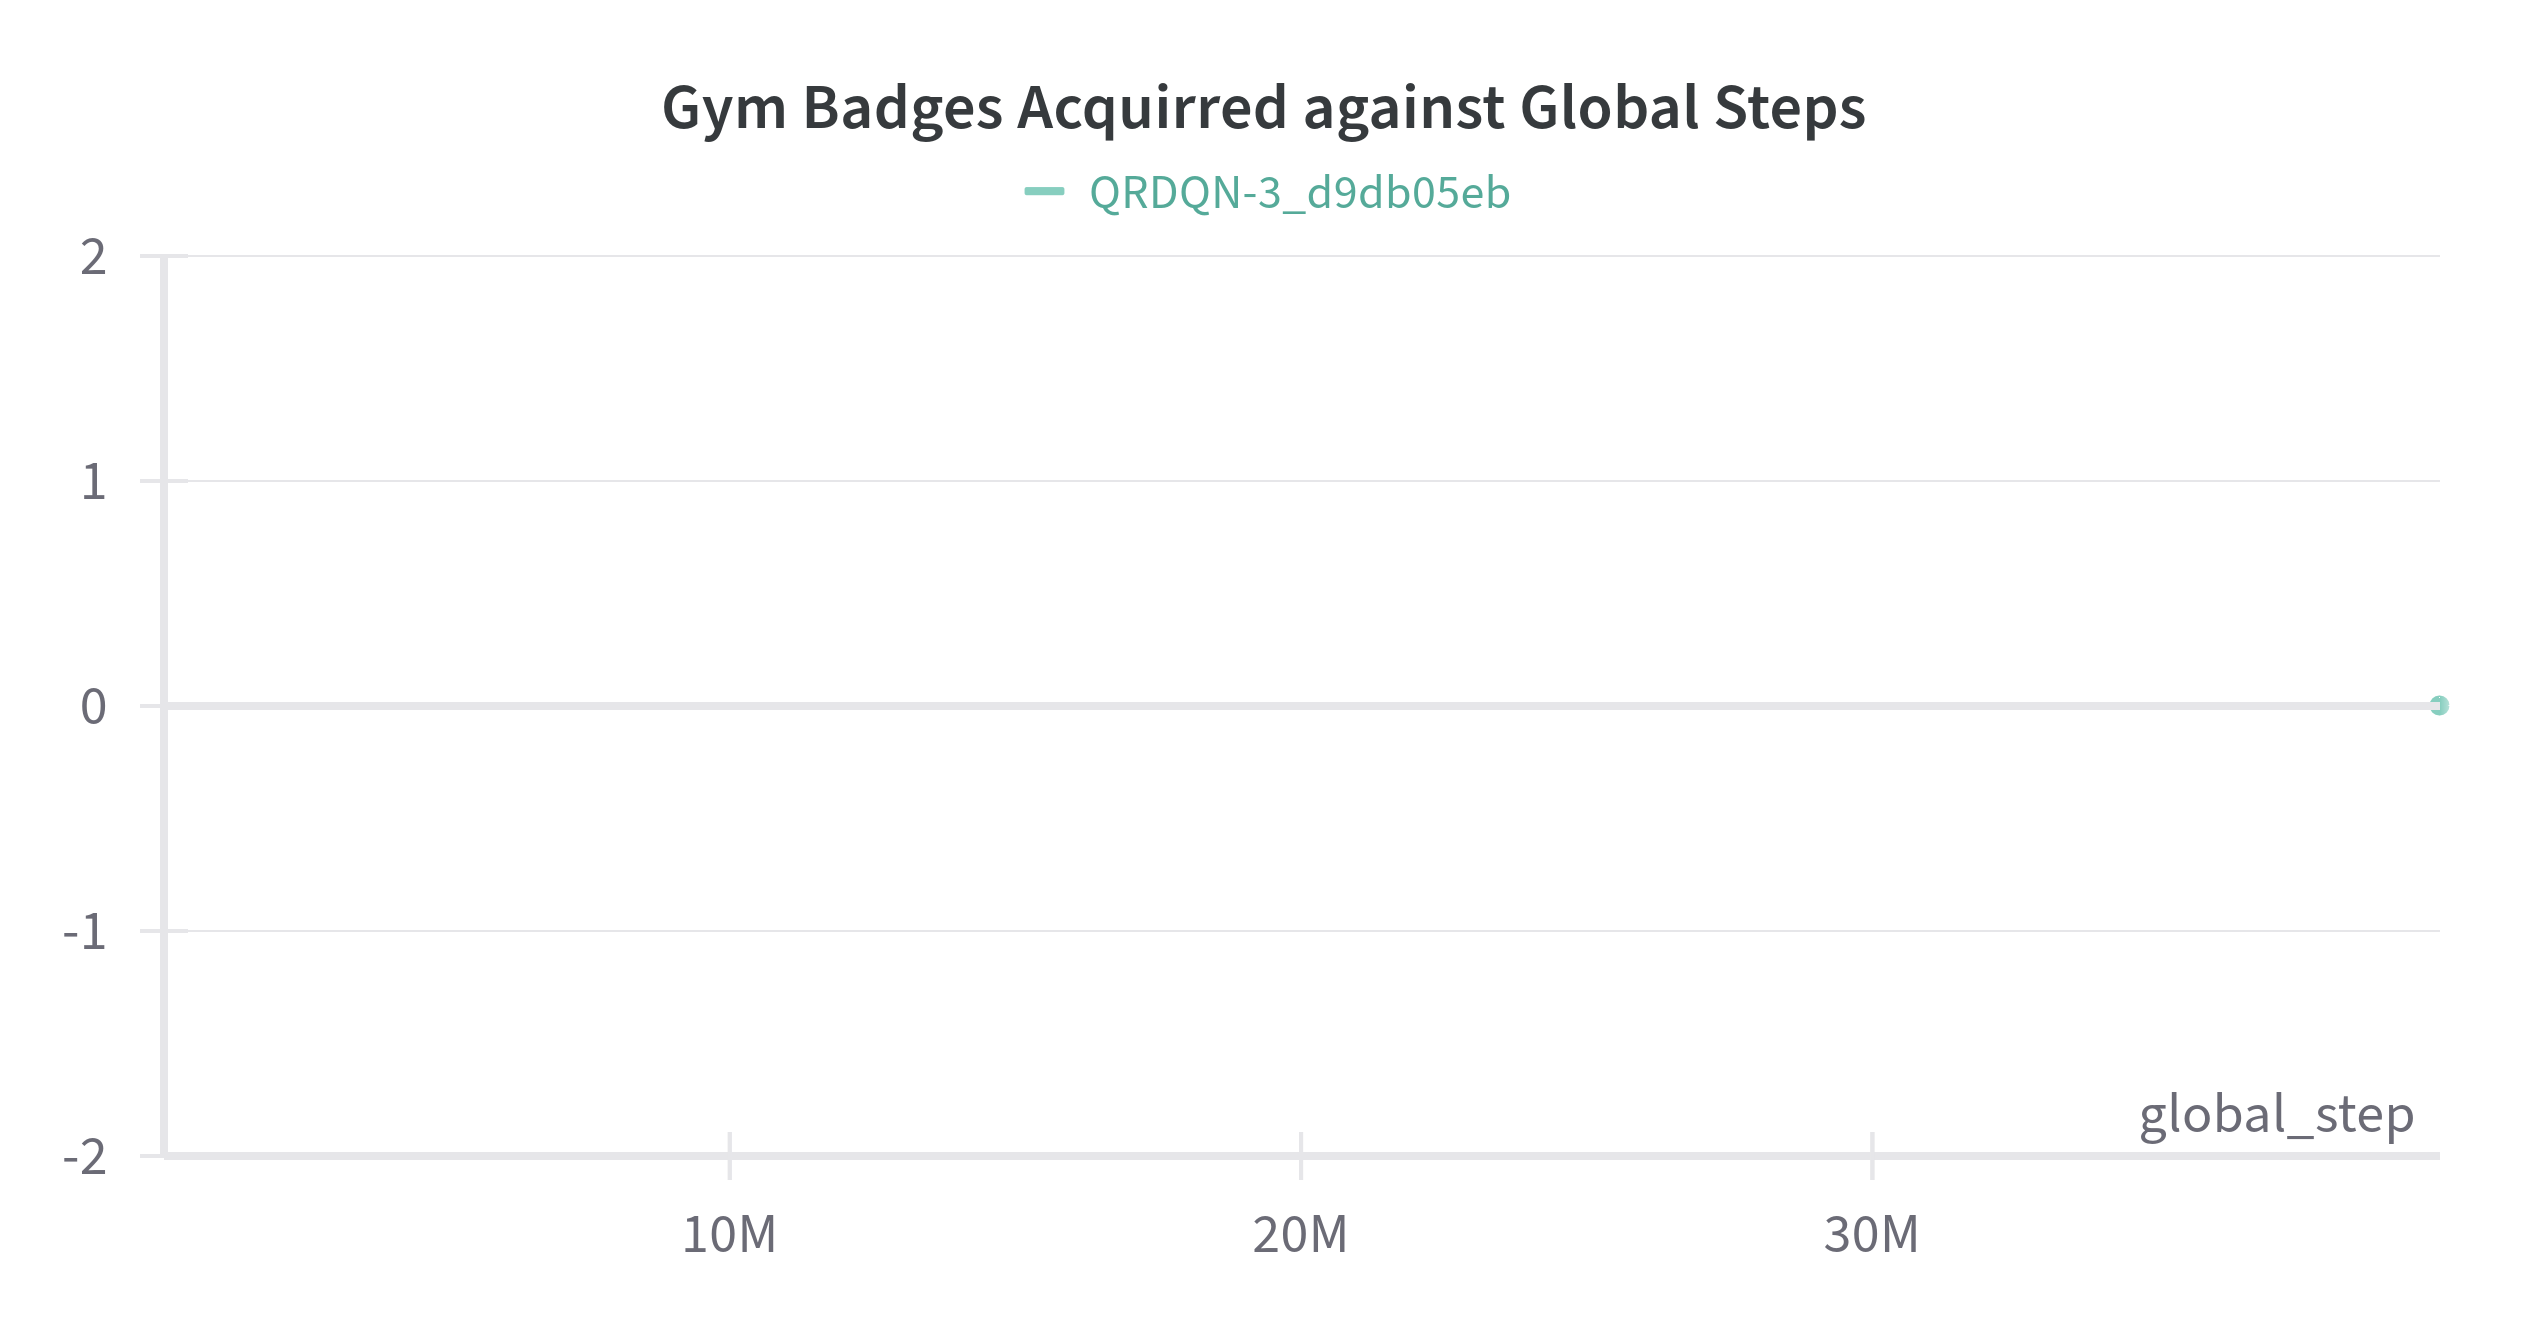
\includegraphics[width=0.49\textwidth]{figures/QRDQN/QRDQN3_Badge_Count.png}} 
    \subfigure[QRDQN-4]{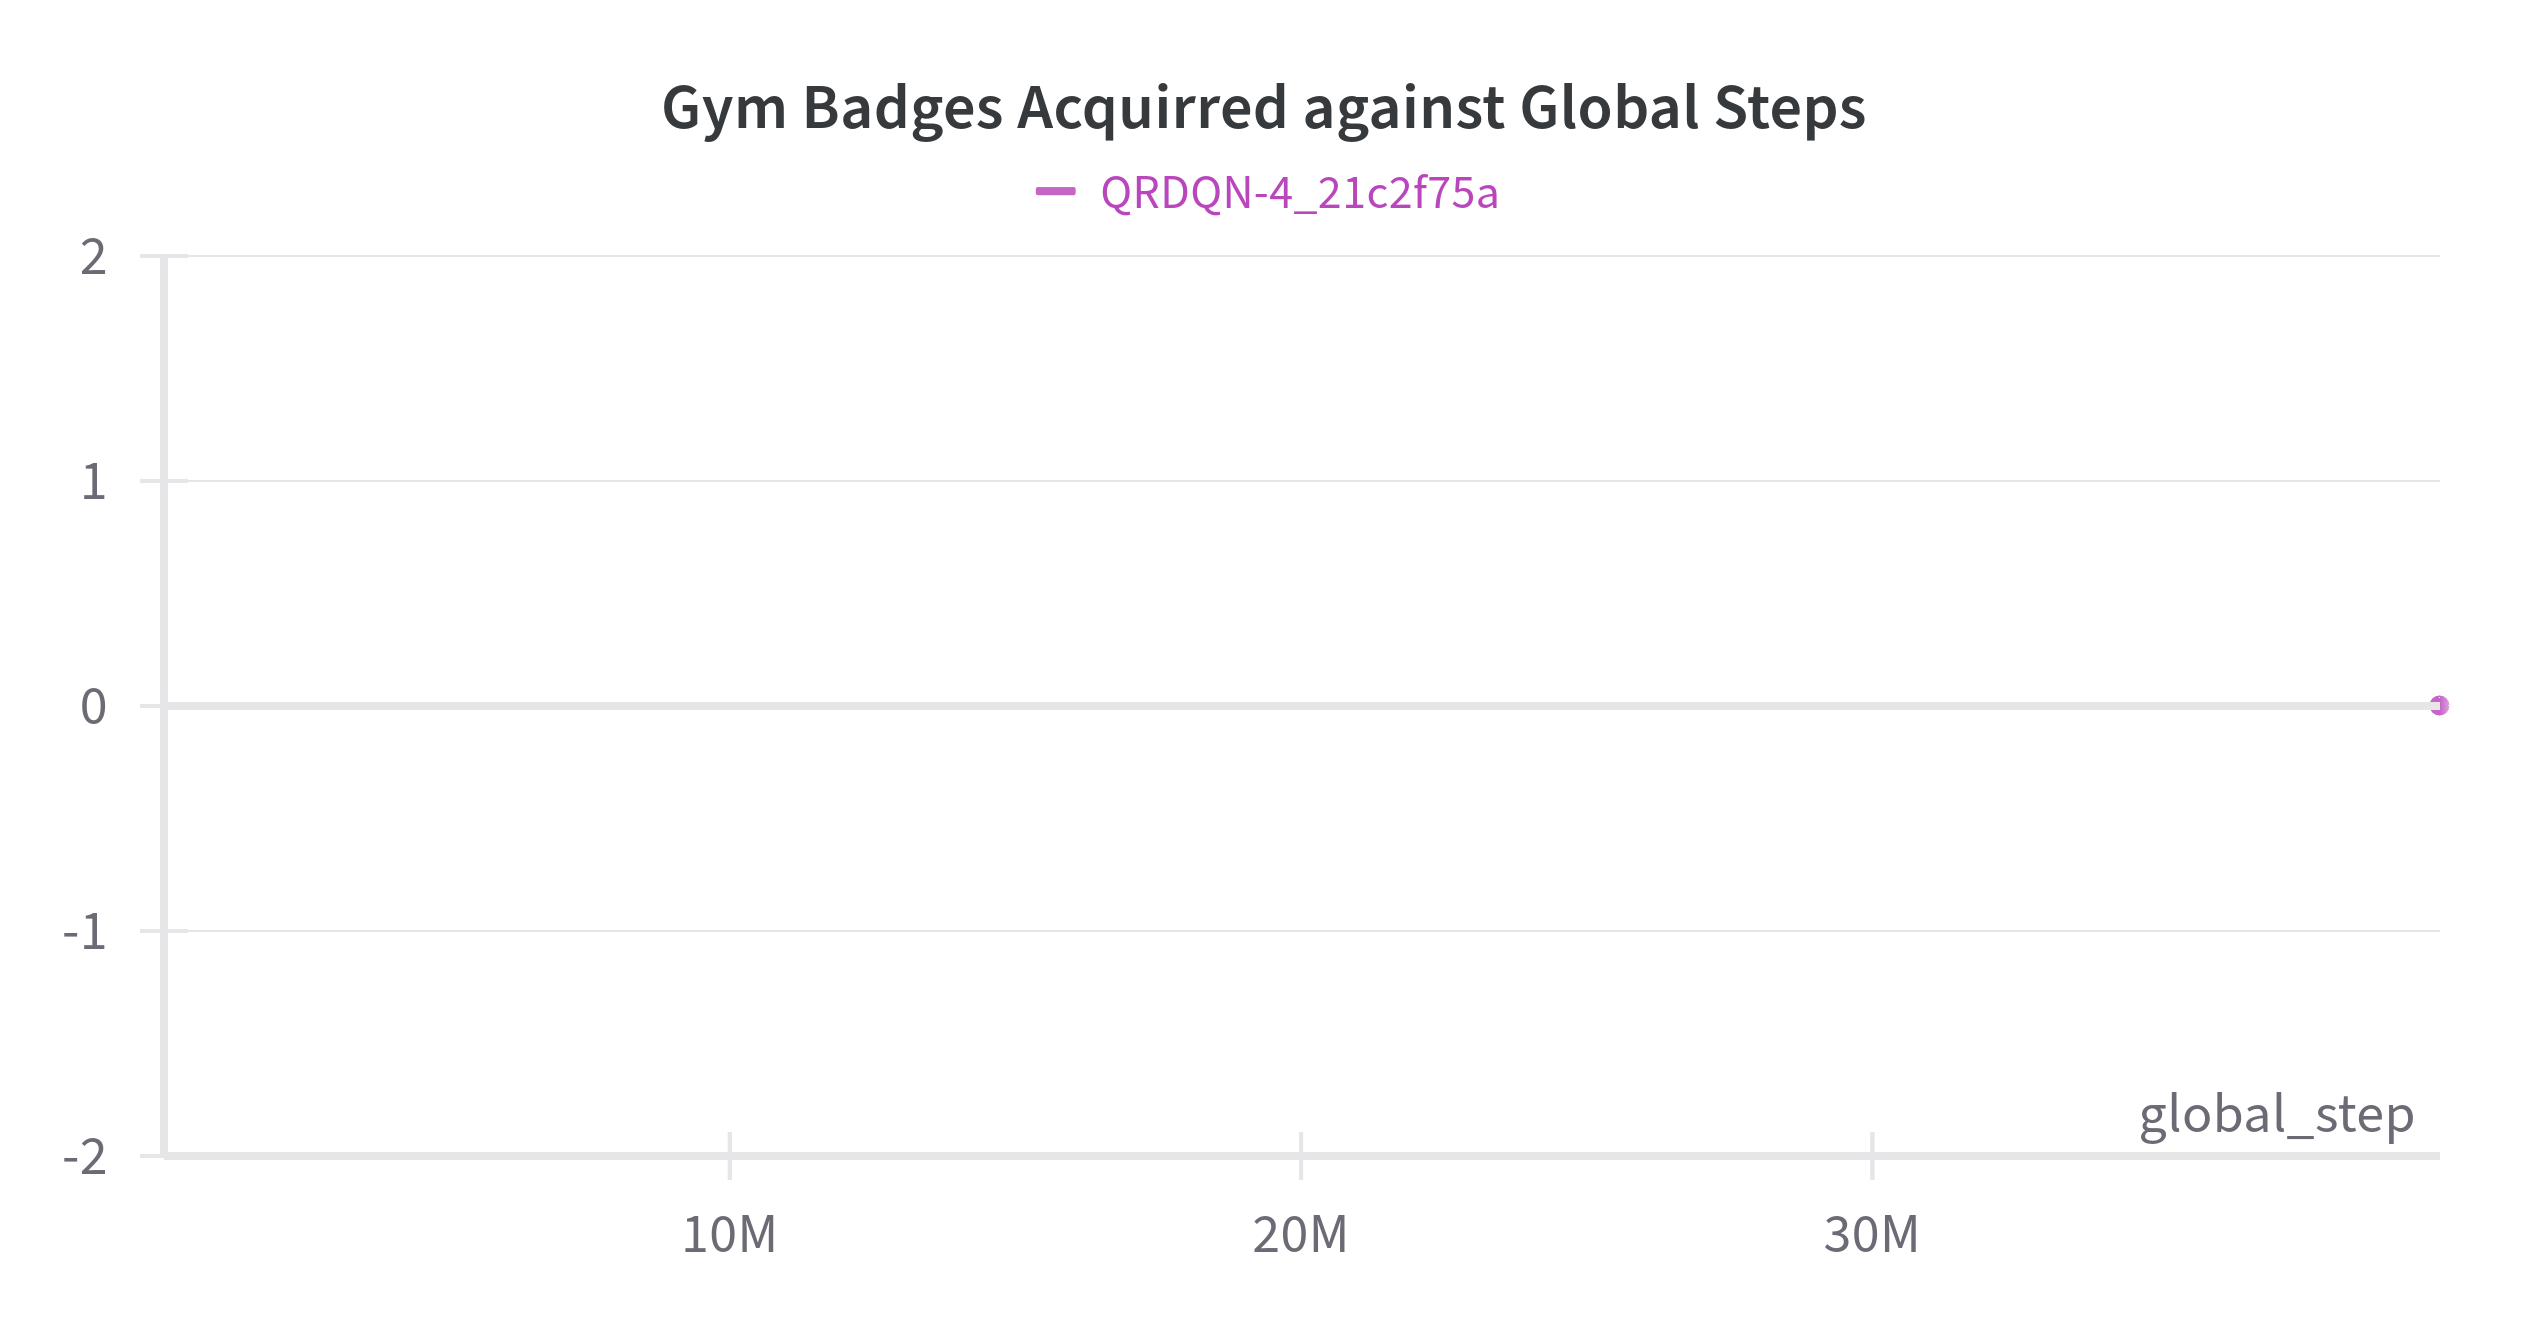
\includegraphics[width=0.49\textwidth]{figures/QRDQN/QRDQN4_Badge_Count.png}} 
    \caption{Badge Count of all QRDQN Agents}
    \label{fig:QRDQN_badge_count}
\end{figure}

Figure \ref{fig:QRDQN_badge_count} shows the badge count of each agent and shows that none of the agents were able to collect the first badge. This suggests that the agents were not able to explore the environment effectively to reach the first gym badge. Despite there being a graduale increase in total reward of each agent throughout training, it was not enough to guide the agent to collect the first badge. 

\subsubsection*{QRDQN Conclusion}

In conclusion, the best performing QRDQN agent from the list of 4 agents is QRDQN-4 because of its both high total reward and lack of any spikes in loss. All 4 QRDQN agents had a consistent growth in performance throughout training, but all other agents had more spikes in loss compared to QRDQN-4. All 4 agents were not able to collect the first gym badge, which further proves that value-based methods are not effective at training agents to explore multi-objective environments. However, the difference between peaks and troughs of total reward suggest that the reward function is not a good guide to completing the objective of the environment.

\subsection{PPO}

\begin{center}
    \begin{tabular}{ |c|c| } 
     \hline
     Hyperparameter & Value \\ 
     \hline
     Total Timesteps & 40,05,000 \\
     Number of Episodes &  1,905 \\
     Episode Length & 1,500 \\ 
     Parallel Instances & 14 \\
     Policy Model & MultiInputPolicy \\
     Gamma & 0.99 \\  
     Batch Size & 64 \\
     \hline
    \end{tabular}
    \end{center}

The training script used to train all 4 agents can be found within the research paper's GitHub repository under ``run\_baseline\_PPO.py''. A total of 14 parallel instances of the environment was trained at the same time to train for 1,905 episodes total, where each episode is 1,500 steps long. This totals up to 40,005,000 steps in total. The performance of the 4 agents can be seen on figure \ref{fig:PPO_total_reward}. 

\subsubsection*{Total Reward}

\begin{figure}[H]
    \centering
    \subfigure[PPO-1]{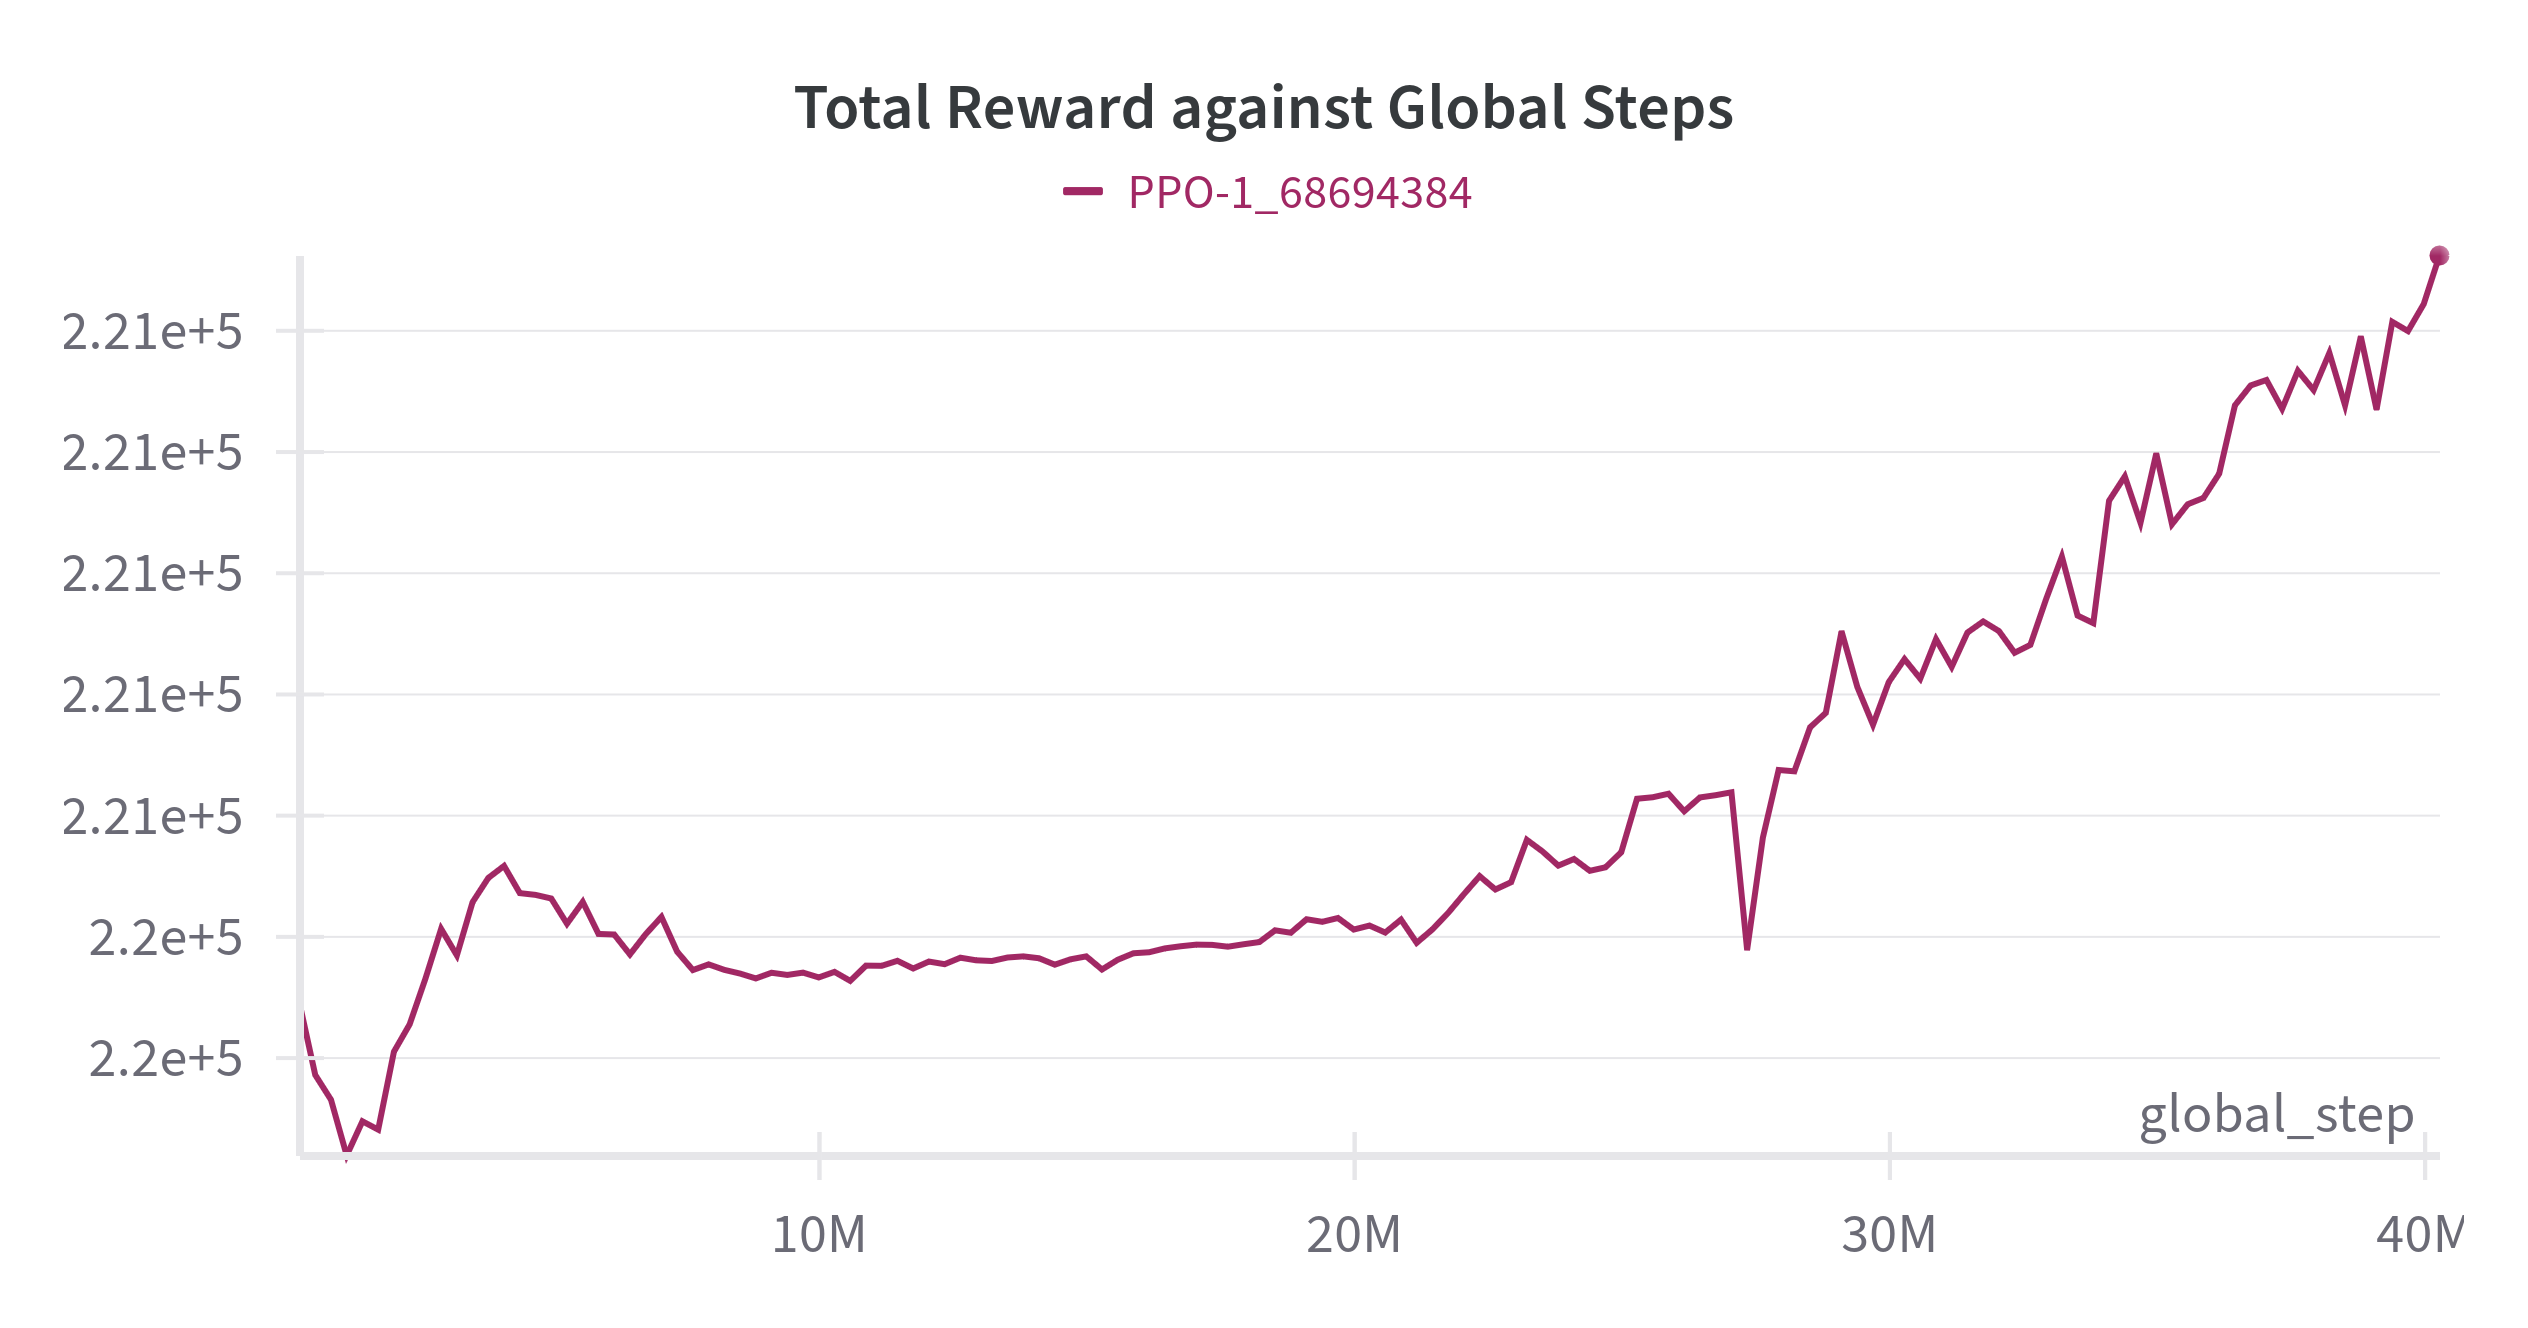
\includegraphics[width=0.49\textwidth]{figures/PPO/PPO1_Total_Reward.png}} 
    \subfigure[PPO-2]{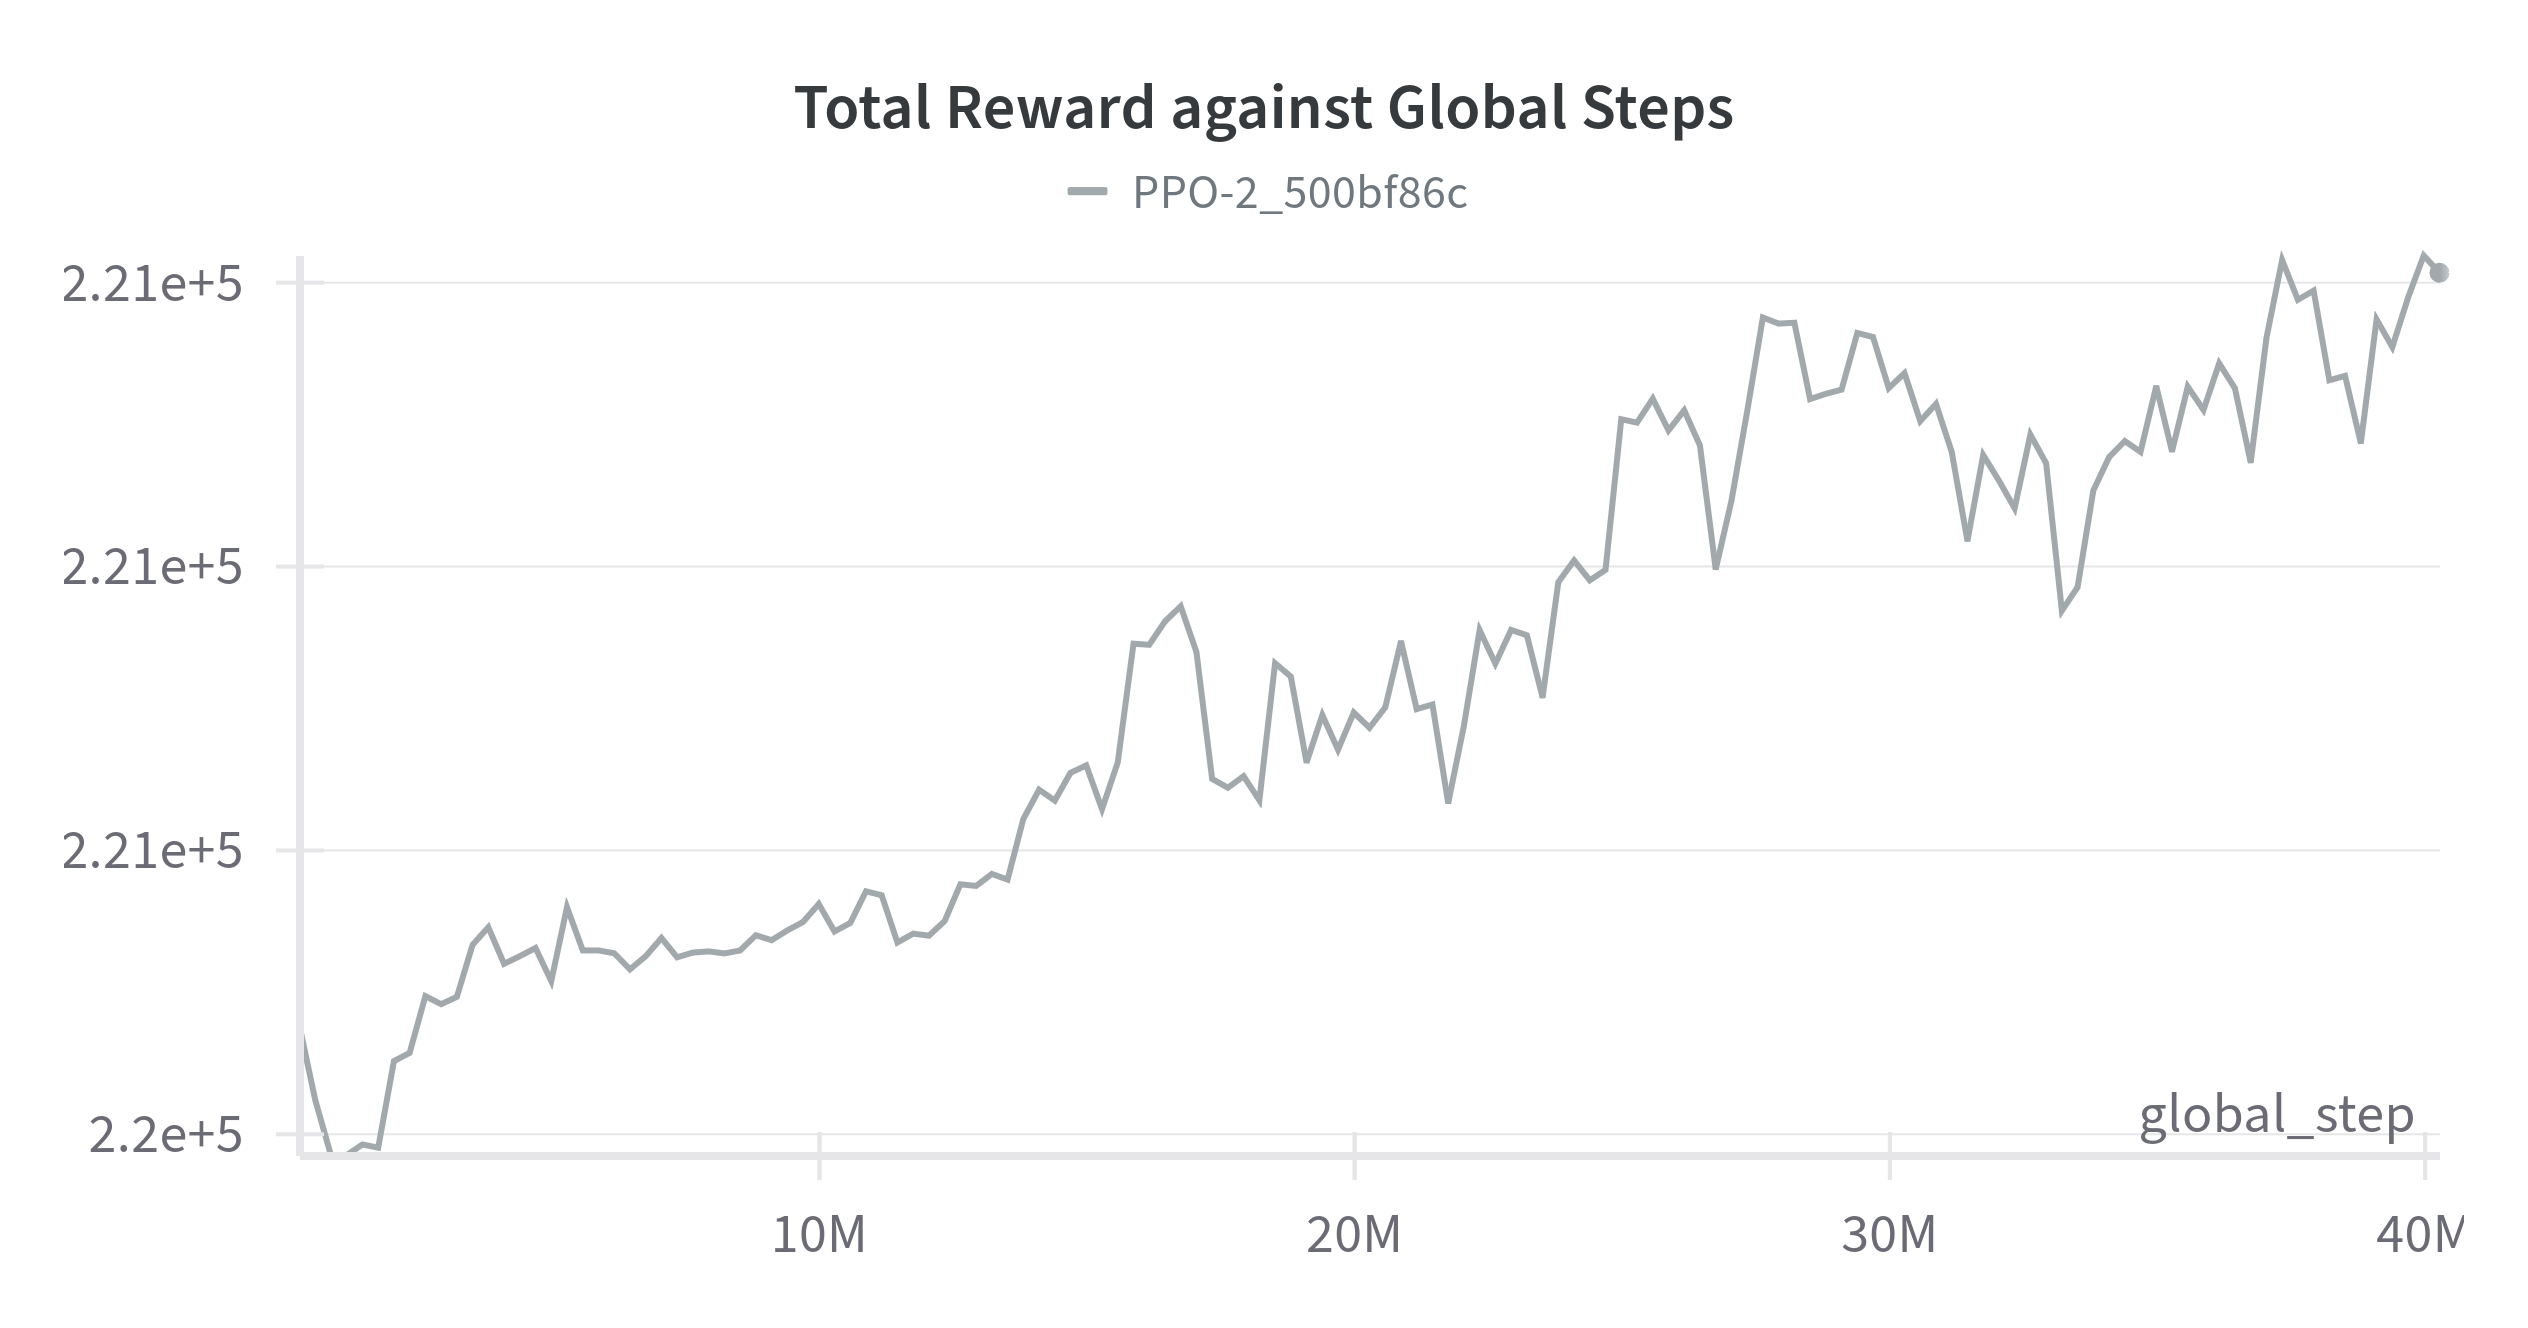
\includegraphics[width=0.49\textwidth]{figures/PPO/PPO2_Total_Reward.png}} 
    \subfigure[PPO-3]{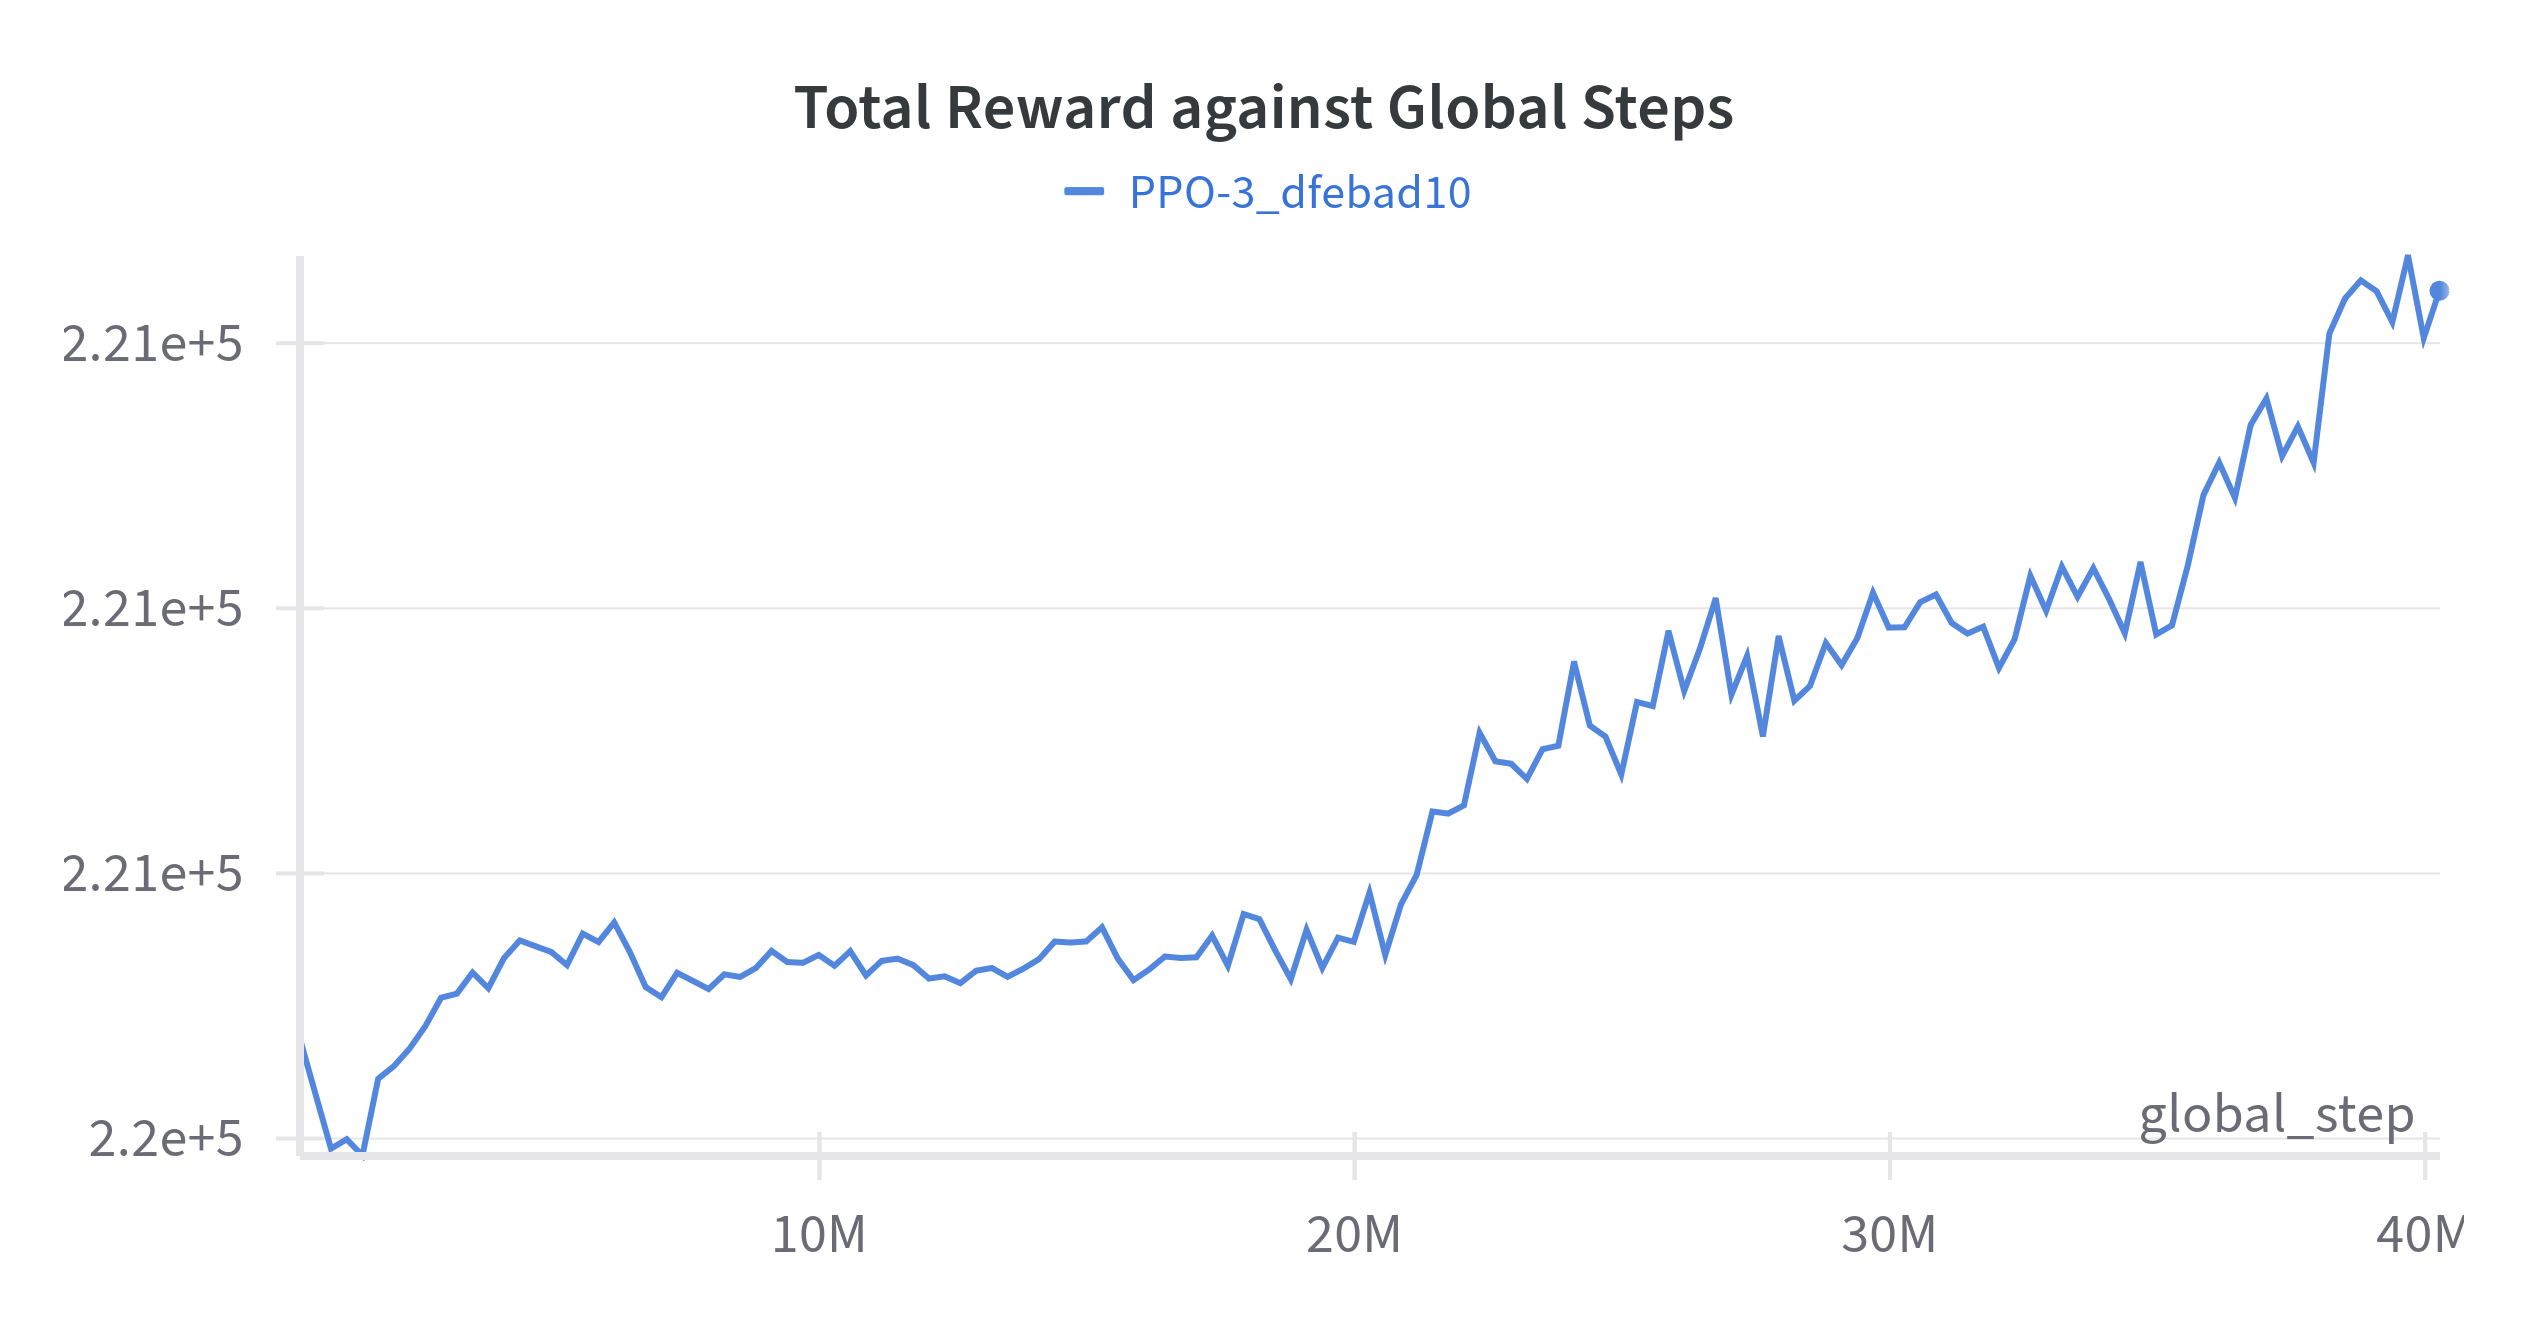
\includegraphics[width=0.49\textwidth]{figures/PPO/PPO3_Total_Reward.png}}
    \subfigure[PPO-4]{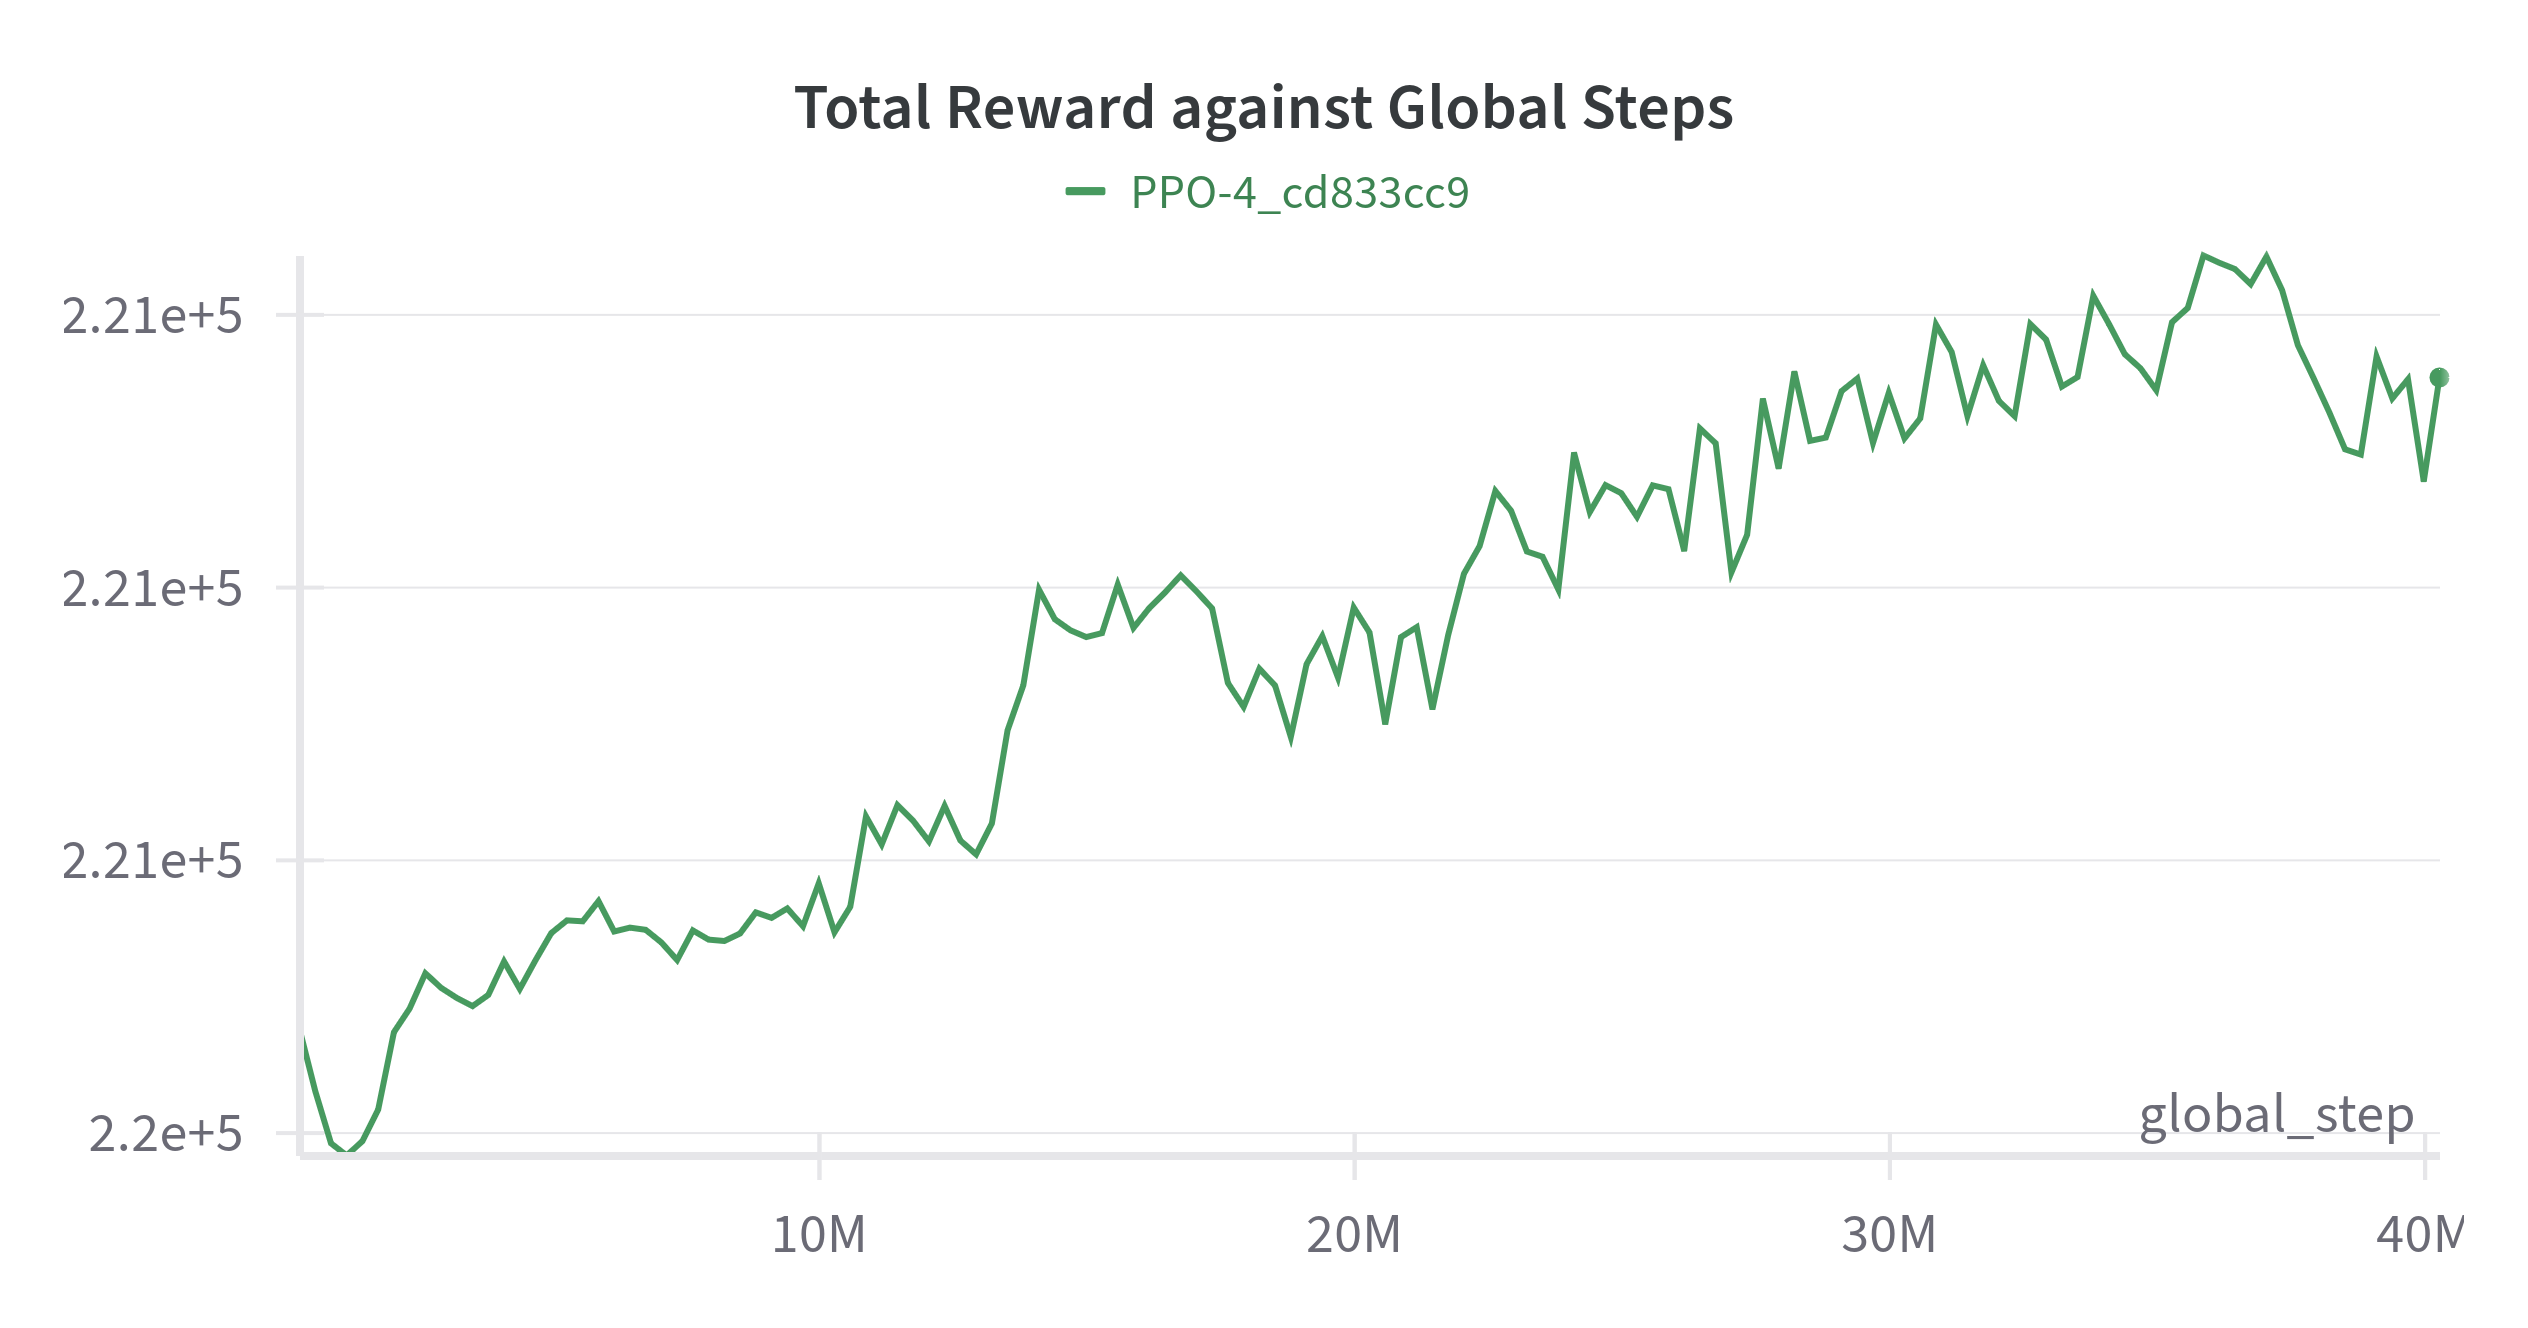
\includegraphics[width=0.49\textwidth]{figures/PPO/PPO4_Total_Reward.png}}
    \caption{Total Reward of all PPO Agents}
    \label{fig:PPO_total_reward}
\end{figure}

Looking at the performance of all 4 PPO agents, all the agents showed very strong signs of learning the environment and reaching the optimal policy. All agents started off with a steep growth in total reward before maintained a gradual growth throughout training and all agents did not have any drops or sharp falls in total reward. Deciding the best performing agent among the 4 is difficult because all agents have very similar positive trajectories in performance. 

Figure \ref{fig:PPO_total_reward} (a) shows the performance of PPO-1, which shows steady growth through out the first 26 million timesteps, before experincing a sudden drop in total reward before recovering and growing again to a peak of 220529 total reward at 40 million timesteps.

Figure \ref{fig:PPO_total_reward} (b) shows the performance of PPO-2, which shows steady but inconsistent growth throughout the training. The agent was able to consistently improve its total reward throughout training, but experienced many random positive and negative spikes in performance.

Figure \ref{fig:PPO_total_reward} (c) shows the performance of PPO-3, which had visibly the slowest growth in performance compared to the other agents. However, was still able to achieve the highest reward of 220,616 total reward at 40 million timesteps.

Figure \ref{fig:PPO_total_reward} (d) shows the performance of PPO-4, which shows a very straight growth in performance throughout training. The consistency of the growth is so consistent a straight line can be drawn through the graph. The agent was able to reach a peak of 220,610 total reward at 35 million timesteps.

\subsubsection*{Loss}
\begin{figure}[H]
    \centering
    \subfigure[PPO-1]{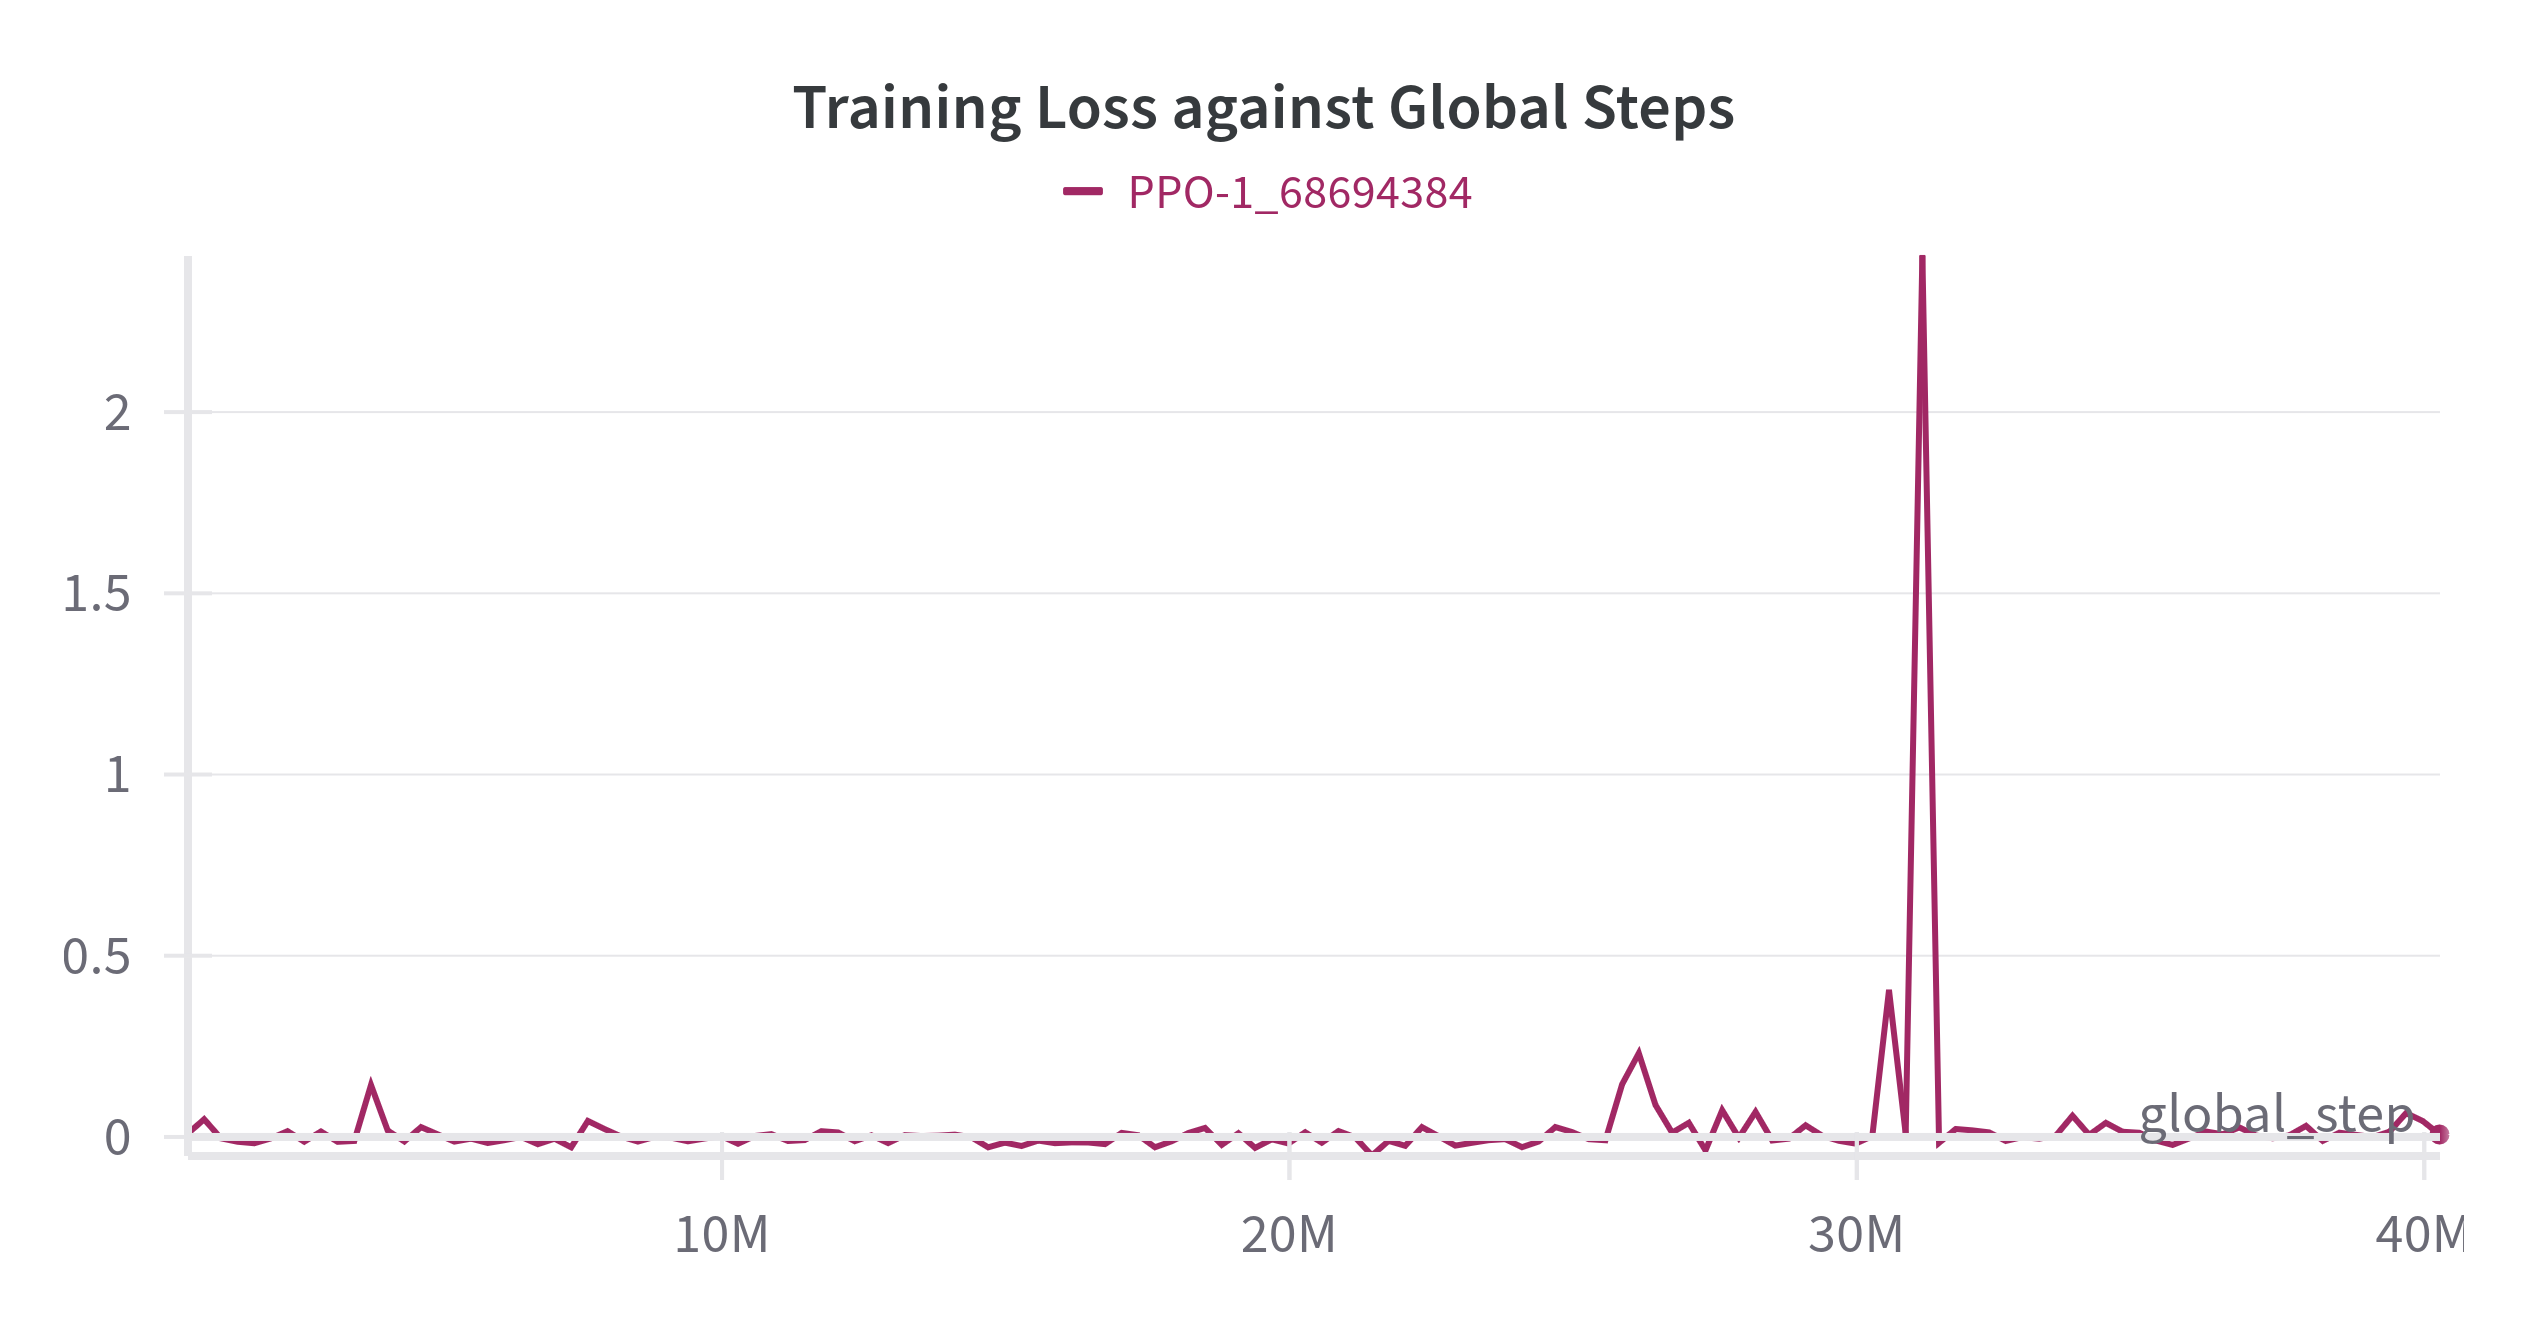
\includegraphics[width=0.49\textwidth]{figures/PPO/PPO1_Training_Loss.png}} 
    \subfigure[PPO-2]{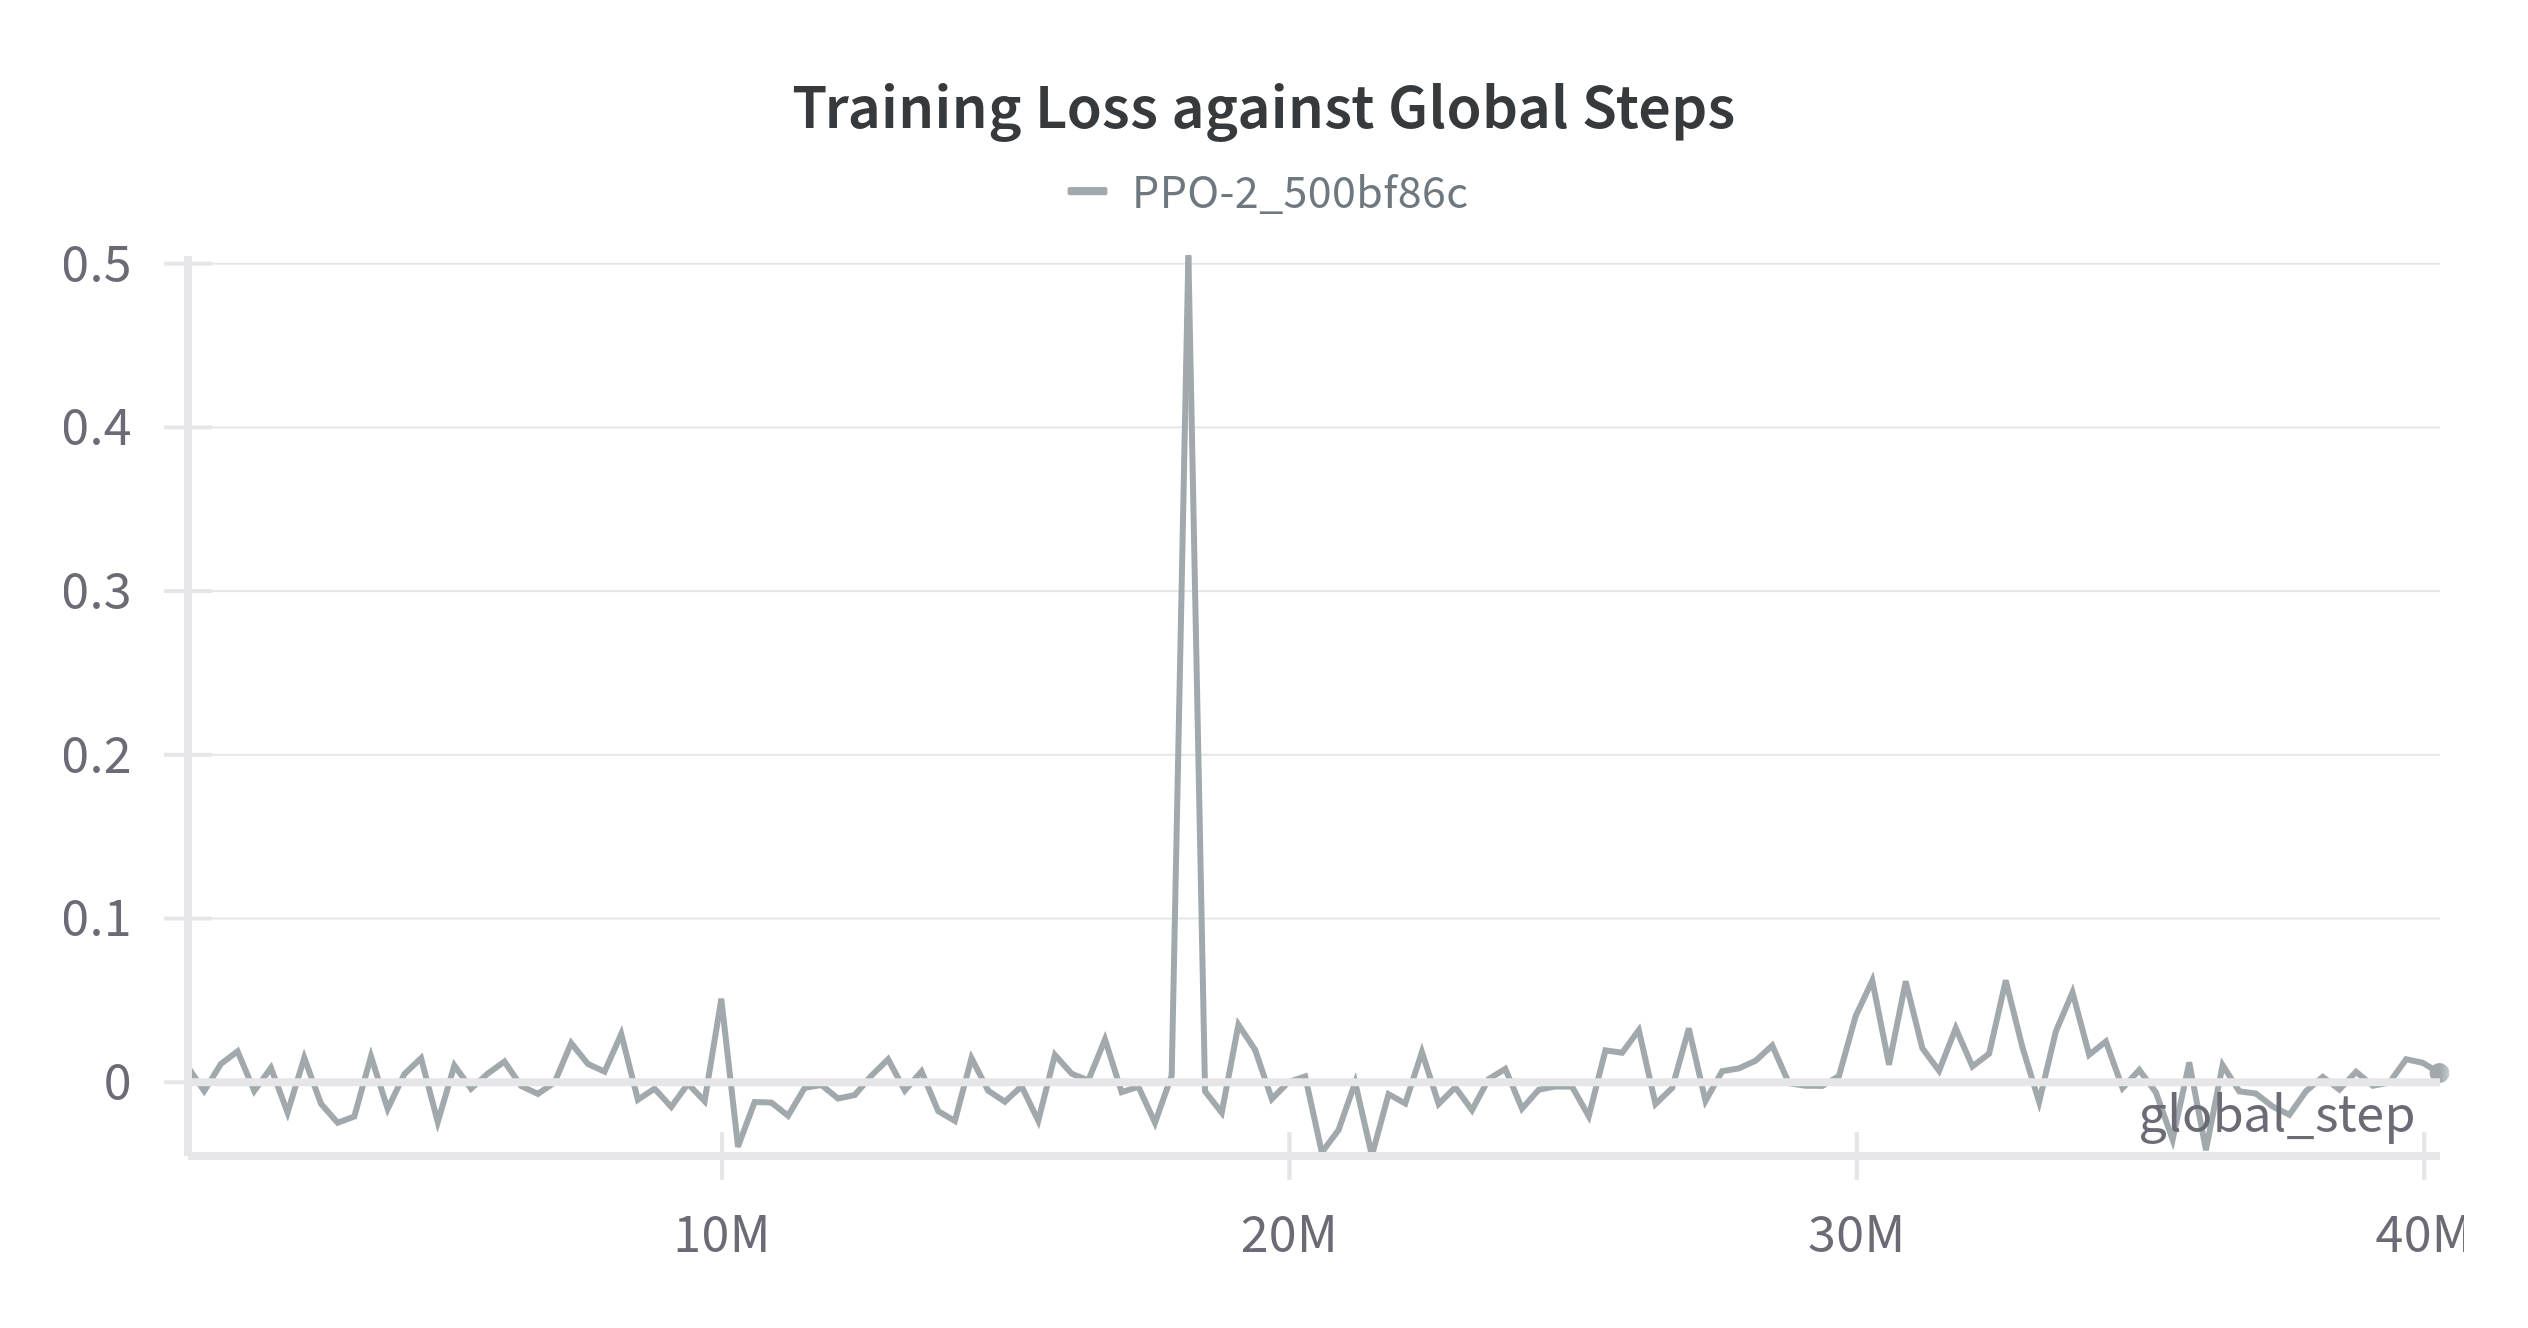
\includegraphics[width=0.49\textwidth]{figures/PPO/PPO2_Training_Loss.png}} 
    \subfigure[PPO-3]{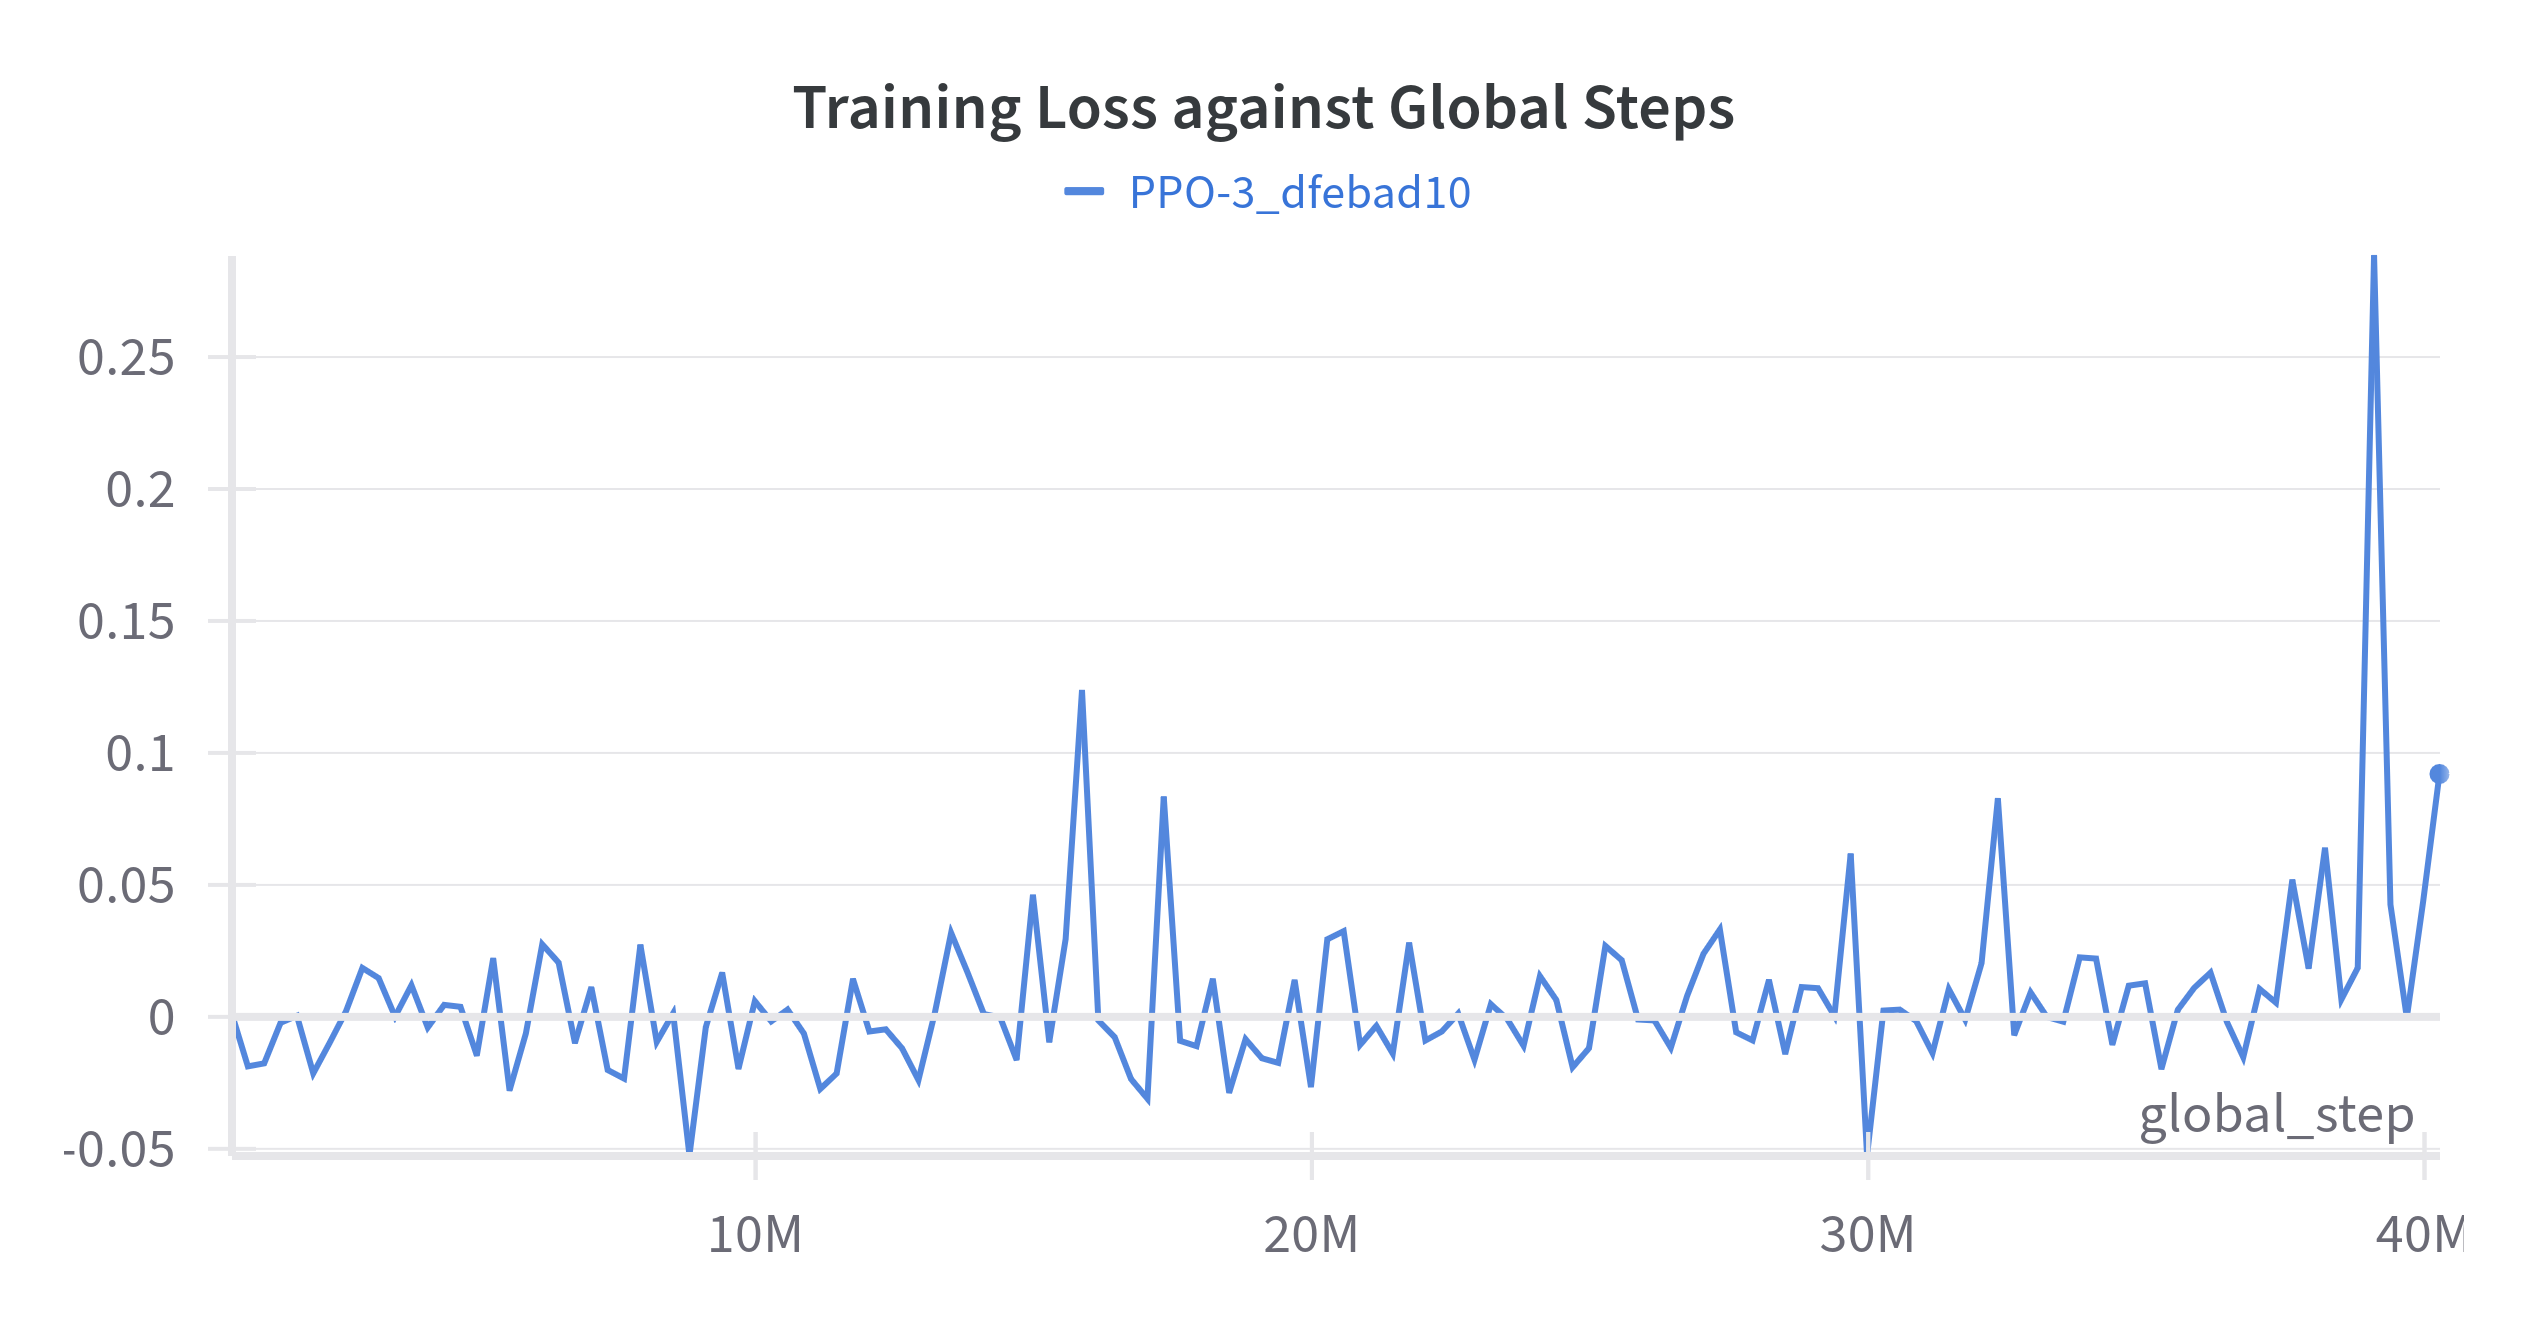
\includegraphics[width=0.49\textwidth]{figures/PPO/PPO3_Training_Loss.png}}
    \subfigure[PPO-4]{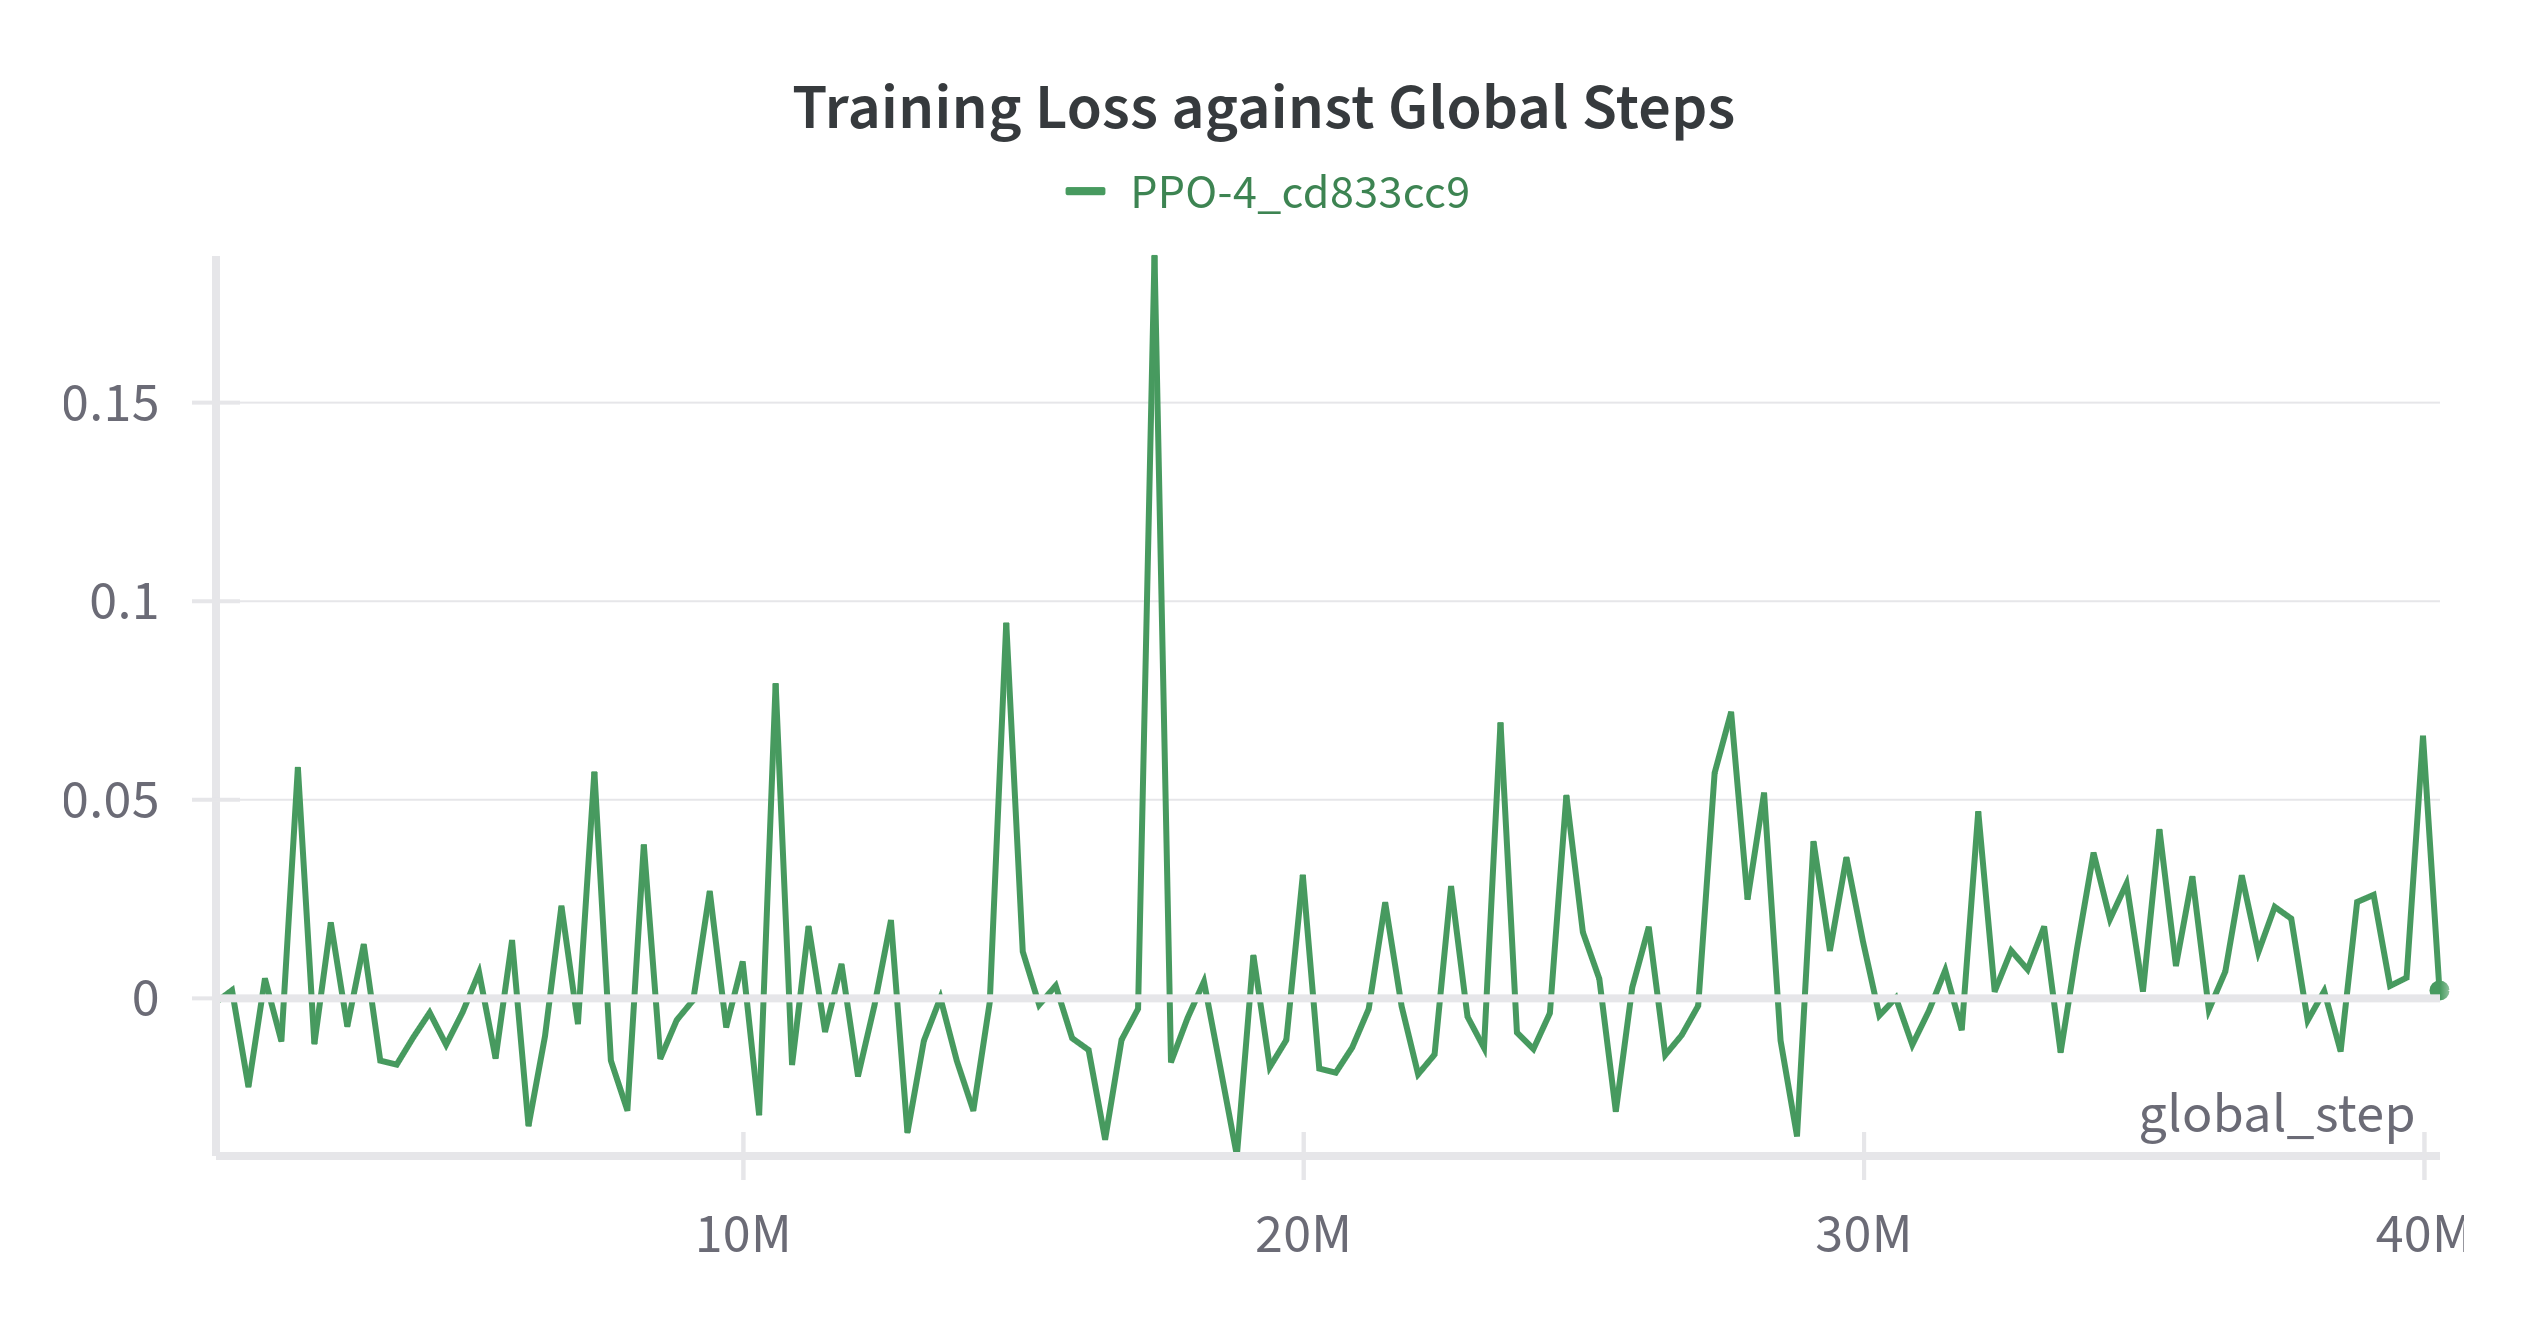
\includegraphics[width=0.49\textwidth]{figures/PPO/PPO4_Training_Loss.png}}
    \caption{Trianing Loss of all PPO Agents}
    \label{fig:PPO_training_loss}
\end{figure}

Figure \ref{fig:PPO_training_loss} shows the training loss of each agent and shows that all 4 agents had consistently low loss values throughout the training. All agents had a singular large spike in loss value but were able to recover from it. However, PPO-1's spike was of a value of 2.5 compared to the other agents, which had spikes of 0.15 to 0.5. This suggests that PPO-1 had a more inconsistent training process compared to the other agents. 

\subsubsection*{Badge Count}
\begin{figure}[H]
    \centering
    \subfigure[PPO-1]{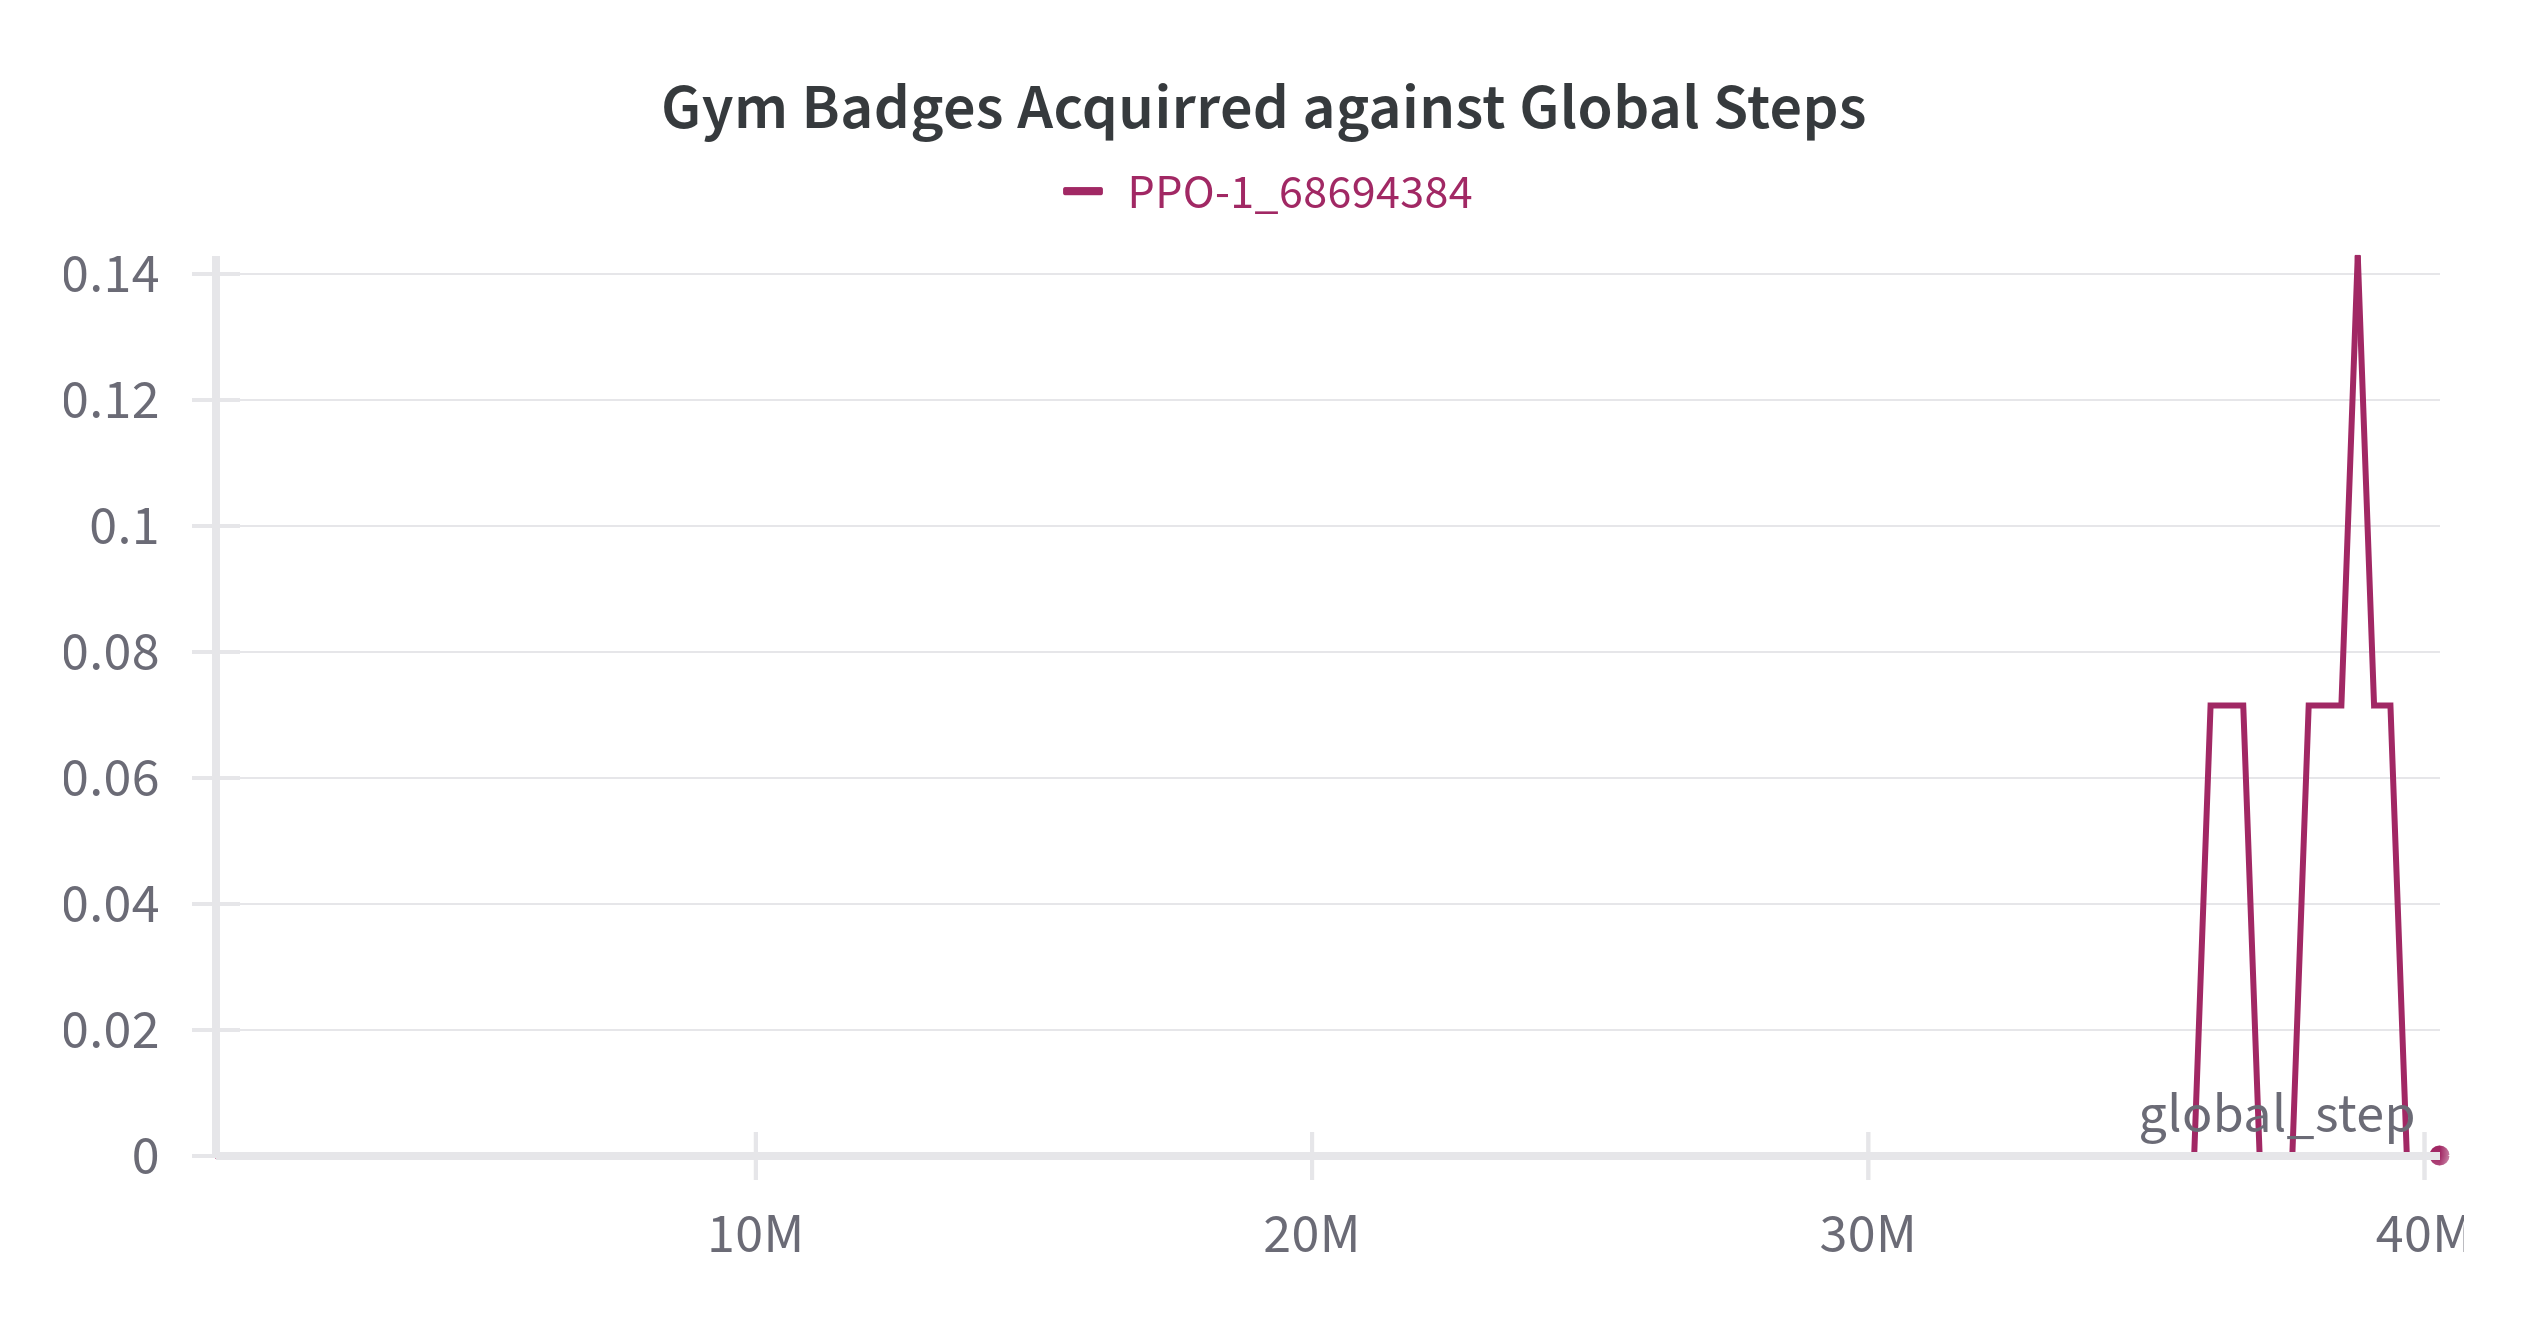
\includegraphics[width=0.49\textwidth]{figures/PPO/PPO1_Badge_Count.png}} 
    \subfigure[PPO-2]{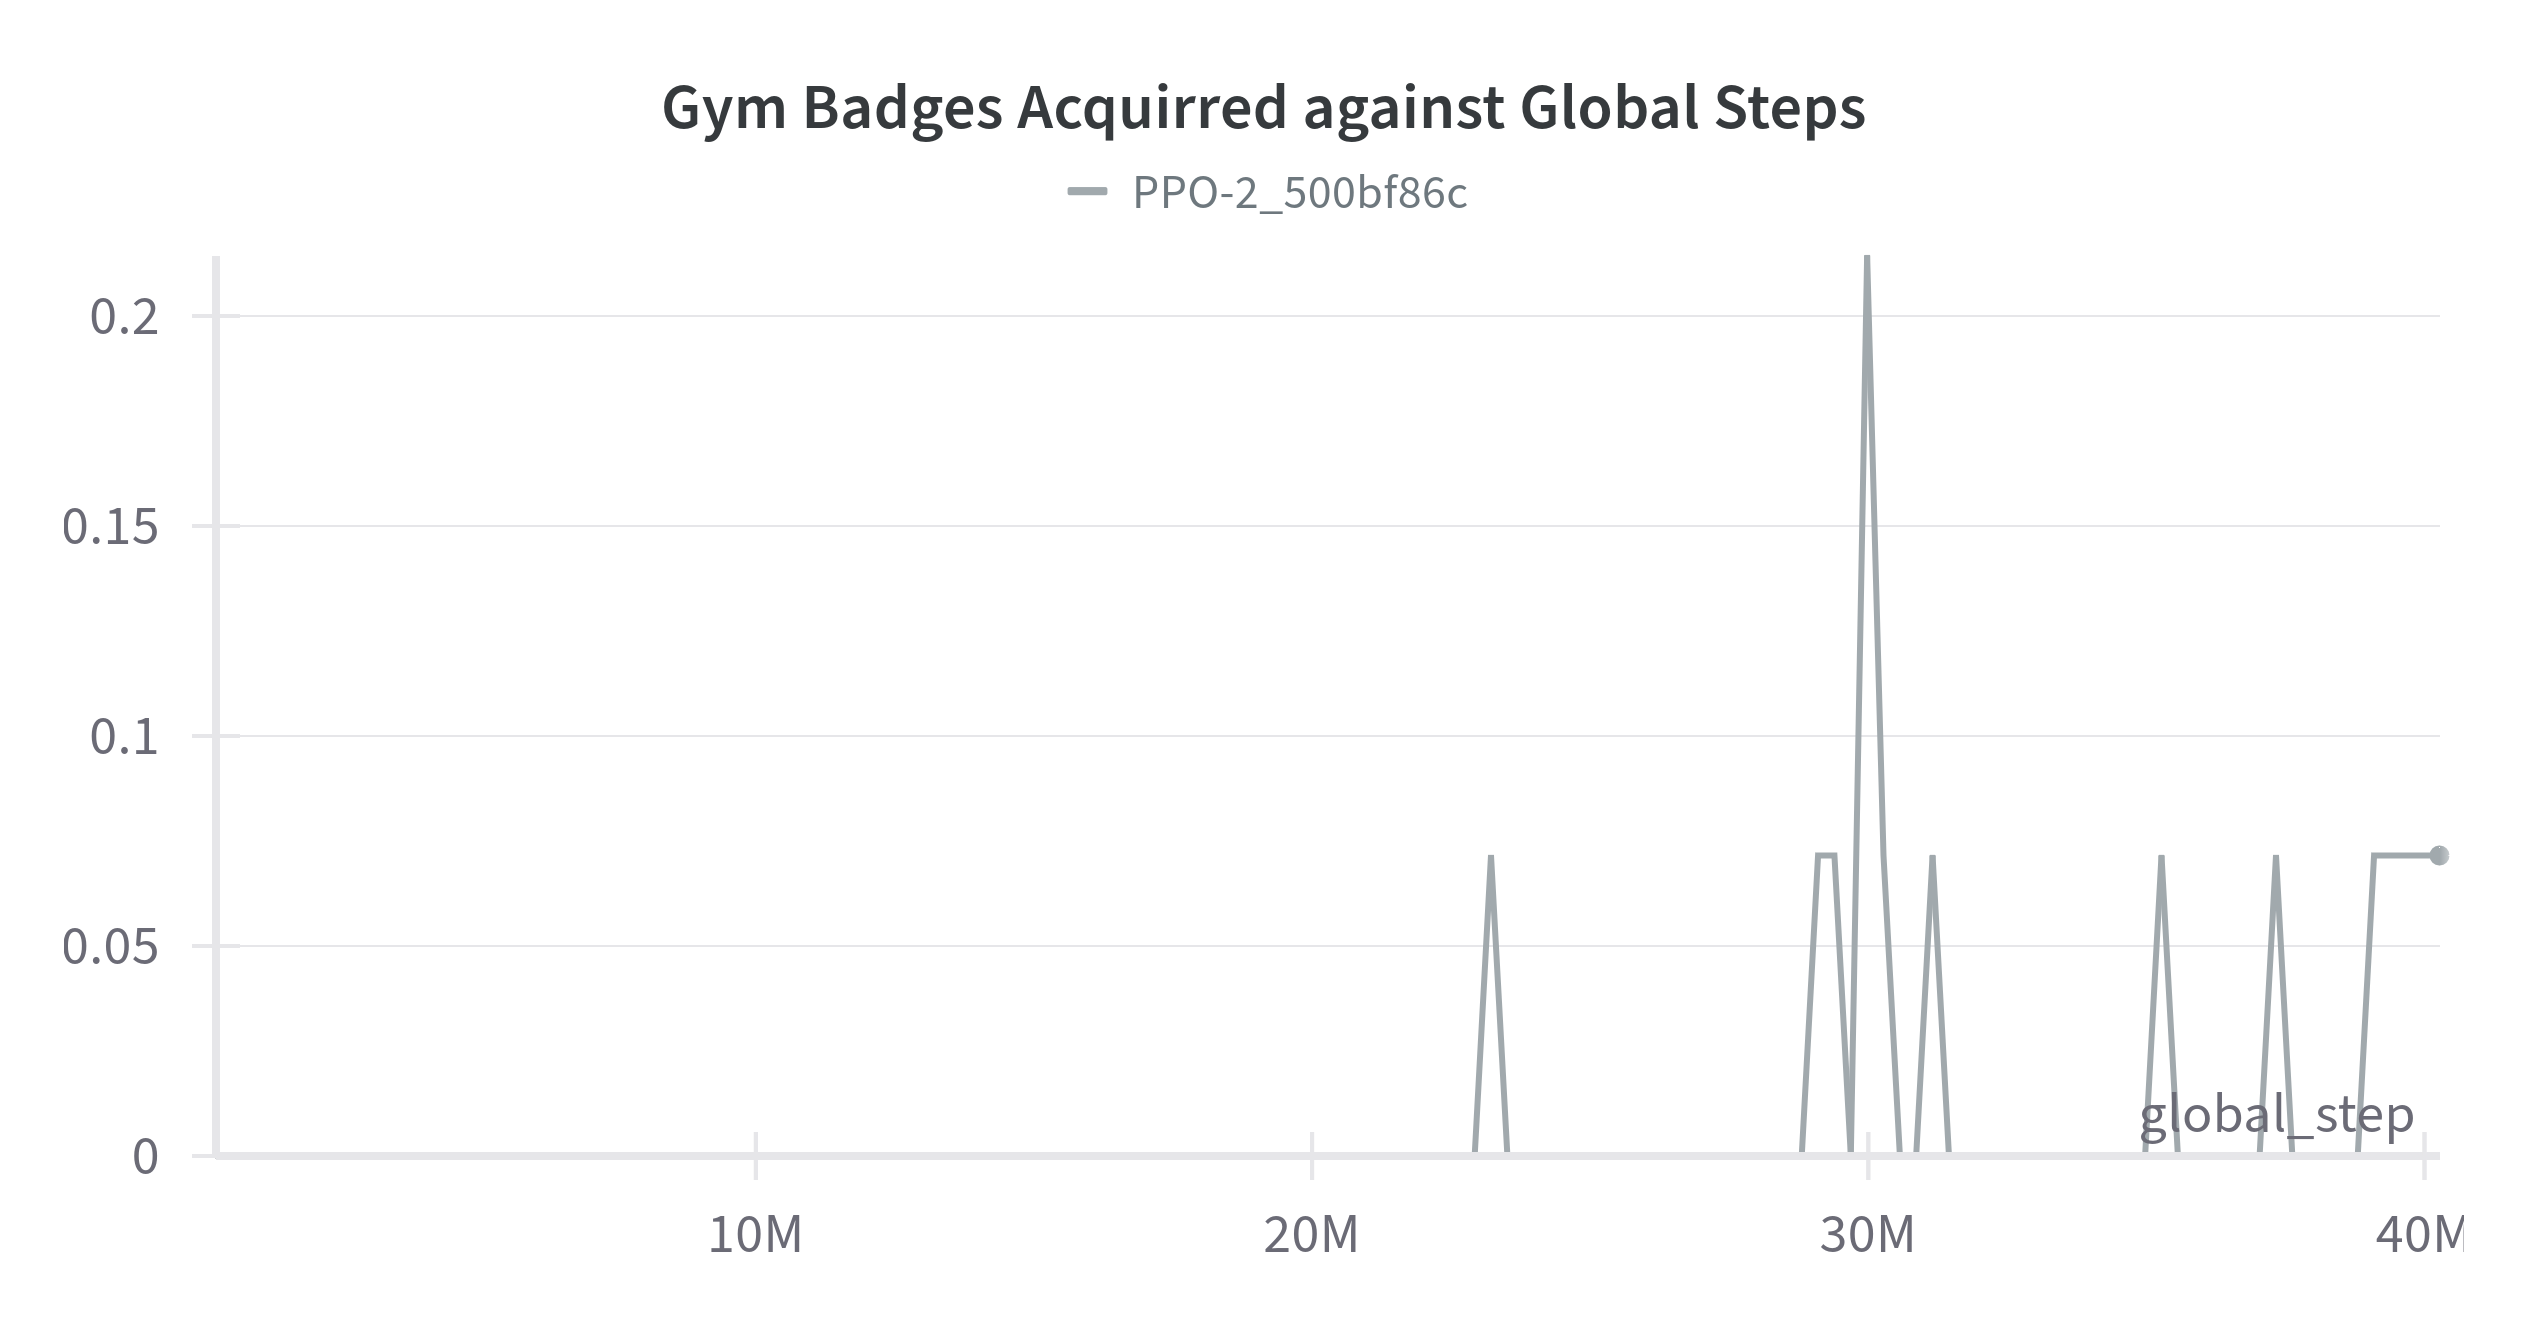
\includegraphics[width=0.49\textwidth]{figures/PPO/PPO2_Badge_Count.png}} 
    \subfigure[PPO-3]{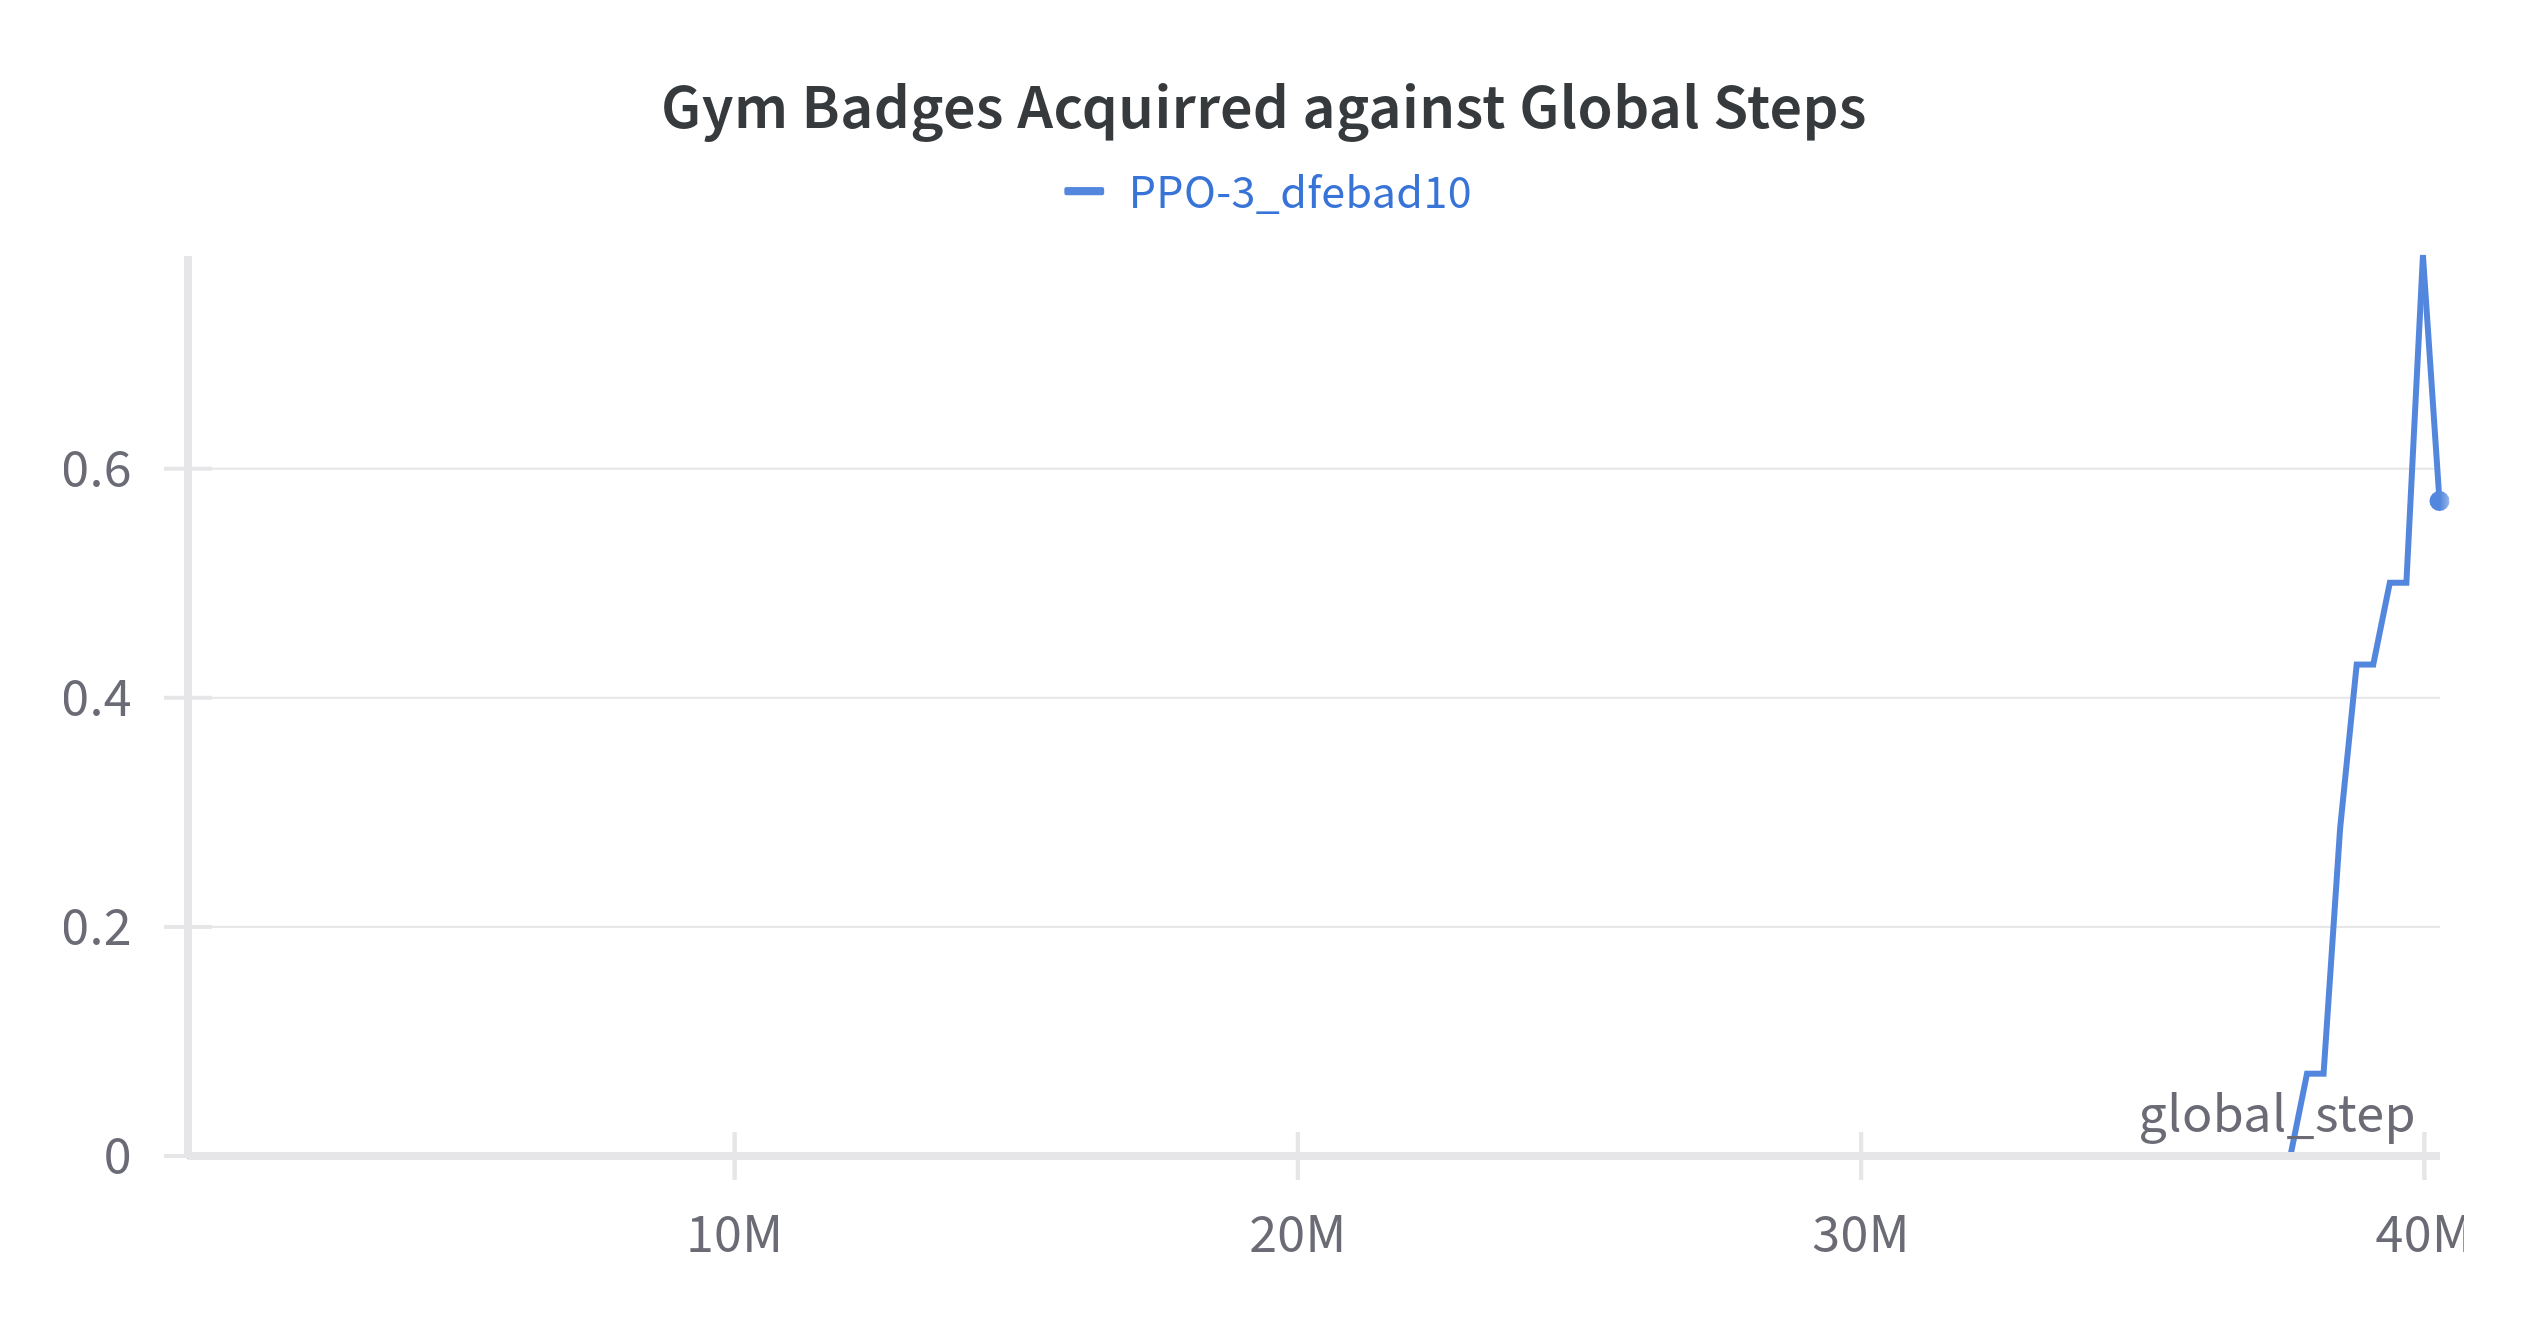
\includegraphics[width=0.49\textwidth]{figures/PPO/PPO3_Badge_Count.png}}
    \subfigure[PPO-4]{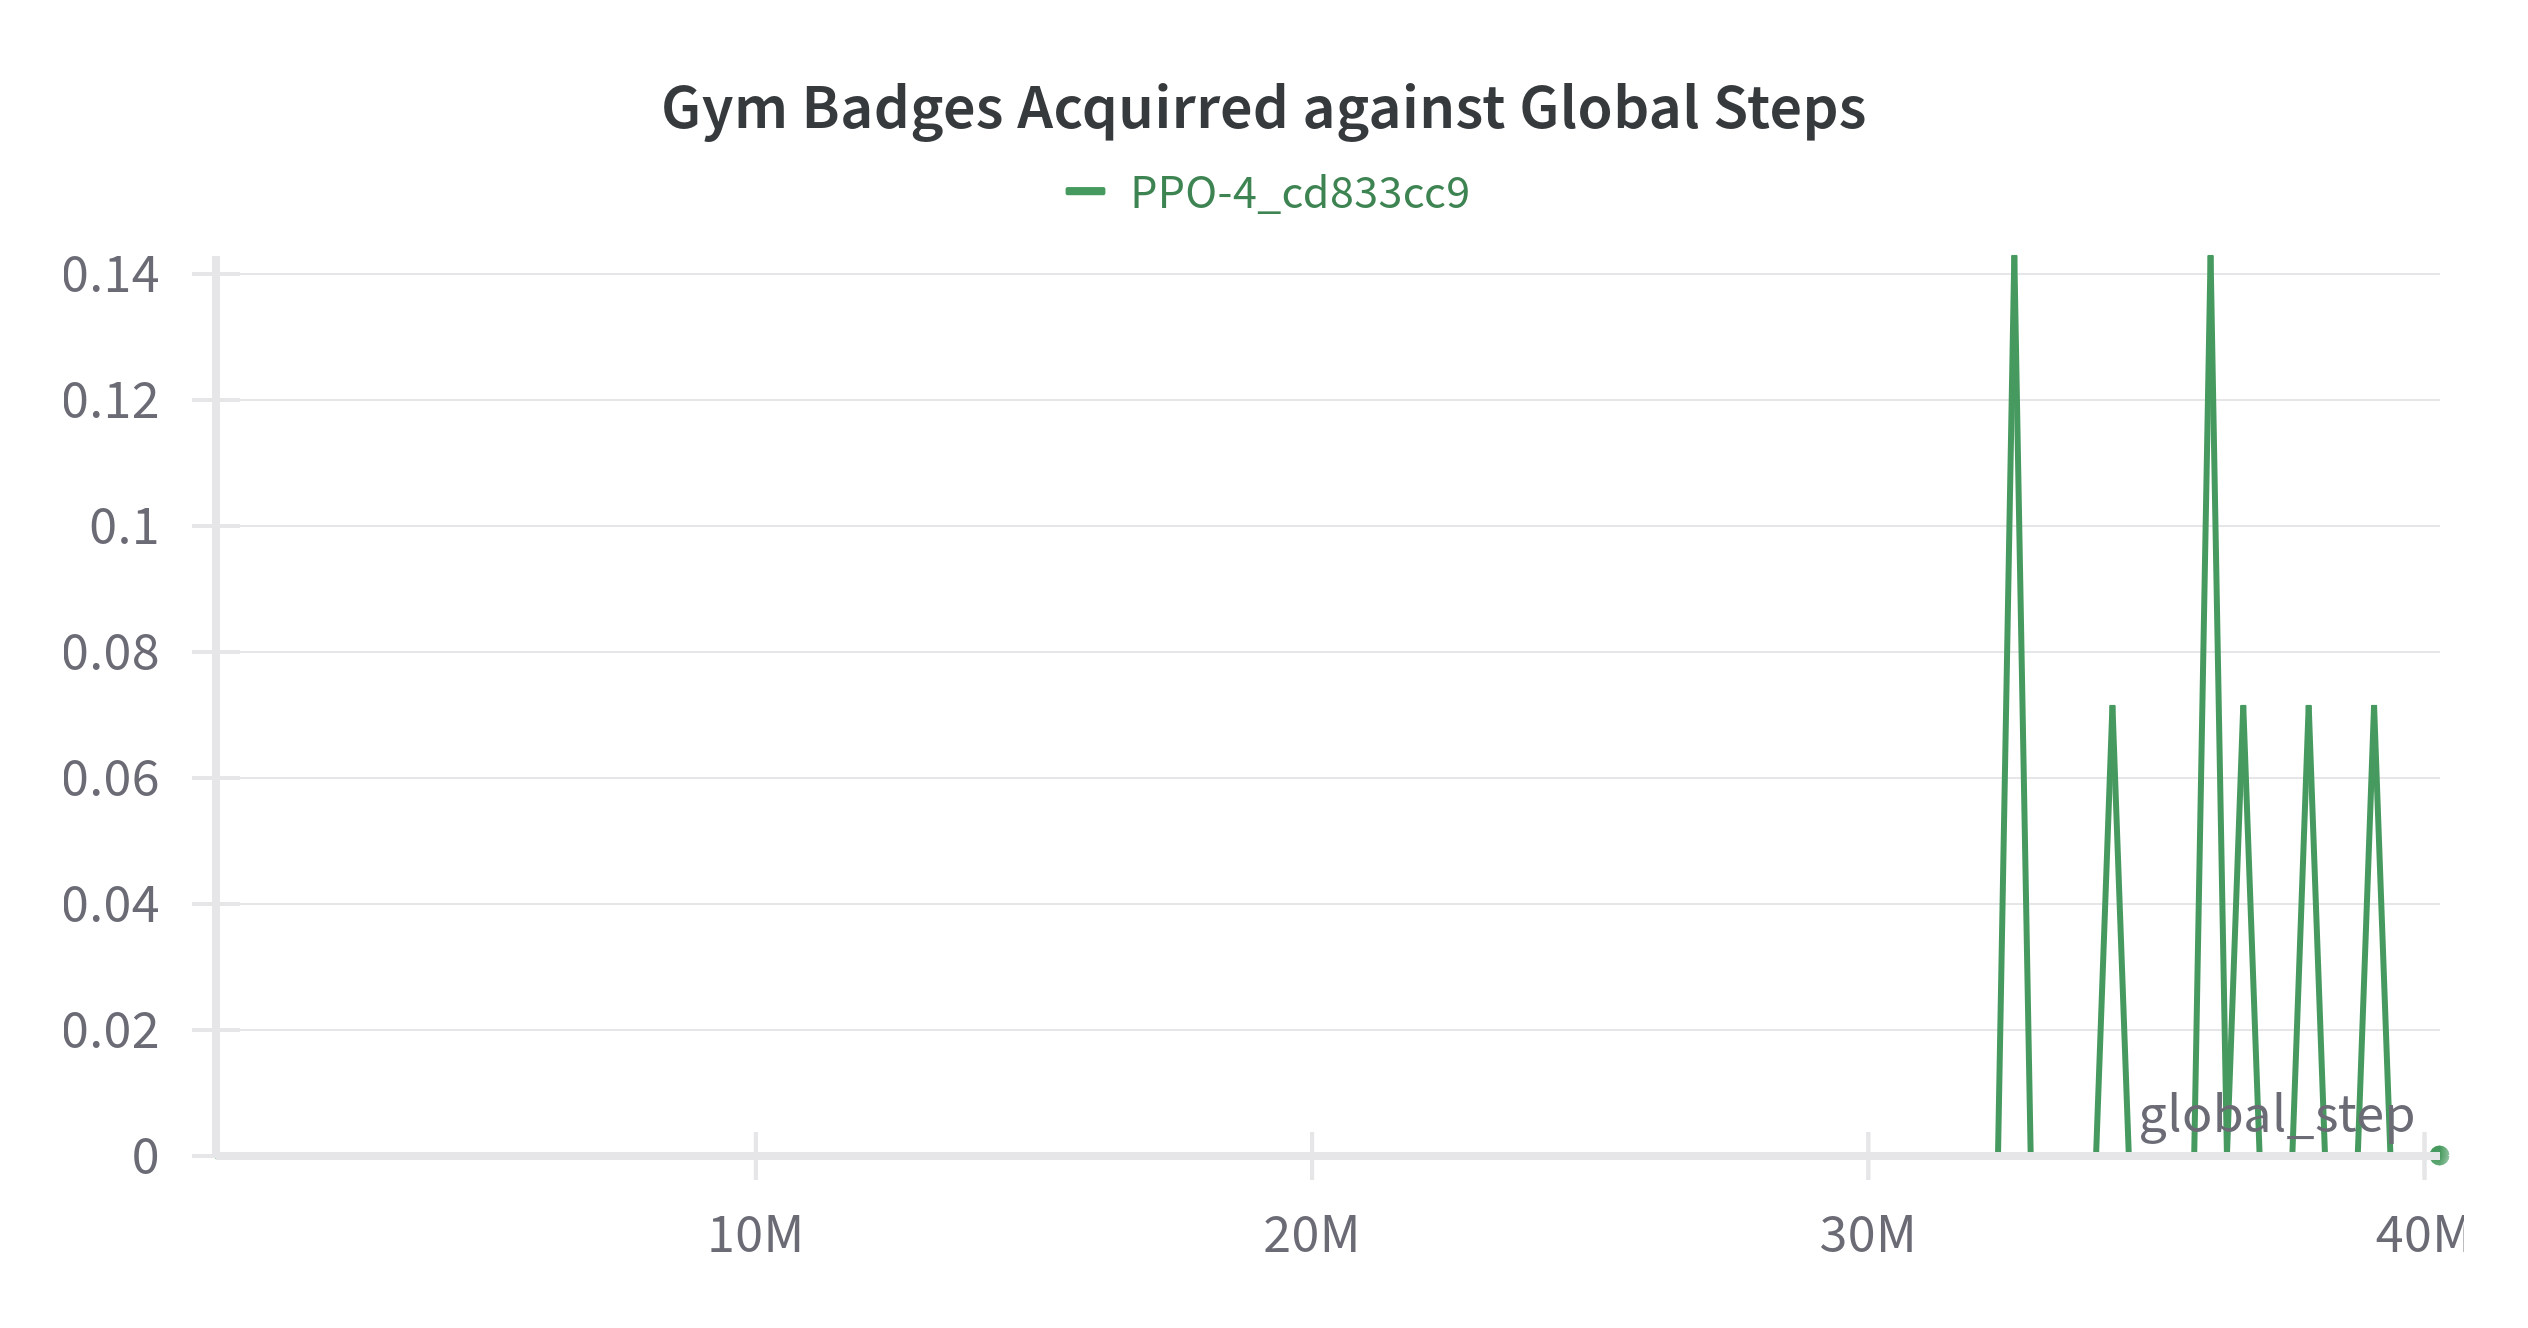
\includegraphics[width=0.49\textwidth]{figures/PPO/PPO4_Badge_Count.png}}
    \caption{Badge Count of all PPO Agents}
    \label{fig:PPO_badge_count}
\end{figure}

Figure \ref{fig:PPO_badge_count} shows the badge count of each agent and shows that all 4 agents were able to collect the first gym badge. This is already considerably better results than DQN and QRDQN and suggests that the agents were able to explore the environment effectively to reach the first gym badge. This is further confirmed by the total reward of each agent, as the difference in total reward between the start and end of training was significant. 

Figure \ref{fig:PPO_badge_count} (a) shows that the agent PPO-1 was able to collect its first badge after 36 million timesteps. Despite PPO-1 being able to collect a badge, the agent was the second slowest agent to collect the first gym badge. Moreover, the agent was also not the most consistent agent to collect the first gym badge.

Figure \ref{fig:PPO_badge_count} (b) shows that the agent PPO-2 was able to collect its first gym badge after 23 million timesteps. PPO-2 was the first agent to collect the first gym badge, which suggests that the agent was able to explore the environment the most effectively out of the 4 agents. However, it was not able to consistently collect the first gym badge.

Figure \ref{fig:PPO_badge_count} (c) shows that the agent PPO-3 was able to collect its first gym badge after 37 million timesteps. PPO-3 was the slowest agent to collect the first gym badge, but was the most consistent agent to collect the first gym badge. At 39 million timesteps, 80\% of the instances of PPO-3 were able to collect the first gym badge.

Figure \ref{fig:PPO_badge_count} (d) shows that the agent PPO-4 was able to collect its first gym badge after 32 million timesteps. PPO-4 was the second fastest agent to collect the first gym badge. In addition, after collecting its first gym badge, the subsequent episodes were able to collect the first gym badge consistently. However, only 10\% of the instances of PPO-4 were able to occasionally collect the first gym badge.

\subsubsection*{PPO Conclusion} 

To come to a conclusion as to which PPO agent is the best performing agent, figure \ref{fig:PPO_badge_count} showing the badge count of each agent will be used to determine which agent was able to complete the objective of this research the best by collecting the first gym badge the most consistently. The graph shows that all 4 agents were able to explore the environment enough to collect the first badge, however, PPO-2 was the agent to collect the first badge the earliest during training at episode 76. This is interesting as around the same episode, PPO-4 had a higher total\_reward than PPO-2. This suggests that the environment was explored differently by each agent and that the environment's reward function was not able to effectively guide the agent to reach the goal of collecting the first gym badge. Another interesting piece of information the graph confirms, is that agent 1 is the worst performing agent, as it was the second slowest agent to have one of the 10 instances collect the first gym, but also the agent with the least amount of consistency of instance of agents collecting the first gym badge. 

The most striking piece of information from the graph shows that PPO-3 was the last to collect the first gym badge, but was the agent with the most consistent amount of instances to collect the first gym badge. With a peak of 80\% of the instances collecting the first gym badge by the end of training. This confirms that PPO-3 is the best performing agent out of the 4 PPO agents.

\subsection{Algorithm Comparison}

The best performing agent from each algorithm will be compared to each other to determine which agent was able to balance out battling and navigation the best. The best performing agent from each algorithm was DQN agent 3, QR-DQN agent 1 and PPO agent 3. The performance of each agent will be compared through the use of comparing the total reward, loss, and badge count of each agent to determine their potential to complete the entire environment and how well they are able to achieve the objectives of this research within the training time frame of 40 million steps. 

One issue that arose while comparing the agents was that the agents were trained for different number of total episodes. Despite the total amount of timesteps being consistent betwewen all trained agents, the total amount of episodes was different because each algorithm had inconsistent number of instances of the environment being trained at the same time. This is because each algorithm took different amounts of RAM to train. Therefore, the graphs below will show the total timesteps taken on the x-axis instead of the total episodes. Next time, the number of environment instances and episodes will be kept consistent for further fairer testing. 

\begin{figure}[H]
    \centering
    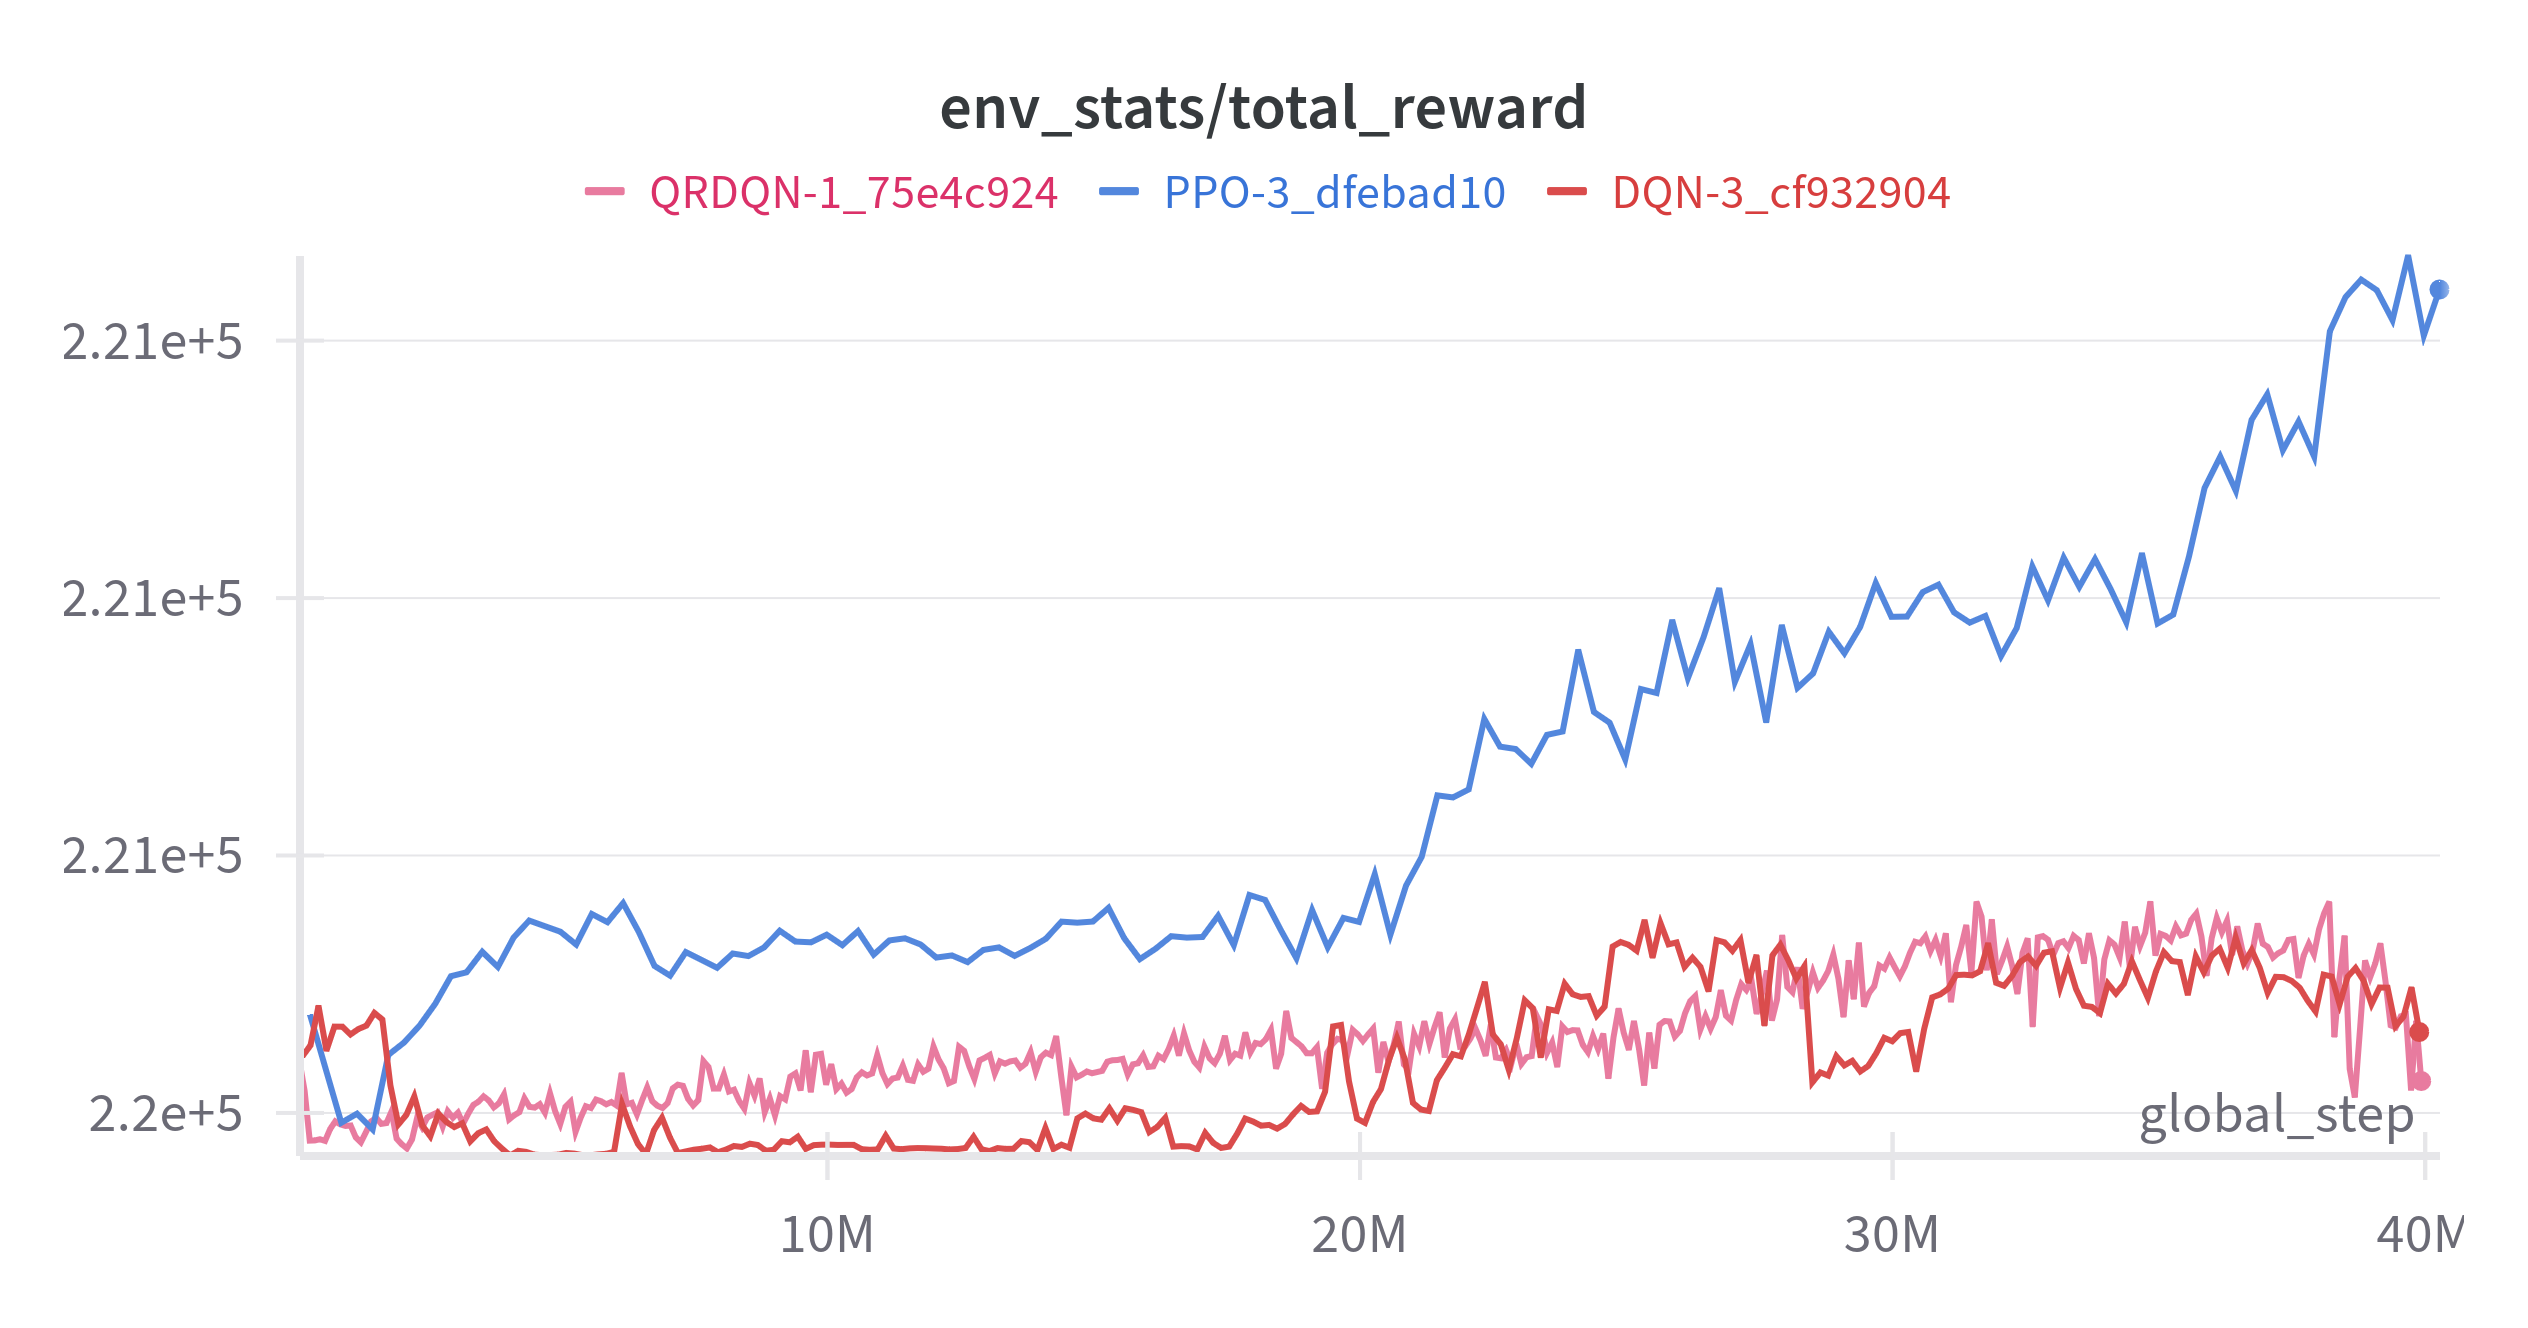
\includegraphics[width=0.8\textwidth]{figures/all_step_total_reward.png}
    \caption{}
    \label{fig:agent_eval_all_reward}
\end{figure}

Figure \ref{fig:agent_eval_all_reward} shows the total\_reward against total timesteps shows very evidently that PPO out performed DQN and QRDQN since the start. PPO was able to reach a higher amount of total reward within the first million timesteps compared to DQN and QRDQN. However, all 3 agents had similar rates of growth between 1 million and 20 million timesteps, which is suggested by the slopes of the agents being very similar. PPO showed a large increase in performance at around 20 million timesteps, which suggests that the agent was able to surpass a region of the environment which allowed for more reward to be gained. DQN and QRDQN comparitively did not show any signs of improvement in performance, which suggests that the agents were not able to reach the same region of the environment that PPO was able to reach. This is evident on figure \ref{fig:agent_eval_all_badge} below, showing the number of badges collected by each agent.

\begin{figure}[H]
    \centering
    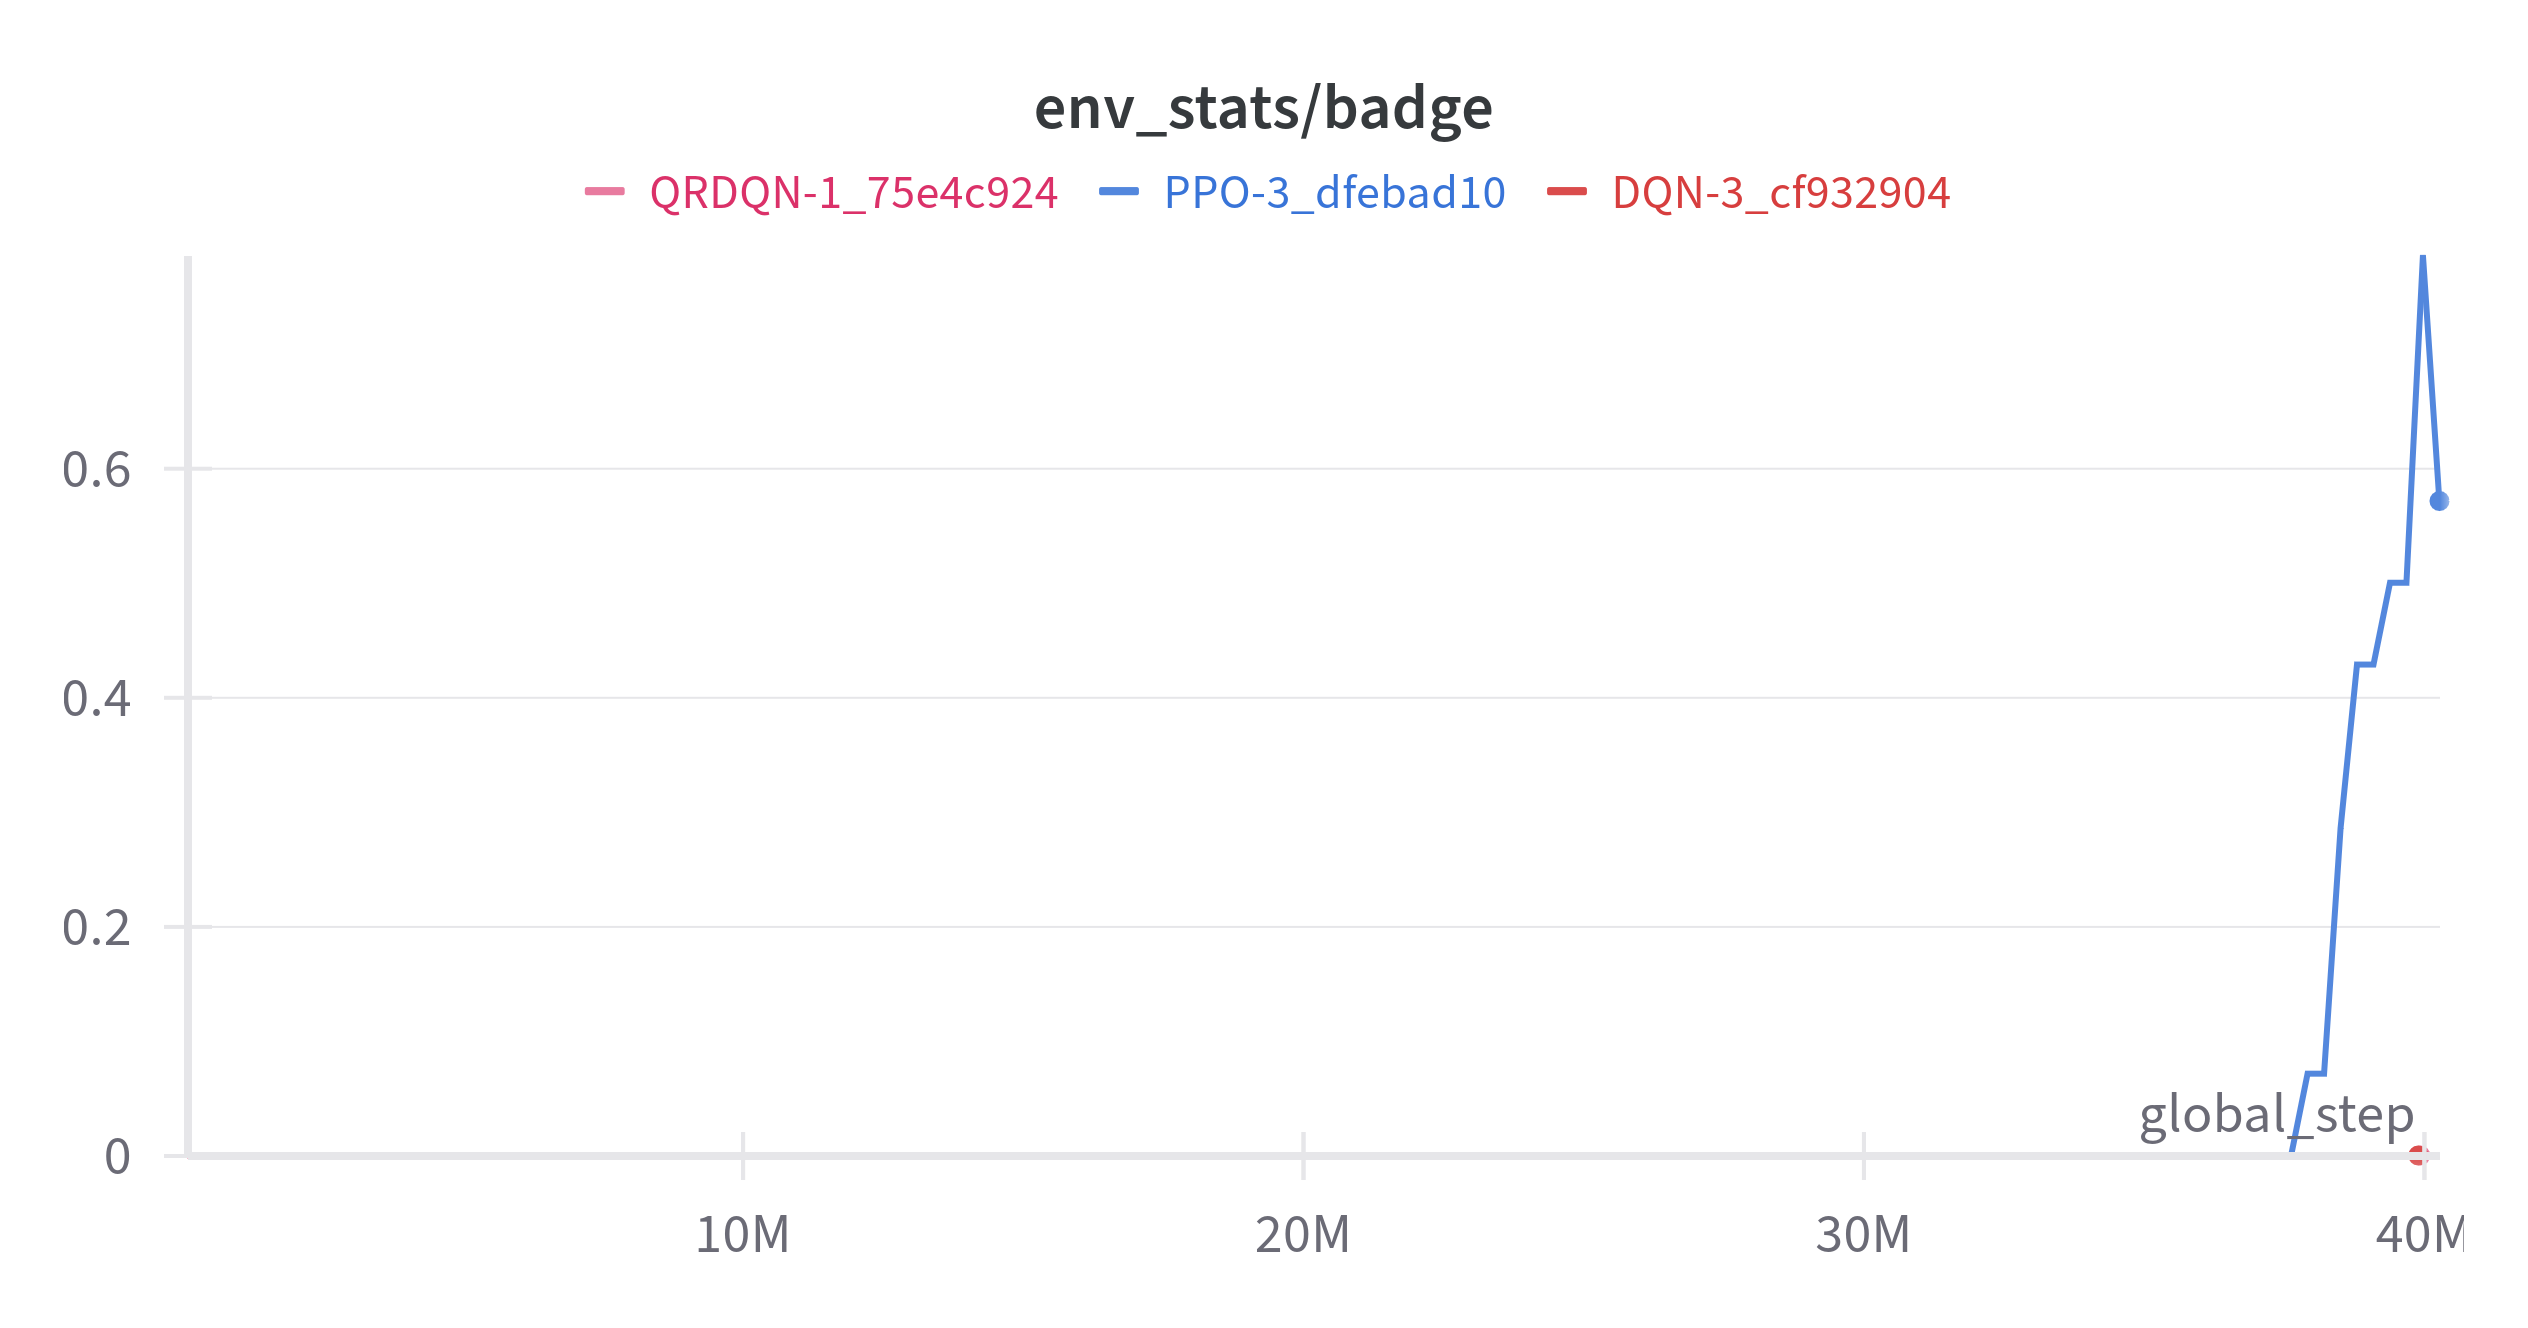
\includegraphics[width=0.8\textwidth]{figures/all_step_badge.png}
    \caption{}
    \label{fig:agent_eval_all_badge}
\end{figure}

This next graph shows the badge count of each agent against total timesteps. The graph shows that PPO was able to collect the first gym badge, where as DQN and QRDQN was never able to find the first gym badge. This suggests that PPO was able to explore the environment and overcome the challenges that DQN and QRDQN were not able to overcome, which is why PPO was the only agent able to collect the first gym badge. 

\begin{figure}[H]
    \centering
    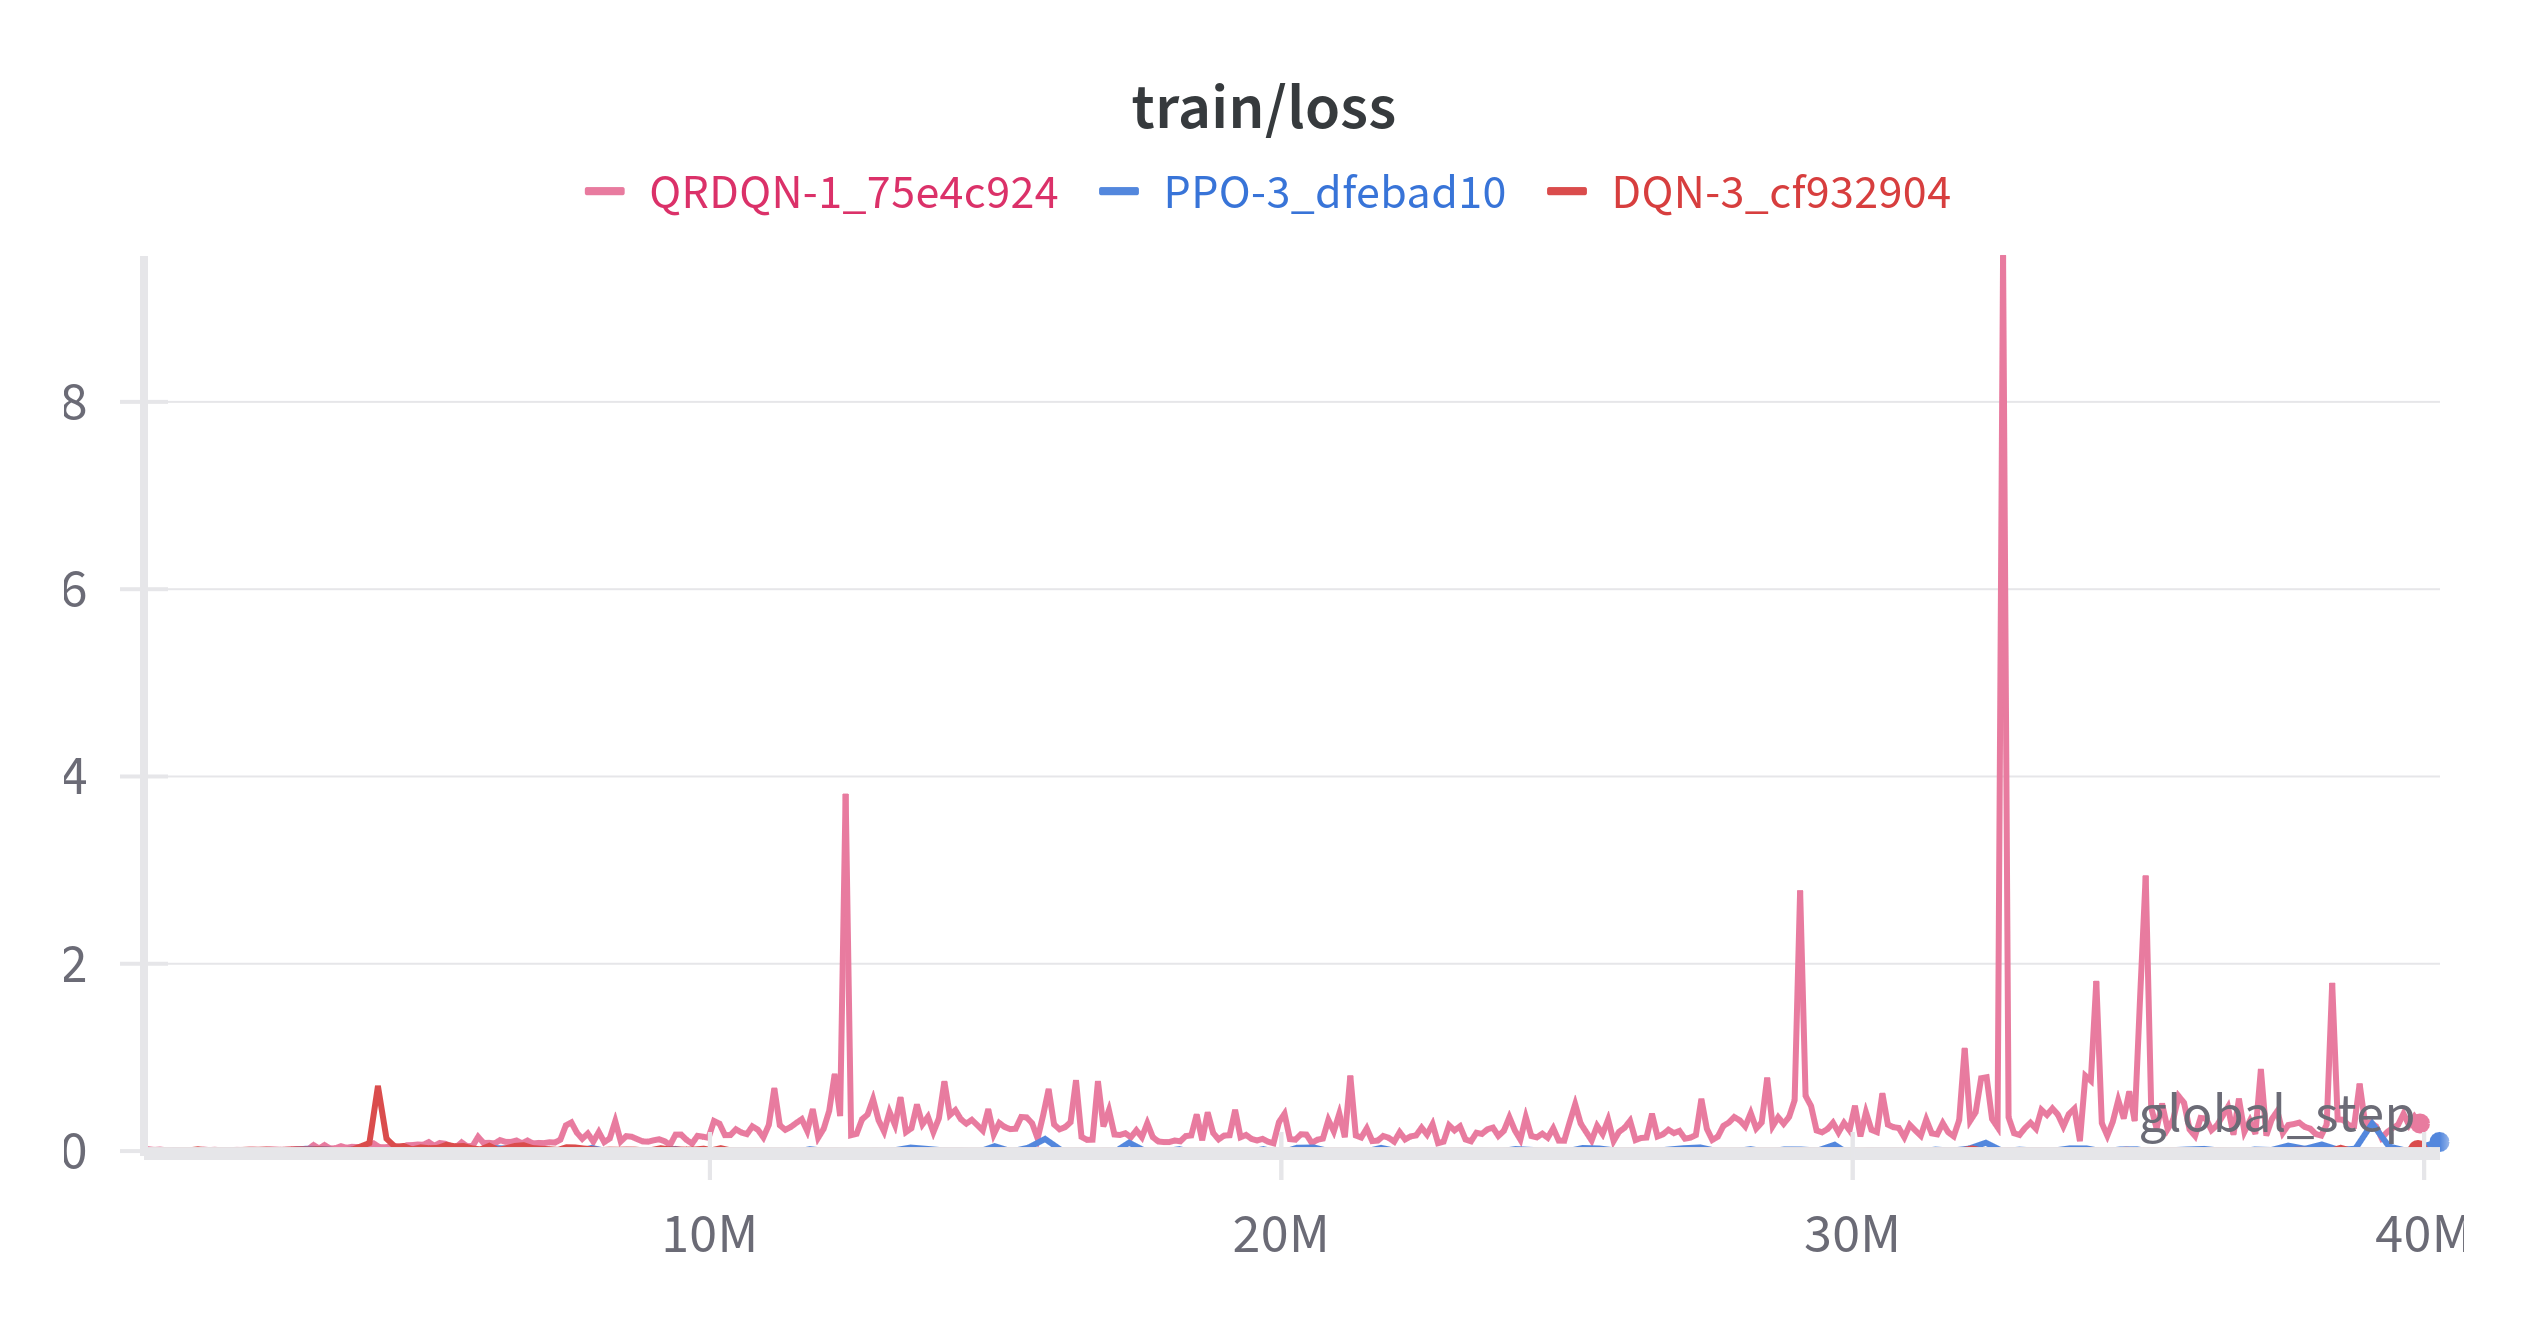
\includegraphics[width=0.8\textwidth]{figures/all_step_loss.png}
    \caption{}
    \label{fig:agent_eval_all_loss}
\end{figure}

Figure \ref{fig:agent_eval_all_loss} shows the loss of each agent against total timesteps. The graph very evidently highlights the turbulent nature of QRDQN training, as the agent had countless spikes of differing sizes. Where as DQN and PPO had very consistent low loss values throughout the training. This suggests that QRDQN had a very inconsistent training process and was not able to effectively learn what to expect within the environment compared to the actual outcome of the environment. It can be argued that the inconsistent training process is due to the low amount of reward achieved by QRDQN, which suggests that it was consistently exploring. However, the DQN agent had very similar levels of total reward to QRDQN and had a very consistent and low loss value while training. 

\subsection{Algorithm Comparison Conclusion}

In conclusion, it is evident that the PPO agent was the best performing agent out of the 3 agents. This is evident by the agents higher total reward, the only algorithm able to collect the first gym badge and the consistent low loss value throughout training. This suggests that value-based policies such as DQN and QRDQN are not as effective as policy-based policies such as PPO when training agents to explore and exploit the environment. However, it is difficult to find further research that agree with this conclusion, as there is a lack of benchmarks for multi-objective RL in the field. Moreover, there is a lack of popular well-known multi-objective RL environments that can be used to benchmark different algorithms unlike single objective RL. Despite the lack of benchmarks and research, Jett Wang's work using PPO to train agents to compete at high levels of pokemon battling suggests that PPO is a good algorithm to use for complex environments \cite{wang2020playing}. This is backed up by fact that Jett Wang's work was able to achieve far higher results than other works that focus on creating agents to do pokemon battling, while training the agent in a far more complicated environment. 

The other work to compare my findings to would be Flaherty, Jimenez and Abbasi's work in which they did train agents to complete pokemon red. However, their work compared DQN and A2C, where they found that A2C outperformed DQN due to A2C's greater timestep efficiency \cite{flaherty2021playing}. This would make for a great comparison between PPO and A2C because A2C uses both value and policy-based methods to train agents. This was one of the reasons why I initally chose to compare A2C as well to determine if I could reproduce similar results and if PPO was even more efficient than A2C. However, due to the lack of time and resources, I was not able to get A2C to work within the environment. 

It is possible that the stochastic nature and massive search space of this environment made it difficult for value-based policies to learn the environment effectively. As it was infeasible to explore each and every possible state within the environment. On the other hand, the reward function was fine-tuned to the PPO agent, which could have been the reason for the PPO agent outperforming the other agents. The complexity of the environment and the stochastic nature of the environment made it very difficult to determine an effective reward function without training agents to estimate the effectiveness of the reward function. 

Despite the total reward performance of DQN and QRDQN being similar, the loss value of the DQN agent were better than QRDQN because of its stable performance throughout all 40 million timesteps. This suggests that DQN was able to learn the environment more effectively than QRDQN because of its ability to make consistent reward expectation throughout training.
